%%
%% Suspensions chapter
%%
%% Author:
%% Version:
%%
%\documentclass[color,cite,epsfig,12pt]{article}
%\usepackage{graphicx}

%\begin{document}
%%\bibliographystyle{unsrt} 


%\documentclass[color,cite,epsfig,12pt]{article}
%\usepackage{graphicx}

%\begin{document}


\FloatBarrier
\subsection{Description}
%
% put here the description of the content of the section
%
%\emph{
%Responsible:  WP2 coordinator, F.\ Ricci\\
%}

The suspension system of a gravitational wave detector is conceived to isolate the test
masses from ground seismic vibrations and local disturbances so that they are considered 
nearly in a free fall state in the frequency bandwidth of interest. 
A typical suspension chain is obtained cascading a set of passive mechanical filters
providing a suited attenuation from seismic and acoustic noise above a certain cut-off
frequency. Below this frequency value an active feed-back control strategy is developed 
by using sensors and actuators disseminated along the suspension chain and keeping the 
interferometer at its working point.
  
The upper part of the suspension chain, called \emph{Superattenuator} (SA), is essentially a 
N-stage pendulum supported by a three-leg elastic structure, called Inverted Pendulum (IP). 
In an N-stage pendulum the horizontal displacement of the suspension point, at a frequency 
$f$ much higher than its normal modes $(f_1, f_2, ........, f_N)$, is transmitted to the 
last stage with an attenuation proportional to $f^{-2N}$.
In order to attenuate the vertical vibrations, each mass of the multi-stage pendulum is 
replaced by a cylindrical mechanical filter with a set of concentric cantilever blade 
springs with low stiffness. The blades support, through a long metallic wire, the next 
mechanical filter, forming a chain of low frequency oscillators also in the vertical direction. 
In Virgo the blades work in parallel with a magnetic anti-spring system, assembled 
on each filter and designed to reduce its vertical mode from about 1.5 Hz down to 0.5 Hz. 
Thanks to the anti-springs the vertical modes of the chain are all below 3 Hz. 
Starting from a few Hz, the mirror is thus well isolated from vertical seismic noise too. 
 
The last suspension stage (LSS), called {\it {optical  payload} } or simply 
{\it {payload}}, is the system designed to couple the test mass to the SA chain, 
to compensate the residual seismic noise and to steer the mirror through internal 
forces exerted from the last SA element. The main components of a Virgo-like LSS are: 
the Marionette, the Recoil Mass (RM) and the Mirror. The marionette is the first 
stage used to control the mirror position by means of coil-magnet actuators acting 
between the last stage upper part suspension and the marionette arms, while the recoil 
mass is used to protect and to steer the mirror. On its mechanical structure, indeed, 
the coils of the electro-magnetic actuators acting on the mirror back side are mounted.

\noindent
LSS plays also another important role: all the mechanical elements which are connected 
to the mirror are designed not to degrade the intrinsic mechanical losses of the 
mirror itself. This is necessary because of the well known relation between mechanical 
dissipations and thermal motion in macroscopic systems. The thermal noise contribution 
is reduced by developing sophisticated suspension systems with materials having low 
mechanical dissipation and low friction mechanical clamps. However, to achieve  
the goal sensitivity of the ET Project at low and intermediate frequency, 
a further reduction of thermal noise contribution is obtained by cooling the mirror 
and its last stage at cryogenic temperature\cite{ricci_moriond}. Cryogenic operation 
introduces additional difficulties, but the benefits in thermal noise reduction 
is also enhanced by the materials selection with improved properties at low 
temperatures. 

\noindent
A major challenge for cooling the mirror is to provide an efficient path for heat 
conduction while still maintaining good thermal noise and mechanical isolation performance. 
The cooling system needs to provide adequate heat extraction from the test masses, 
for both steady state operation and for cooling from room temperature in a reasonable 
time, without adding noise or short-circuiting the mechanical isolation. This constraint 
has an important impact on the design of a last stage of cryogenic suspension.

In the next sections we analyze in sequence all these aspects and we will try to summarize 
a perspective solution for each of them presenting also possible alternative approaches. 
Finally, an overview of the related technologies to be developed is presentsd in section 4.6.

%
\FloatBarrier
\FloatBarrier
\subsection{Executive summary}
%

We organized the design study of the ET suspension focusing the activity on four main arguments:
\begin{itemize}
\item {The upper part of the suspension, the \emph{superattenuator} (SA),  providing 
the needed seismic and acoustic isolation. This issue is discussed and the solution 
is presented in the Upper Stage section~\ref{sec:Upper_stages_mechanics}; }
\item{The last stage (payload), crucial for the defining the thermal noise 
performances and the mirror control are presented in paragraph~\ref{sec:last_stage};}
\item{The local control strategy and the related instrumentation, analyzed in 
sections~\ref{sec:local_control}, \ref{sec:em_actuator}, \ref{sec:electrostatic};}
\item{An overview of the main technologies to be developed for achieving the ET 
scientific goal (see sec.~\ref{sec:crystal-production}, \ref{sec:bonding}, 
\ref{sec:accelerometers}).} 
\end{itemize} 

We notice that to clarify some of the open problems, several R\&D programs have been 
carried out with limited resources. In particular, a bigger effort should be done 
in the domain of the material studies and of the low temperature  sensing devices.  
Nevertheless we succeed in preparing a reference solution and a set of alternative 
scenarios for driving the ET technical design. However the solution selection 
requires intensive experimental activity and the coordination efforts will be  
significantly effective only if continuous activity in the laboratories is sustained 
and coordinated in collaboration with the Japanese project LCGT.

The preliminary activity of the ET working group, devoted to the conceptual design 
of the suspensions, was centered on the definition of ET suspension requirement. 
In particular we collected and compared the mechanical and thermal properties of 
the materials at room and low temperature. 
Both silicon and sapphire potentially offer superior performance at cryogenic temperatures. 
In particular silicon samples can be obtained in large cylindrical blocks of mass higher 
than 100 kg. Its attractive thermal and thermo-mechanical properties makes it a strong 
candidate for the mirror and the suspension fibre in the future detector operating 
at cryogenic temperatures. 

\medskip

The low and high frequency interferometers ( ET-LF and ET-HF) proposed in the ET 
design study require different suspension systems. In the following we will show 
that the SA as it is operating within the Virgo interferometer is already compliant 
with the HF interferometer requirements. On the other hand for  ET-LF a dedicated 
effort is required. In fact, to extend the detection bandwidth of the Einstein 
Telescope in the low-frequency region starting from a couple of Hz, a better seismic 
attenuation in the ultra-low frequency range is needed. 
The \emph{Superattenuator} dynamics in the low frequency range, where the inner 
normal modes of the mechanical filter chain are confined, has been simulated by 
using the electro-magnetic equivalent circuit and a detailed simulation campaign 
devoted to this design study has been performed. On this base we concluded that 
we can fix to six the number of filters because a better attenuation performance 
in the high frequency range is not necessary anymore since the safety margin is 
large enough in Advanced Virgo and even larger in an underground environment. 
Then, a SA 17-m high with six magnetic anti-spring filters ("equal-spaced" 
configuration) tuned with a vertical cut-off frequency around 300\,mHz, represents 
the reference solution for  ET-LF interferometer. 

\medskip

As we anticipated above, the last stage of the suspension system is crucial in defining 
the suspension thermal noise performances. In particular for the  ET-LF case we deal 
with a system of coupled oscillators with masses at different temperature. For this reason, 
the thermal noise evaluation required to develop a specific model,where
the interacting masses are at different  temperature in steady state condition. 
The study of the thermal noise 
of this system has been carried on by using two different methods and the suspension 
thermal noise curves have been compared with the ET-D goal sensitivity curve driving 
the design of the last stage of the mirror suspension. 

Thus, the conceptual design of the payload for LF and  ET-HF has been completed. 
It includes for  ET-LF the analysis of the heat flow, the definition of the fibre 
material and geometry and the heat path from the mirror to the cold box via the 
marionette trough the suspension fibres and the dedicated heat sinks.

\medskip

The  ET-LF payload will be installed in the lower part of the vacuum tower hosting 
the 17-m long super-attenuator chain. The vacuum tower basement is a cryostat separated 
to the upper part by a roof crossed by the Ti-6Al-4V thin rod, which holds the 
whole payload. The cold box is set on top of a cryo 
compatible attenuator chain hosted in an ancillary cryostat. The box will keep the mirror at cryogenic temperature: 
it can be either a simple liquid helium container in the case of a cryoplant based 
on cryofluids or the cold head of a cryo refrigerator in the case of a cryocooler 
plant. Both solutions are discussed and compared in more details in the infrastructure 
section. The final choice will depend on the outcome of a dedicated  R\&D effort.

\medskip

A sophisticated control systems will be implemented in order to hierarchically 
control test mass positions to bring the interferometer to operation.
The actuation system is needed to align the interferometer mirrors 
and to automatically maintain the operation point. It is based on the signals 
derived from the circulating light  to apply internal forces exerted 
through the last stages of the suspension. 
The actuation based on a coil-magnet system for ET is reviewed in details and 
its limit associated to the $1/f$ potential noise is assessed; the alternative 
electrostatic approach is also discussed.

\noindent
For the  coarse mirror control optical conduits and bundle fibre served as position sensors have been tested  at low temperature  \cite{VFC}. They can be used together with short-arm optical levers and small 
interferometric systems for fine position control to achieve an alignment accuracy within 
10 nrad RMS. Hence low frequency cryogenic accelerometers have being developed 
for this purpose.

\medskip

Finally, it should be underlined that the complex study on the ET suspension system 
is not limited to a definition of a reference solution. Some crucial technologies 
to be developed in the domain of the slicon fibre and cryo-device construction have
been identified. These are issues of potential interest for industrial world too.


 
% \end{document}>>>>>>> .r616


\FloatBarrier
\subsection{Mechanics of the suspension upper stages }
\label{sec:Upper_stages_mechanics}
%\emph{
%Author(s): S.\ Braccini, F.\ Frasconi}
\FloatBarrier
\subsubsection{LF interferometer}

In this paragraph we discuss in details the problem of the attenuation of the seismic noise  and we present  a possible solution for both ET-LF and ET-Hf interferometers.  The focus is set on a Virgo {\emph {Superattenuator}} solution. In fact, it has been experimentally demonstrated \cite{Collaboration2010} that this solution provides already a seismic noise attenuation of  more than ten order of magnitude starting from a few Hertz.  Alternative approaches are cited in the Appendix, where the geometric anti-spring and the active filter developed in LIGO, GEO, TAMA  and at the NIKHEF laboratory are  described. The material compatibility of the \emph{Superattenuator} with a cryogenic environment is discussed also there.
In the following we will present in sequence

\begin{itemize}
\item  The ET attenuation requirements
\item The Virgo Superattenuator
\item Seismic isolation measurements with the Superattenuator (SA)
\item SA modifications for Low Frequency ET
\item Noise from SA mechanical micro-glitches
\item SA control strategy and improvements for ET
\end{itemize}

\paragraph{a) Attenuation Requirements} 

As shown in figure~\ref{FigSusp1}, Virgo is operating close to its design sensitivity also in the low frequency range. Looking at the detector noise budget, it turns out that its response is not limited by the mirror seismic noise passing through the anti-seismic suspension (\emph{Superattenuators}). A set of measurements aimed to check if the present \emph{Superattenuator} performance is compliant with the higher sensitivity of the next generation antennae, in particular with the Einstein Telescope, has been performed. 
The mechanical transfer function requirements for seismic noise isolation of the mirror in future detectors can be obtained starting from their design sensitivity curve expressed in terms of the mirror displacement. To this purpose, in figure~\ref{FigSusp2}, the design sensitivity curves of Advanced Virgo~\cite{AdV2009}, the upgraded 3\,km-long interferometer expected to enter in action in 2014 at the Virgo site, and those ones for the two reference solutions of the Einstein Telescope, are compared.
%   
\begin{figure}[t!]
	\begin{center}
		 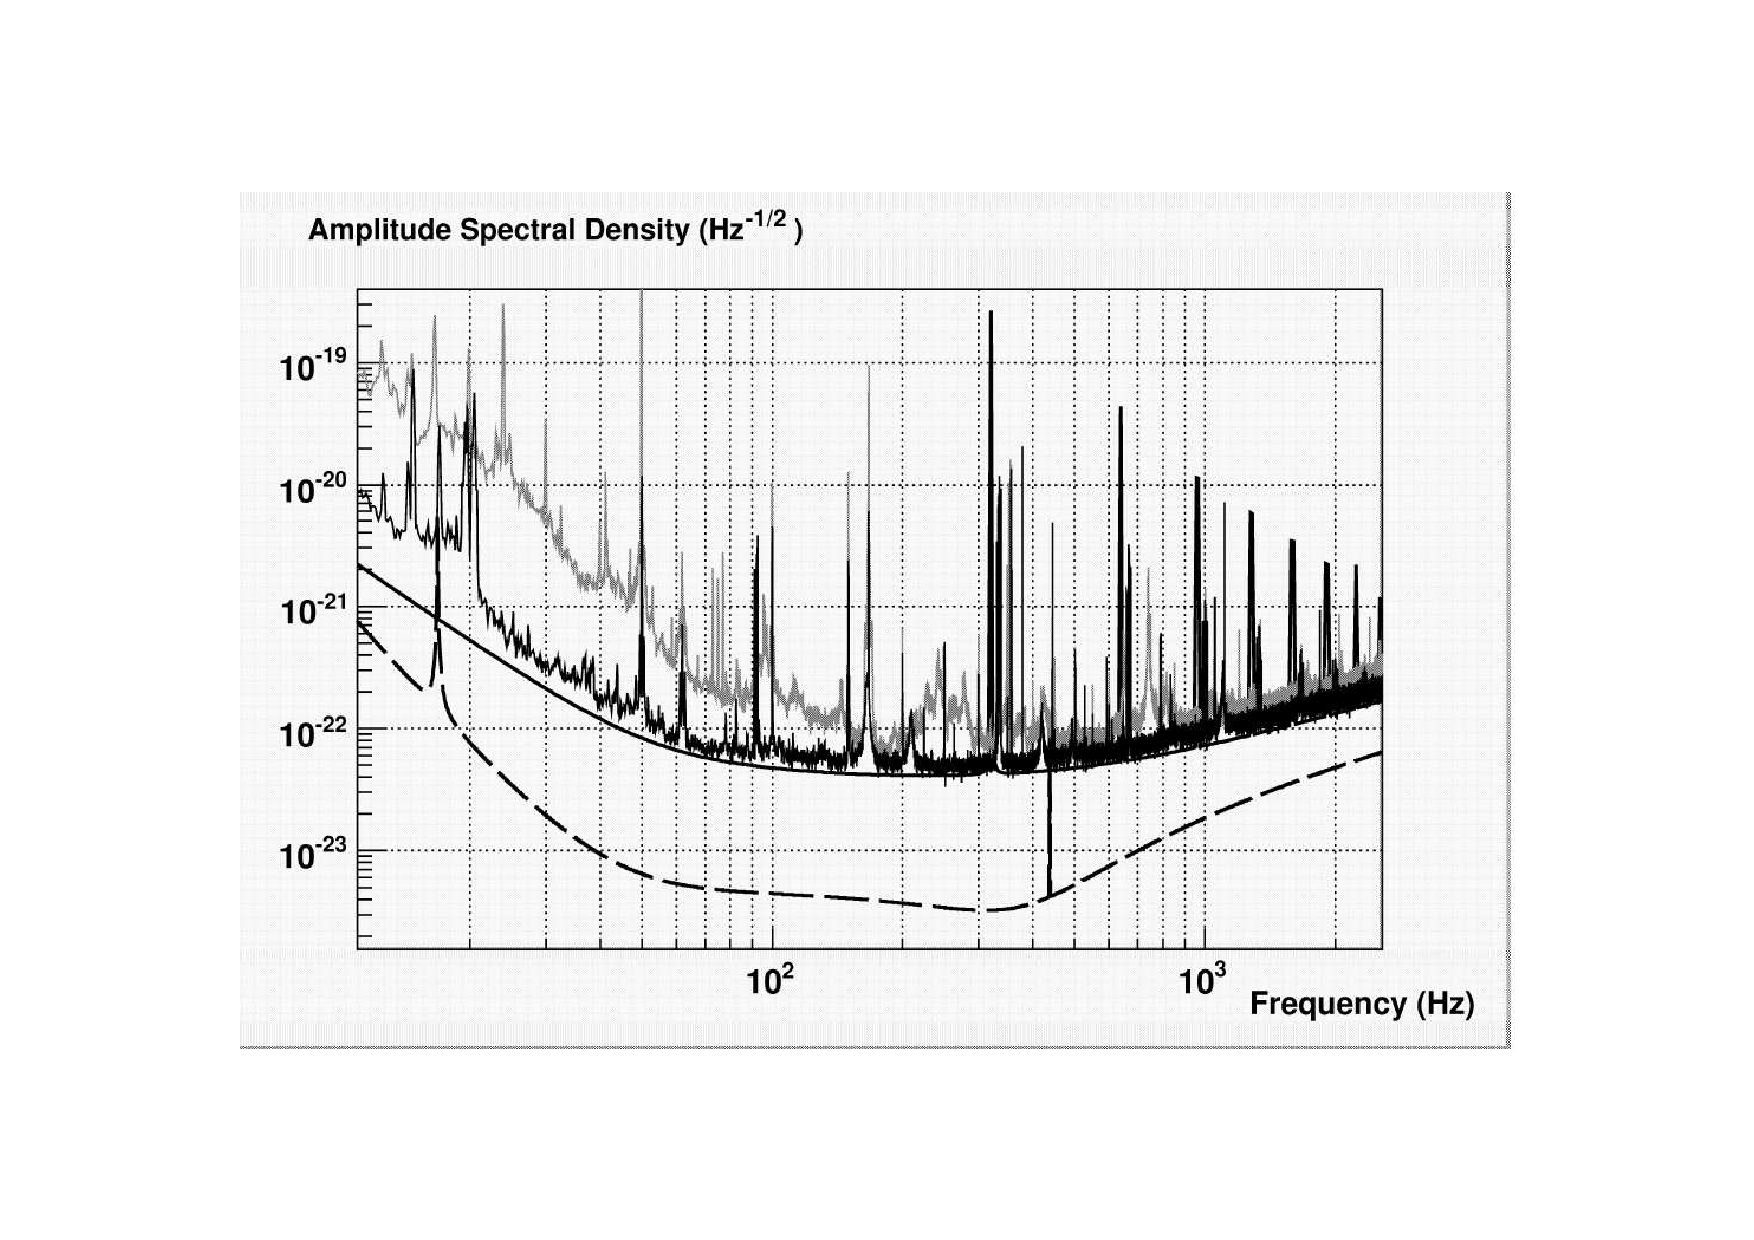
\includegraphics[width=18cm]{./Sec_Suspensions/Figures/Fig1.pdf}
			\caption{Virgo sensitivity achieved after a few months of the second   scientific run (\emph{VSR2} - black experimental curve), compared with the sensitivity reached in 2007 during the first scientific run (\emph{VSR1} - grey curve). The continuous curve is the Virgo design sensitivity, discussed in \cite{Punturo2004}, while the dotted curve is the design sensitivity of Advanced Virgo, the next generation detector.}
\label{FigSusp1}
	\end{center}
\end{figure}
%
\begin{figure}[t!]
	\begin{center}
		 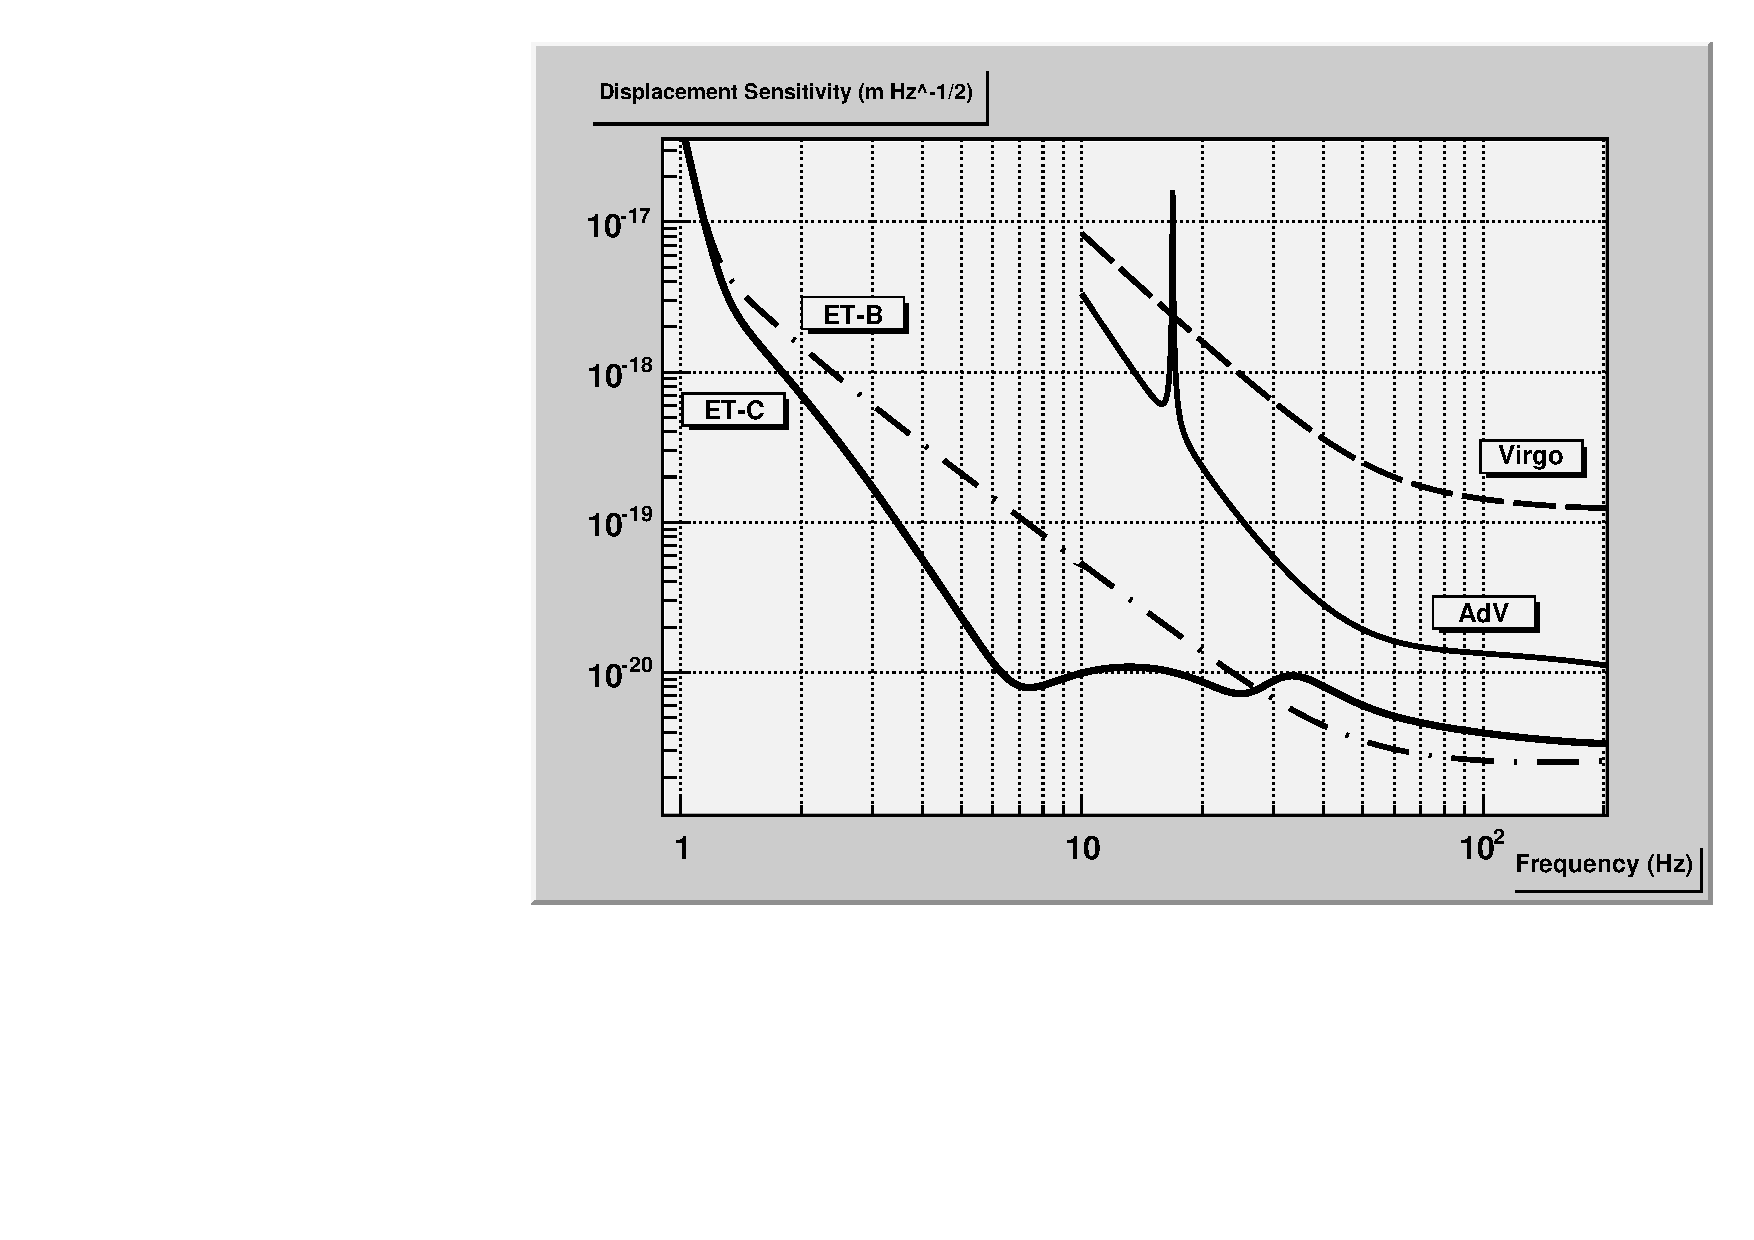
\includegraphics[width=16cm]{./Sec_Suspensions/Figures/Fig2.pdf}
			\caption{Displacement design sensitivities of Virgo, Advanced Virgo~(AdV), and of the two reference configurations of the Einstein Telescope: the high-frequency interferometer (ET-B) and the `xylophone' design (ET-C), optimized for the low frequency detection. While the detection bandwidth of Virgo and AdV starts from 10 Hz, Einstein Telescope aims to extend the detection bandwidth in the low frequency region starting from a few Hz.}
\label{FigSusp2}
	\end{center}
\end{figure}
%
\begin{figure}[t!]
	\begin{center}
		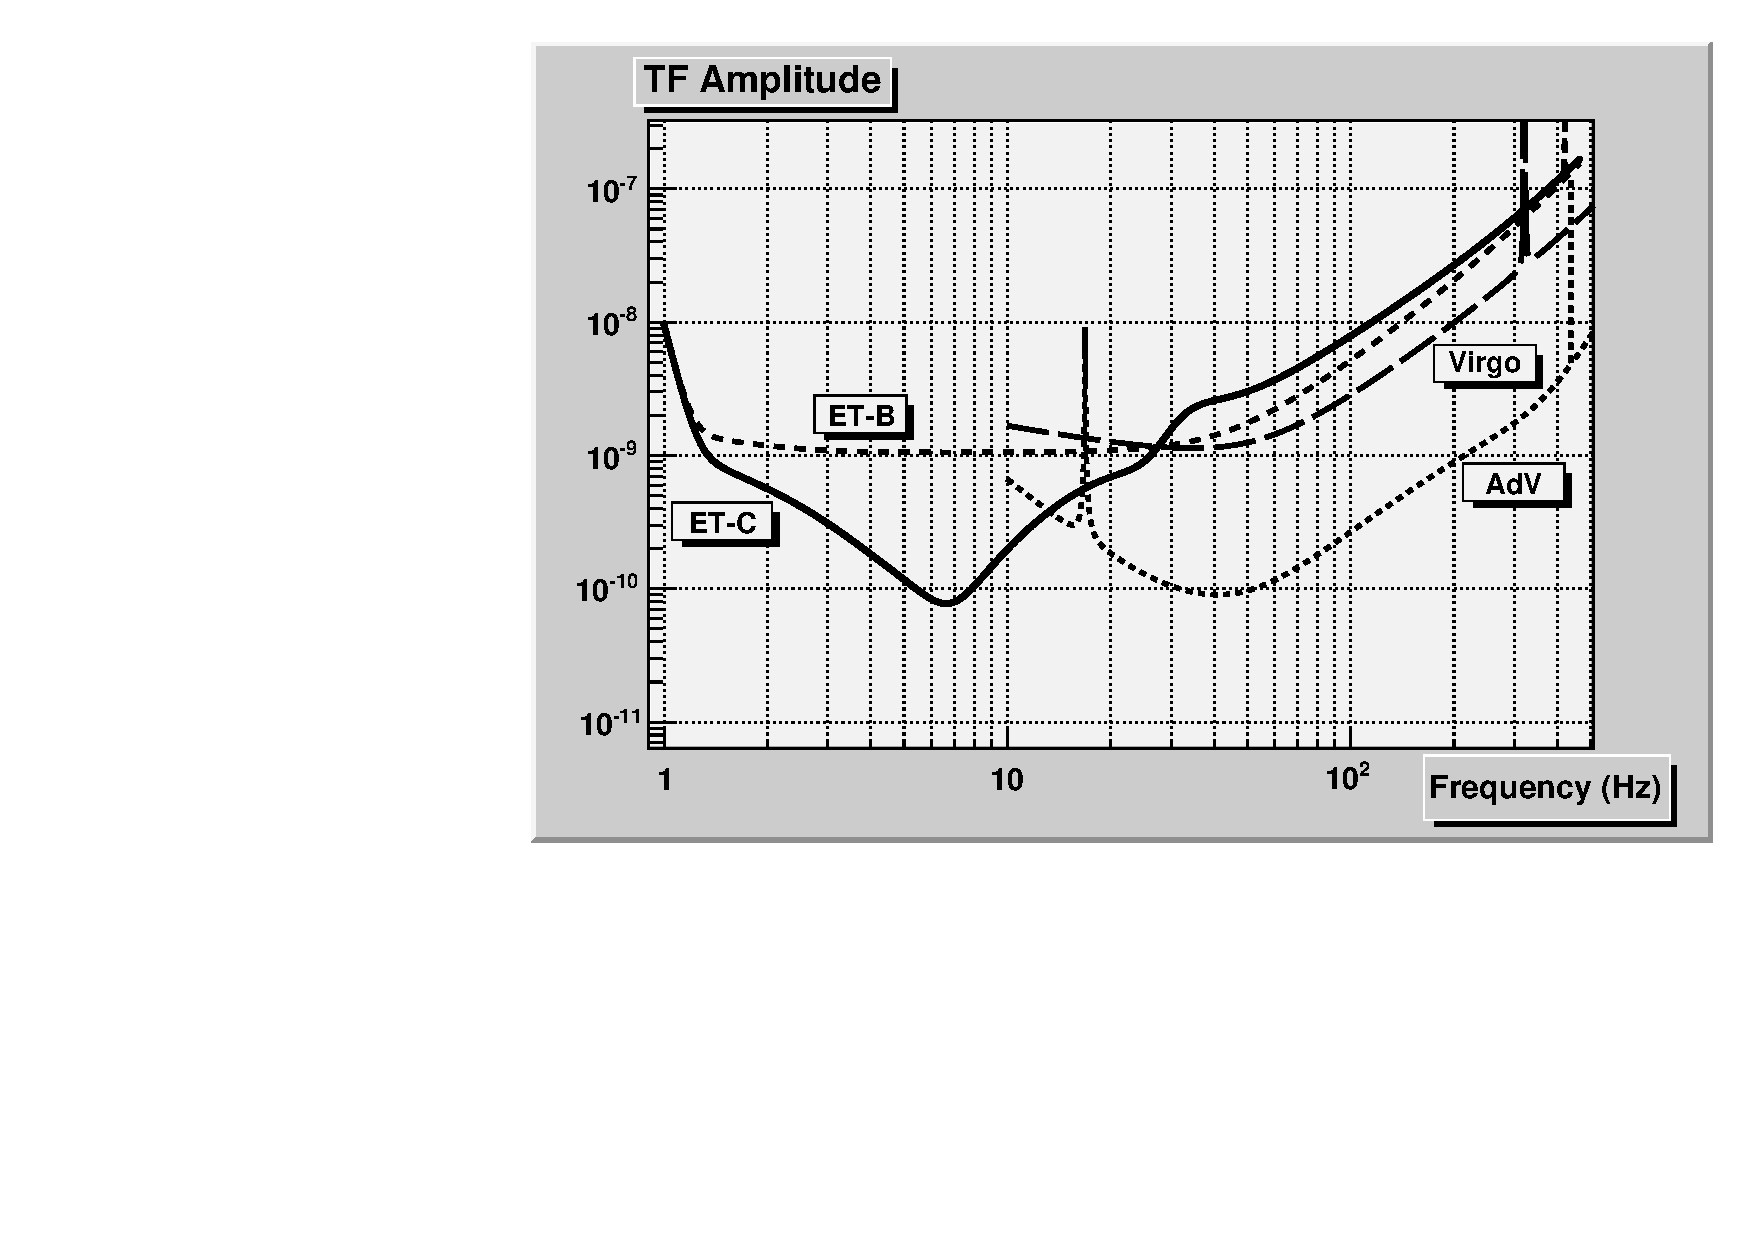
\includegraphics[width=16cm]{./Sec_Suspensions/Figures/Fig3.pdf}
			\caption{Seismic vibration transfer function requirements for different antennas. The curves represent the ratio between the displacement sensitivities reported in figure~\ref{FigSusp2} and the conservative linear spectral density of seismic noise at the level where the interferometer is located. Since seismic noise will be at least a couple of orders of magnitude smaller in underground environment, Einstein Telescope, despite its better sensitivity, is less demanding in terms of seismic attenuation at high frequency.}
\label{FigSusp3}
	\end{center}
\end{figure}
%
The maximum acceptable transfer function amplitude of the seismic isolation system in different antennas is plotted as a function of the frequency in figure~\ref{FigSusp3}. This is given by the ratio between the detector displacement sensitivity curves reported in figure~\ref{FigSusp2} and the linear spectral density of seismic noise measured on site at ground level. At the Advanced Virgo site (the same of Virgo) the linear spectral density of the ground seismic displacement has been measured to be roughly isotropic and well approximated, between a fraction of Hz and a few tens of Hz, by the function $A/f^{2}$, where $f$ indicates the spectral frequency and $A$ is around $10^{-7}\,\mathrm{m\cdot Hz^{3/2}}$~\cite{Acernese2004}. A conservative value of $A$ around $5\times10^{-7}\,\mathrm{m\cdot Hz^{3/2}}$ has been considered to take into account possible fluctuations in some spectral regions, and the fact that the residual displacement due to seismic noise affects all four mirrors of the two Fabry-Perot cavities. Since the Einstein Telescope site has not yet been chosen, the requirement has to be considered as provisional. The linear spectral density seismic noise of $5\times 10^{-9}/f^{2}$, measured in the Kamioka mine, where the new cryogenic Japanese interferometric detector is planned to be installed~\cite{Ohashi2003July31-August7}, is taken as a reference value. The recent progresses of Einstein Telescope working group for site selection are promising~\cite{Beker2009}. In particular, a measurements campaign of seismic noise for different underground sites in Germany provides seismic spectra smaller by a few units or comparable with that one measured in Kamioka mine. This makes the chosen reference seismic floor conservative for our goals (the requirements are likely more stringent than necessary).

It is important to stress that the transfer function requirements are valid both for vertical and horizontal seismic noise, that have a similar magnitudes. While for horizontal direction the argument is straightforward, in the vertical case the plot represents the maximum fraction of vertical seismic noise that can be transferred to the mirror along the beam direction without affecting the antenna sensitivity. As shown in the following section, only a fraction of the mirror vertical motion is transmitted along the beam because of unavoidable mechanical coupling and Earth curvature (making 10\,km far plumb lines \footnote{A plumb line is  regarded as directed exactly toward the earth's center of gravity.} not parallel each other). 

\paragraph{b) The Virgo Superattenuator (SA)}

Since it will be shown that the \emph{Superattenuator} as it is operating within the Virgo interferometer is already compliant with the ET project requirements above 3\,Hz, it is important to provide a detailed description of the apparatus.
The \emph{Superattenuator} working principle is based on a simple idea. Exciting in horizontal direction the suspension point of a simple pendulum at frequency $f$ higher than the pendulum normal mode $f_0$, it is easy to prove that the oscillation is transmitted to the suspended mass with an attenuation proportional to $(f_0/f)^{2}$. Therefore a device suspending a mirror based on the working principle of a simple pendulum, represents a good isolation system for seismic noise at frequency $f > f_0$.
A better attenuation performance is achievable considering a \emph{n-stage} pendulum. With this system an oscillation at a frequency $f$ higher than the frequencies of the chain normal modes $(f>f_0>f_1> \ldots >f_n)$, is transmitted to the suspended mass with attenuation proportional to $f^{-2n}$. In particular, the ratio between the linear spectral density of the last mass displacement (the optical component) and the linear spectral density of the suspension point displacement (where the excitation is applied), decreases as $A/f^{2n}$ where 
$A=f_0^{2}\cdot f_1^{2} \cdot f_2^{2} \cdots f_n^{2}$ and $n$ is the number of stages. In this way a very large attenuation of seismic noise horizontal component can be obtained in the frequency range above the highest pendulum resonance, simply increasing the number of stages. The longer are the pendulums, the lower are the resonant frequencies of the system and higher is the attenuation response at a given frequency.

Unfortunately, due to different directions of the plumb line on the curved Earth surface, the end mirrors, suspended 3\,km away in the Virgo interferometer and 10\,km in Einstein Telescope, are misaligned (each with respect to the other) by about $3\times 10^{-4}$\,rad and $10\times 10^{-4}$\,rad respectively. For this reason it is necessary to tilt one mirror with respect to the other by the same amount, making at least one mirror misaligned with respect to the local plumb line. With this setting up the mirrors are not perfectly perpendicular to the laser beam and then any vertical vibration will be partially transmitted to the interferometer horizontal axis (laser beam direction). In addition any vertical vibration will be partially transmitted to the interferometer horizontal axis because of an unavoidable coupling among different degrees of freedom. Thus vertical motion will cause a phase change of the laser beam. It is thus clear that a vertical attenuation of seismic noise comparable with the horizontal one is fundamental to reduce the observation frequency threshold. With a multistage pendulum this goal can be achieved by replacing each suspension wire with a spring to form a cascade of oscillators also along the vertical direction. The spring should support a heavy load and, at the same time, it should be soft enough to exhibit a low resonant frequency. With this technical solution it is possible to confine the vertical resonances of the chain in a low frequency range obtaining a strong attenuation starting from a few Hz. 

Even the unavoidable mechanical couplings between rotations and horizontal beam direction can cause a phase change on the interferometer laser beam. In order to confine these rotational mode frequencies well below the detection band, each pendulum mass has to be replaced by a structure having a high momentum of inertia. In addition, the diameter of the suspension wire, connecting two consecutive stages, has to be small enough to reduce its restoring torque which opposes the rotation of the chain and determining its rotational frequencies. An interconnection of the stages at small distance and as close as possible to their centres of mass, guarantees low frequency tilt modes (i.e.\ rotational modes around the two horizontal axes) and a negligible coupling effects on the horizontal displacement of the suspended mass.

Keeping in mind all the considerations reported above, the Virgo \emph{Superattenuator} has been conceived having a mechanical structure based on the working principle of a multistage pendulum~\cite{Ballardin2001}. Each mirror, indeed, is suspended to a 8\,m-long SA chain with 6 mechanical filters (see Fig.~\ref{SAfig1}). The system consists of three fundamental elements: the Inverted Pendulum (\emph{IP}), the mechanical seismic Filters (\emph{SF}) connected each other by metallic suspension wires and the Last Stage (\emph{LS}) or optical payload. The suspension system is described here below, while more detailed information of each single chain element can be found in reference~\cite{TheVirgoCollaboration1995}.

\begin{figure}[t]
	\begin{center}
		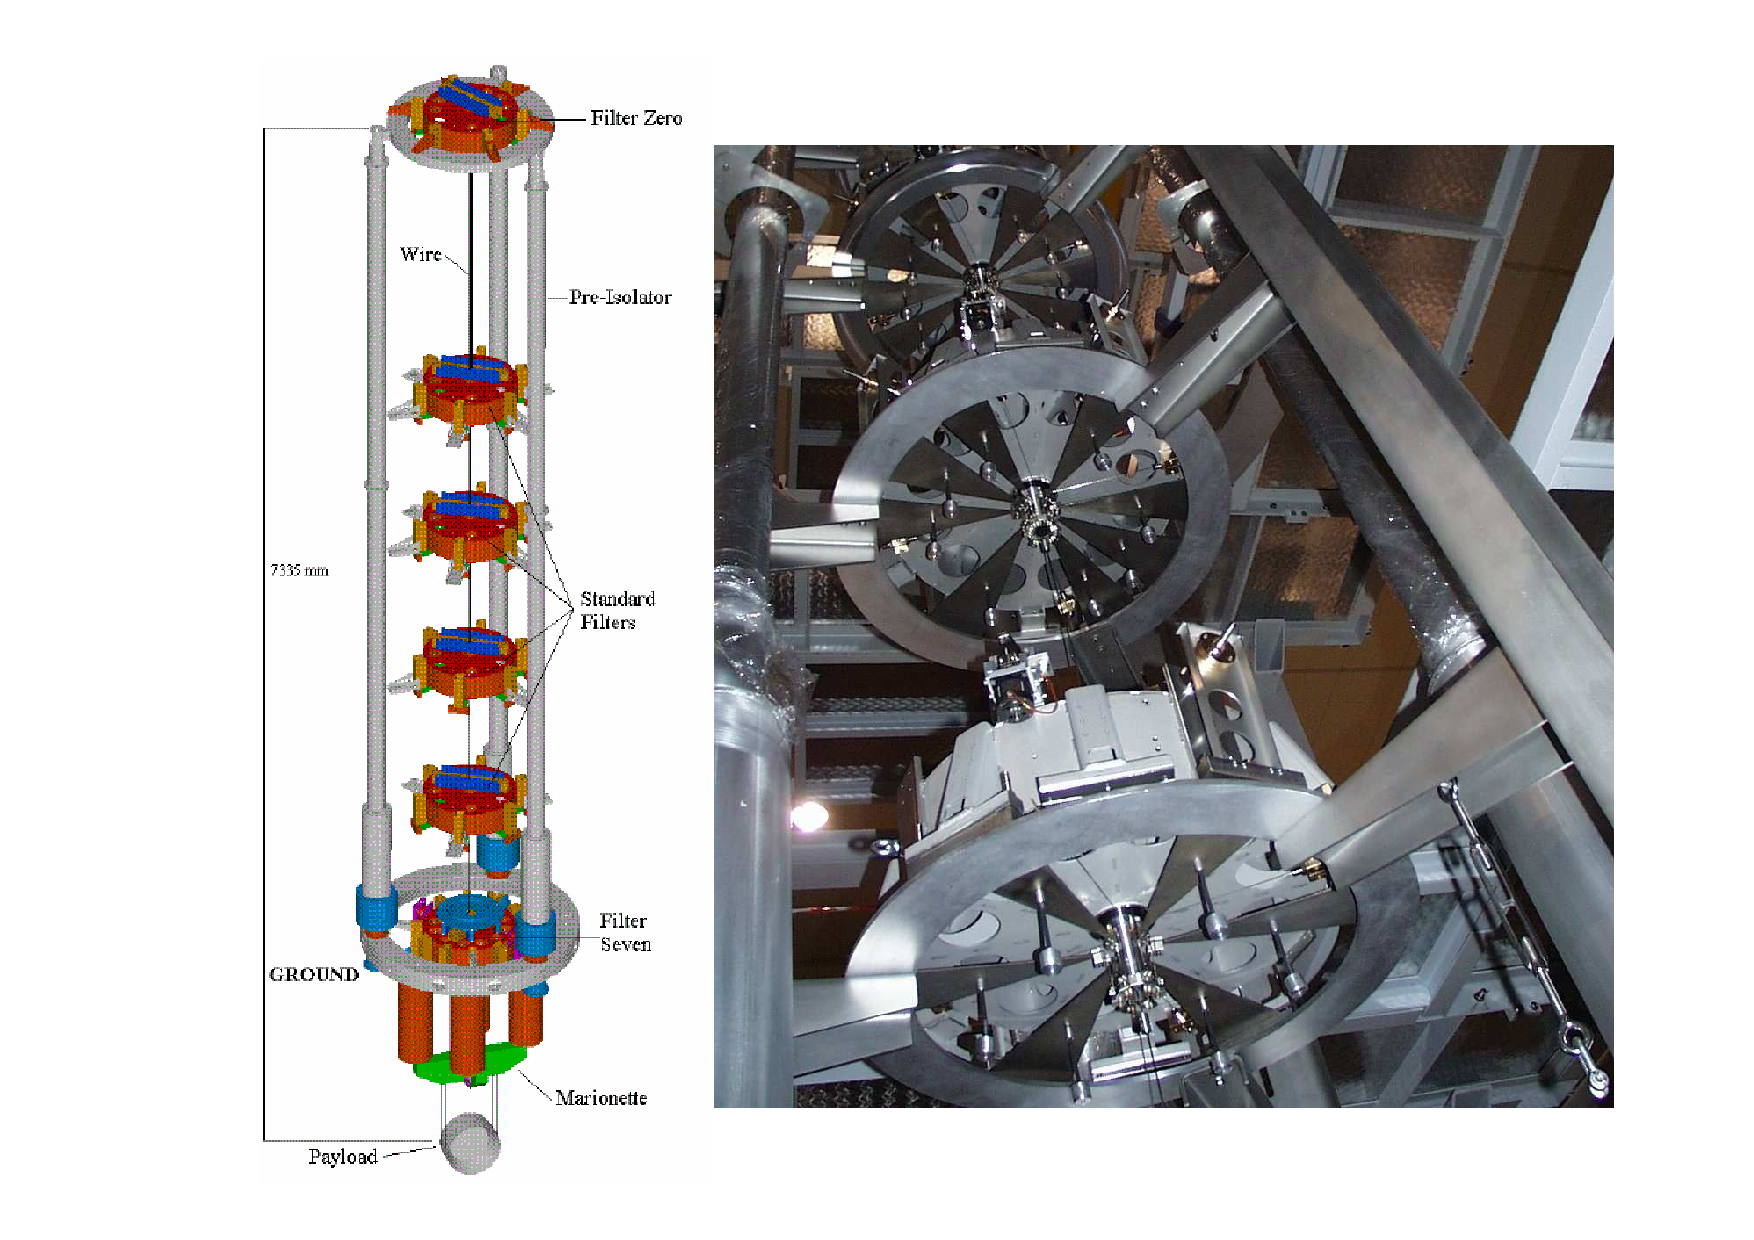
\includegraphics[width=17cm]{./Sec_Suspensions/Figures/SAfig1.pdf}
			\caption{The Virgo \emph{Superattenuator} suppresses the transmission of ground seismic vibrations to the suspended mirror. The mechanical filter chain and the three legs of the inverted pendulum are visible. In our attenuation measurements the excitation is applied to the filter chain suspension point.}
\label{SAfig1}
	\end{center}
\end{figure}

\subparagraph{The Inverted Pendulum top stage}
The top stage of the \emph{Superattenuator} is designed to fulfil three main functions:
\begin{itemize}
\item to introduce a very low frequency (about 40\,mHz) horizontal filtering stage, limiting the amount of seismic energy feeding into the SA and thus reducing the SA excitation resonant modes and improving its overall attenuation performance;
\item to provide the SA with a suspension point positioning system: the amplitude of the slow tidal drifts over three km is far beyond the dynamic range of the actuators exerting the locking forces upon the mirror. Therefore tidal drifts are compensated by moving softly the SA suspension point: the tidal strain over 3\,km can be as large as a few hundred microns in 6 hours;
\item to provide a soft suspension stage on the top of the chain to allow active mode damping of the chain resonant modes and seismic noise depression by means of inertial sensors, positioning sensors and electromagnetic actuators. The main goal is to reduce the \emph{swing} of the optical payload down to a fraction of micron allowing a low-noise control of the mirror in the interferometer.
\end{itemize}
To fulfil all the above requirements in the horizontal plane a device based on the working principle of an Inverted Pendulum (\emph{IP}) has been built. An IP is a suitable device for several reasons. An ideal Inverted Pendulum can be conceived as a mass-less vertical bar of length~$l$ connected to ground by means of an elastic joint with stiffness~$k$ and supporting a mass~$M$ on its top. In such a pendulum the gravity acts as an anti-spring and the resonant frequency can be tuned to have a very low resonant frequency (about 40\,mHz in Virgo). The required force to displace the suspended chain from an IP resonating at 40\,mHz is very low: the needed force, in DC mode, for moving a 1\,ton SA chain by 1\,cm is less than 1\,N. Therefore soft electromagnetic actuators can be used to control the mirror position. For this reason the IP is a good platform to act upon for the active damping of the SA normal modes.

The present Virgo Inverted Pendulum (see Fig.~\ref{SAfig1} left side) is a three-leg metallic structure interconnected on their top with a steel ring (the Top Ring). The Top Ring surrounds the first filter of the chain (hereafter called Filter Zero) to which is rigidly connected. The Filter Zero together with the Top Ring form a platform suspended by three thin wires (31\,mm long) accommodated on top of the legs. The elasticity of the structure is due to three flexible metallic joints. They are screwed onto the legs to form an interconnection element between the upper part and the bottom one of the aluminium pipes. A bottom steel ring, on which the Inverted Pendulum is anchored, completes this metallic frame. 
Each leg is essentially a light hollow cylinder made of aluminium with an inner diameter of 125\,mm and an outer diameter of 130\,mm. The total length of the leg, from the bottom of the flexible joint to the suspension point of the SA is about 6.2\,m. The leg is composed by two sections flanged together and reinforced with titanium inserts. 

The three legs are made in Aluminium to minimize their weight. Nevertheless the leg mass is about 26\,kg. An extension below the flex joint is necessary to tune the \emph{percussion} \emph{point} avoiding an isolation performance spoiling. The flex joint is therefore mounted on top of a 0.8\,m high rigid support. A proper counterweight is attached to a high bell-shaped 0.9\,m long skirt bolted to the bottom of the leg.

The Inverted Pendulum structure is surrounded by a rigid metallic frame (called Ground Reference Structure---visible in Fig.~\ref{SAfig1} right side), holding the parts of sensors and actuators that needs to stay ``on ground''. It is provided with~\cite{Losurdo1999,Losurdo2001}:
\begin{itemize}
\item three motorized sleds set on the external structure in front of the legs top. Each sled is connected to the corresponding leg top through a soft spring. The motors are used to set the IP roughly in its working point, so that to minimize the correction signals in the closed loop operation; 
\item 3 horizontal \emph{LVDT} position sensors set in pin wheel configuration. The secondary windings stay on the ground reference structure, while the primary ones are rigidly connected to the top stage;
\item 3 horizontal coil-magnet actuators, set in pin wheel configuration. The coils, arranged as a Maxwell pair, stay on the ground reference structure, while the magnets are rigidly connected to the top stage;
\item 3 horizontal accelerometers, set on the top stage;
\item 2 vertical accelerometer, set on the Filter Zero crossbar;
\item 1 vertical \emph{LVDT}, measuring the position of the Filter Zero crossbar with respect to the top stage;
\item 2 vertical coil-magnet actuators, acting between the Filter Zero body and its crossbar.
\end{itemize}
%%
\begin{figure}[t]
	\begin{center}
		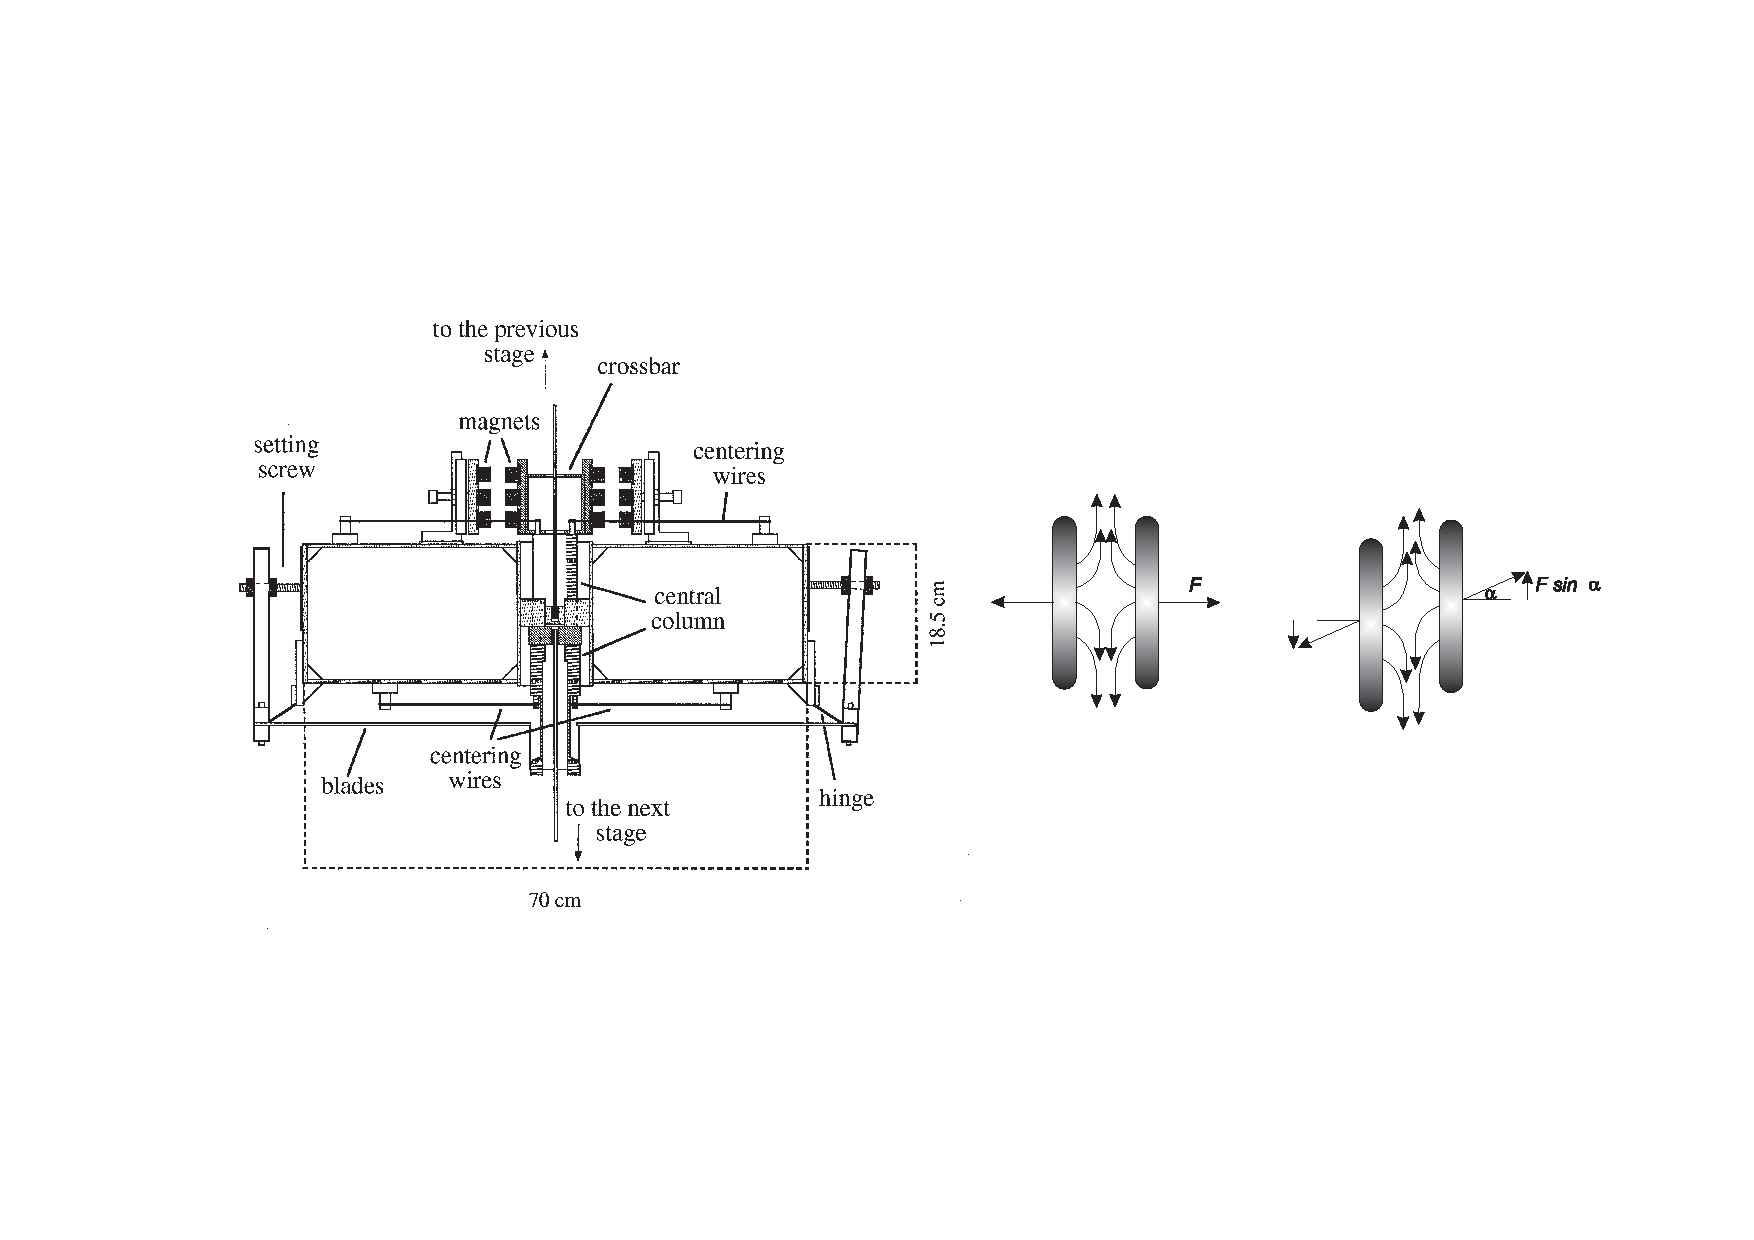
\includegraphics[width=17cm]{./Sec_Suspensions/Figures/SAfig2.pdf}
			\caption{The Virgo seismic filter: a technical drawing (\emph{left side}). The working principle of the magnetic anti-spring system accommodated on the seismic filter crossbar (\emph{right side}).}
\label{SAfig2}
	\end{center}
\end{figure}
%%

\subparagraph{The Seismic Filters}
In the Virgo \emph{Superattenuator} each pendulum mass has been replaced by a rigid metallic structure drum shaped acting as an oscillator in vertical direction too. A sequence of six mechanical filters is able to isolate the optical components from seismic noise in accordance with the working principle of a multistage pendulum (see Fig.~\ref{SAfig1}). A detailed description of the design and performance of a single filter can be found in reference~\cite{Beccaria1997}. A seismic filter is a rigid steel cylinder (70\,cm diameter, 18.5\,cm high for a total weight of about 100\,kg) suspended as close as possible to its centre of mass (see Fig.~\ref{SAfig2} left side). On the outer circumference of its body bottom part, a set of triangular cantilever spring blades is clamped. Each blade (3.5\,mm thick and 385.5\,mm long) is bent at a constant curvature radius and with different base width according to the load to be supported. A nominal load, ranging between 48\,kg and 96\,kg hung on the blade tip, forces it in flat and horizontal position. The blade tip is connected by a 1\,mm diameter wire to a central column, inserted through a hole in the centre of the filter body. Any movement of the central column, apart from the vertical direction, is prevented by two sets of four centreing wires accommodated on the top and on the bottom of the filter body.

A crossbar, bolted on the upper part of the central column, is used as a mechanical support for the magnetic anti-spring system described in the next sub-paragraph. The central column and the crossbar, connected to the blade spring, represent the moving part of the mechanical filter from which the load of the lower stages is suspended by a steel suspension wire. By connecting each filter to the next one, a chain of mechanical oscillators in vertical direction is obtained.

According to the previous description of our filtering system it is clear that the total load of the chain is suspended by the triangular steel blades. The base width of the triangle ranges from 180 to 110\,mm in accordance with the load to be supported. For the same reason the top filter is equipped with 12 blades while the last one needs only four blades.Once properly loaded the main vertical resonant frequency of each filter is about 1.5\,Hz. 

Maraging steel has been used in place of standard steel for blade construction in order to minimize micro-creep effects~\cite{Beccaria1998,Braccini2000} due to the high load applied. The same material has been used to machine the suspension wires with nail-head at both ends~\cite{Delapierre1997}. Since the suspended load decreases going from the top to the bottom of the chain, the wire and the nail-head diameters change along the chain in the ranges 4--1.85\,mm and 8--6\,mm, respectively. In this way it has been possible to confine the violin vibration mode within the high frequency band and to reduce its angular stiffness which determines the rotational frequency around the vertical axis. 

The two nail-heads of the wires connecting a filter on the chain to the previous and to the next one are screwed in the central part of its body at a relative distance of 5\,mm, very close to the filter centre of mass. As mentioned above, this guarantees a small return torque to rotations of the filter around the horizontal axis and thus a low tilt frequency.

\subparagraph{The magnetic anti-spring}
The suspension wire length of 1.15\,m in the Virgo \emph{Superattenuator} sets the pendulum resonant frequency of each stage at about 0.5\,Hz. In the vertical direction the stiffness of the triangular blade springs fixes the natural resonant frequency at about 1.5\,Hz. In order to reduce the vertical stiffness of the blades, and then to confine the main vertical resonant frequency of each filter below the pendulum one, a system of magnetic anti-springs \cite{Beccaria1997,Braccini1993} has been adopted (see Fig.~\ref{SAfig2} left side). It consists of two sets of permanent magnets (the first assembled on the crossbar and the second one on the filter body), facing each other with opposite horizontal magnetic moment (namely in a repulsive configuration). In this way the two matrices screwed on the crossbar are forced to move in vertical direction only. 

When the magnets are perfectly faced the repulsive force has a null vertical component, but as soon as a matrix is moved in the vertical direction, a vertical component of the magnetic force appears. Considering a small relative displacement ($\Delta{y}$), compared with the distance ($d$) between two matrices of magnets and with their transverse dimension, the vertical component of the repulsive force ($F_y$) is proportional to $\Delta{y}$:

\beq
F_{y}\approx F_{0}\cdot (\Delta y/d)
\label{mag}
\eeq

where $F_0$ is the modulus of the repulsive force (see its working principle in Fig.~\ref{SAfig2} right side). Such device is equivalent to a vertical spring with a negative elastic constant (anti-spring) whose modulus is $F_0/d$. Thus, its rest position is that of  the two couple of matrices perfectly faced. On a seismic filter the magnetic anti-springs act on the crossbar in parallel with the blade springs, so that the vertical modes frequency of the chain are confined below the highest frequency of the horizontal ones. 
The advantages of this system are the vacuum compatibility and the contact-less
action performed on the filter, for this reasons it represents the reference solution for the third generation detector.

An evolution of the Virgo mechanical filter to be used as vertical seismic noise  
suppression system, is the Geometric Anti Spring (GAS) filter described in the appendix \ref{sec:Gas_spring}. It was proposed  by R. De Salvo et al.~\cite{cella} few years ago and it has been tested in TAMA. 
The GAS filter is used as seismic isolation system for the 10 m 
long interferometer at AEI Hannover and the same technology is developed by the NIKHEF group for the optical bench of the light injection in the interferometer for Advanced Virgo.


\subparagraph{The Steering Filter} \label{steeringF}

The last mechanical filter of the Virgo seismic attenuation chain is the Steering Filter~\cite{Ballardin2001}. It has been designed to suspend and orientate the payload, a multi-body mechanical system whose core is a test-mas of the gravitational-wave detector, by means of forces exerted within the suspension. The payload plays a crucial role in the overall dynamics 
of the system and its presence has been included in all the projections shown in this section of the report, assuming a basic design similar to that one actually developed for Virgo (Fig.~\ref{SAfig1}). However a dedicated section~\ref{sec:last_stage} will be devoted to the issues related to this 
system provided its crucial role in dealing with test-masses as mirrors of the interferometer. In the Virgo experimental apparatus the steering filter has been equipped with four Aluminium legs (about 900\,mm long and 250\,mm in diameter) bolted on the filter body bottom part. These legs are the mechanical support of the coils mounted in front of the permanent magnets screwed on the marionette wings and used to control the payload position.

In addition the Steering Filter is equipped with different vacuum compatible stepping motors. Two of them are dedicated to the filter alignment around its vertical axis. The first one is accommodated on top of the filter body and it is used to move the filter and the payload with respect to the upper part of the \emph{Superattenuator} while the second one is mounted at the bottom of it to change the relative position of the filter with respect to the payload. This last one is used to optimize the coil-magnet distance for the actuation on payload. A second pair of vacuum compatible stepping motors completes 
a set of remote controlled devices mounted on this mechanical filter. By moving some small masses attached to a mechanical trolley on top of the filter body, a fine adjustment of the tilt (rotations around the two horizontal axes) can be performed. 


\paragraph{c) Seismic isolation measurements with the Superattenuator (SA)}

The attenuation performance of the \emph{Superattenuator} has been measured by using the Virgo interferometer. In particular, a direct measurement of the mechanical transfer function has been obtained exciting with sinusoidal forces the top stage of  the mechanical filter chain. The measurement consists in detecting the presence of a spectral line with the same excitation frequency at the level of the mirror, i.e.\ at the interferometer dark port. The ratio between the linear spectral density at the excitation frequency of the mirror and that one of the top stage displacement (measured by means of the accelerometers) provides a measurement of the \emph{Superattenuator} mechanical transfer function magnitude. When the line is not detected at the level of the interferometer, only an experimental upper limit of the transfer function amplitude can be given. We remind that the linear spectral density of the noise floor of the top stage sensors or of the interferometer dark port, does not depend on the time length of the measurement while the amplitude of a spectral line increases with square root of the time interval. The longer is the integration time, the higher is the capability to distinguish a spectral line from the interferometer noise floor. Moreover, in those measurements where the peak is not distinguished at the level of the mirror, the upper limit of the transfer function, given by the ratio between the noise spectral floor and the top stage peak at the excitation frequency, improves (i.e.\ becomes smaller) increasing the integration time. In this case, the linear spectral density of the excitation line (denominator) becomes larger, while the interferometer noise floor (numerator) does not change.

A campaign of measurements has been performed exciting the suspension top stage both in horizontal laser beam direction and in vertical direction. The excitation is applied to the suspension point through the coil-magnet actuators used in the Inertial Damping of the chain resonance modes. The experimental results have been compared with the requirements of the future generation detectors (as reported also in Fig.~\ref{FigSusp3}) and plotted in Fig.~\ref{FigSusp5}.

\begin{figure}[t]
	\begin{center}
		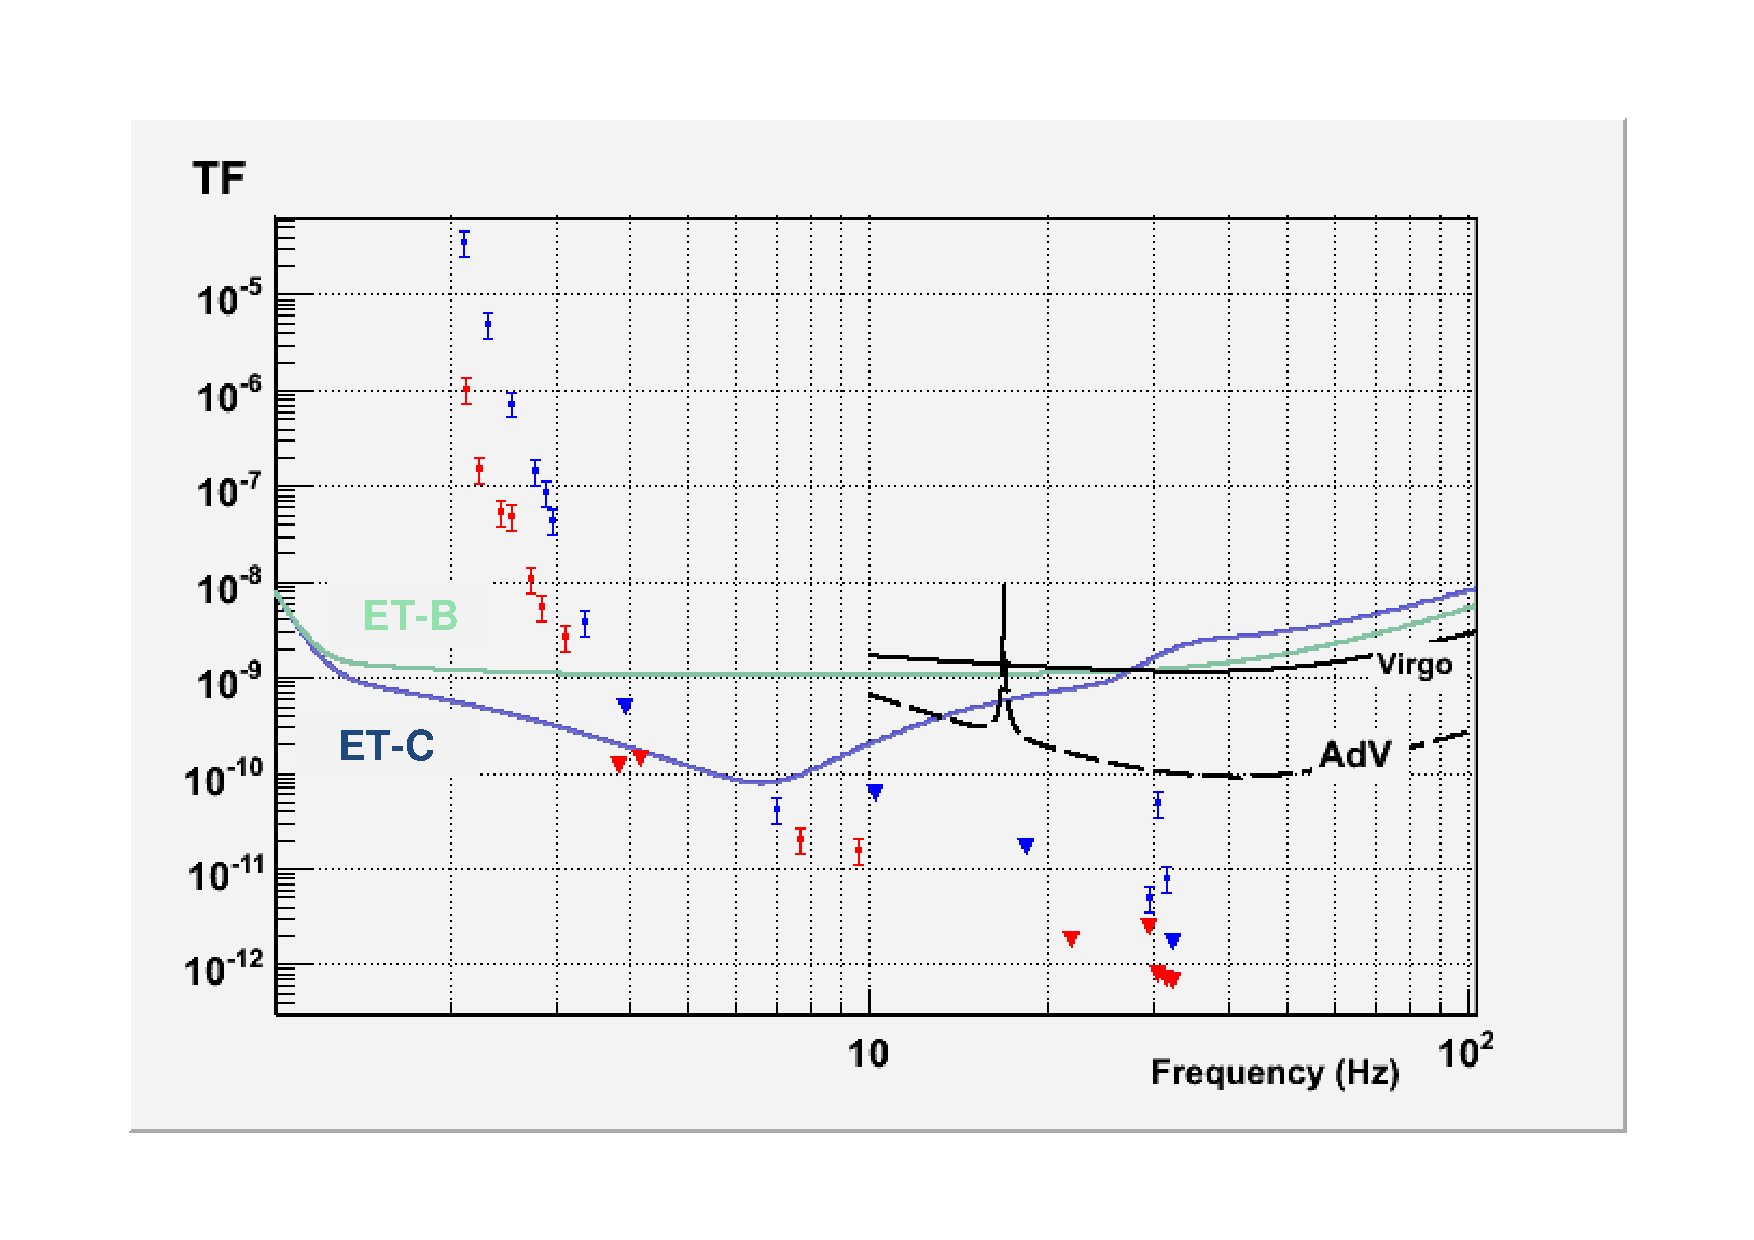
\includegraphics[width=0.9\textwidth]{./Sec_Suspensions/Figures/Fig5.pdf}
			\caption{The measurement of the transfer functions at different frequencies. In red are reported the measurements where a vertical excitation of the top stage is applied. In blue are the measurements with the excitation in horizontal direction. The upper limits are indicated by triangles, while the direct measurements (when a signal is detected at the level of the mirror) are indicated with the bars. For the discussion of the error bars see reference~\cite{Collaboration2010}.}
\label{FigSusp5}
	\end{center}
\end{figure}

Above 3 Hz all the measured transfer functions (upper limits or direct measurements) turn out to be within the requirements of Einstein Telescope. Changes to the \emph{Superattenuator} structure (such as a length extension of the filter chain) will be needed in Einstein Telescope only in the case the detection threshold frequency will be moved below 3 Hz. In reference \cite{Ballardin2001}, where a stage by stage (indirect) measurement of the \emph{Superattenuator} total transfer function (valid at any frequency) has been provided (and compared with simulation), a very steep behavior around 3 Hz is well visible. Considering this as a reference result, it is clear that even changing by a couple of orders of magnitude the input seismic noise as well as the attenuation requirements, the crossing frequency between the transfer function and the requirement curve should remain around 3 Hz. 

In addition, around 30 Hz and in the 7-9 Hz region, our measurements put in evidence some peaks above the interferometer noise floor while excitation is applied on the top stage. This is an indication of noise transmission a couple of orders of magnitude larger than expected from simulation and indirect measurements (stage by stage). However, also in these cases, the transfer function has been measured to not exceed the detector requirements. Other mechanisms could cause the detected tiny motion of the mirror by-passing the extremely high mechanical attenuation, as discussed in \cite{Collaboration2010, Braccini2010March1-3}. The extension of the multistage pendulum length, linked to the need of moving down below 2 Hz the cross-over between the horizontal seismic noise and the antenna sensitivity (see next section), is welcome for a better separation of the top-stage control and the optical payload control preventing cross-talks.

It is important to stress that, during our measurements campaign, the pre-isolator stage (described above) has been excluded from the transfer functions measurements. So that an additional attenuation factor, of the order of 20--40\,dB, has to be considered as safety margin. With this additional attenuation factor, one can conclude that the cross-over for the Einstein Telescope requirements is expected to be around 2.8\,Hz by using the present \emph{Superattenuator} scheme. The cross-over is dominated by horizontal seismic noise.


\paragraph{d) SA modifications for Low Frequency ET}

In order to extend the detection bandwidth of the Einstein Telescope in the low-frequency region starting from a couple of Hz, a better seismic attenuation in the ultra-low frequency range is needed. To this purpose a detailed simulation campaign devoted to this design study has been performed. The SA dynamics in the low frequency range, where the inner normal modes of the mechanical filter chain are confined, can be well simulated by using the electro-magnetic equivalent circuit (a series of oscillators). 
A maximization algorithm, called \emph{Simplex}~\cite{Different2008_SecondEdition}, based on the possibility to change the masses and the mechanical filter chain lengths, has been developed. It searches for a maximum attenuation performance at a fixed frequency that, in our case, was 2\,Hz.  Since the transfer function has a smooth shape, it turns out that to get a higher attenuation at 2\,Hz, we should have a lower  "cross-over frequency" with the requirements curves (see Fig.~\ref{Par4Fig1}). As showed in the direct measurement performed with the Virgo interferometer (see section 4.1.1.c), the cross-over between seismic noise at the mirror level and the requirements is dominated by the residual horizontal seismic vibrations. For this reason to move the cross-over at lower frequency, we need to improve  the attenuation performance of the horizontal seismic vibration in the low frequency range.
%
\begin{figure}[t]
	\begin{center}
		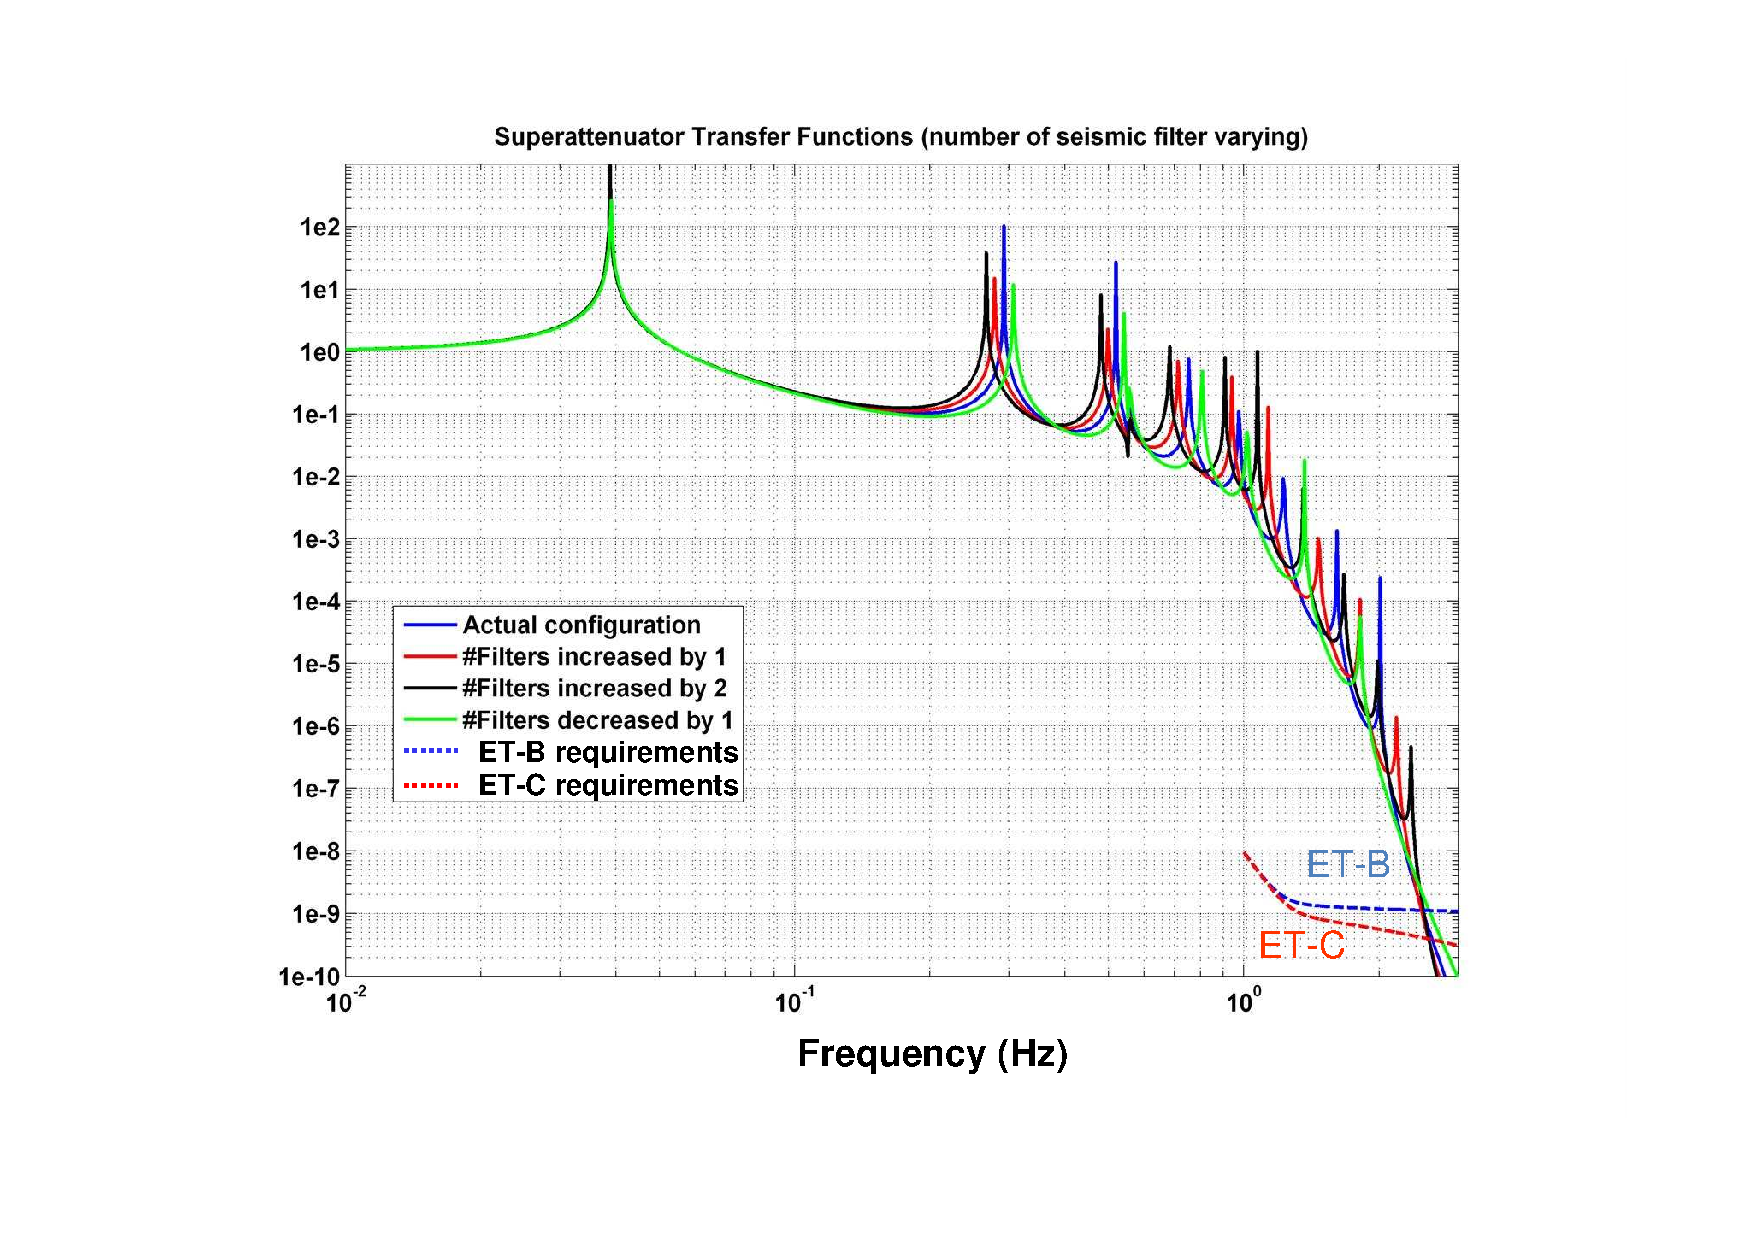
\includegraphics[width=0.9\textwidth]{./Sec_Suspensions/Figures/Par4-Fig1.pdf}
			\caption{Simulation results of the SA horizontal transfer function with the present chain length (9 m). Changing the number of (``equal-spaced'') filters the resulting horizontal transfer function is compared with the ET requirements (for High Frequency---\emph{ET-B}---and low frequency or ``xylophone'' configuration---\emph{ET-C}). Adding or removing filters along the chain length do not have remarkable role in the positioning of the cross-over frequency with the requirements.}
\label{Par4Fig1}
	\end{center}
\end{figure}
%
An important preliminary conclusion of our design study is that, fixing the length and the number of mechanical filters, the optimal configuration (i.e.\ that one minimizing the cross-over frequency or maximizing the attenuation performance at 2\,Hz) is that one where the filters are separated along the chain by the same distance. This "equal-spaced" configuration represents the optimal one even because the vertical transfer function is not influenced by the filter positioning along the chain. Moreover it has been proved that increasing\,/\,decreasing the number of filters or changing their masses do not play a fundamental role in determining the cross-over frequency between the horizontal transfer function and the requirements. The results obtained are plotted in Fig.~\ref{Par4Fig1} and Fig.~\ref{Par4Fig2} while in the corresponding captions complementary information is available.  
%
\begin{figure}[t]
	\begin{center}
		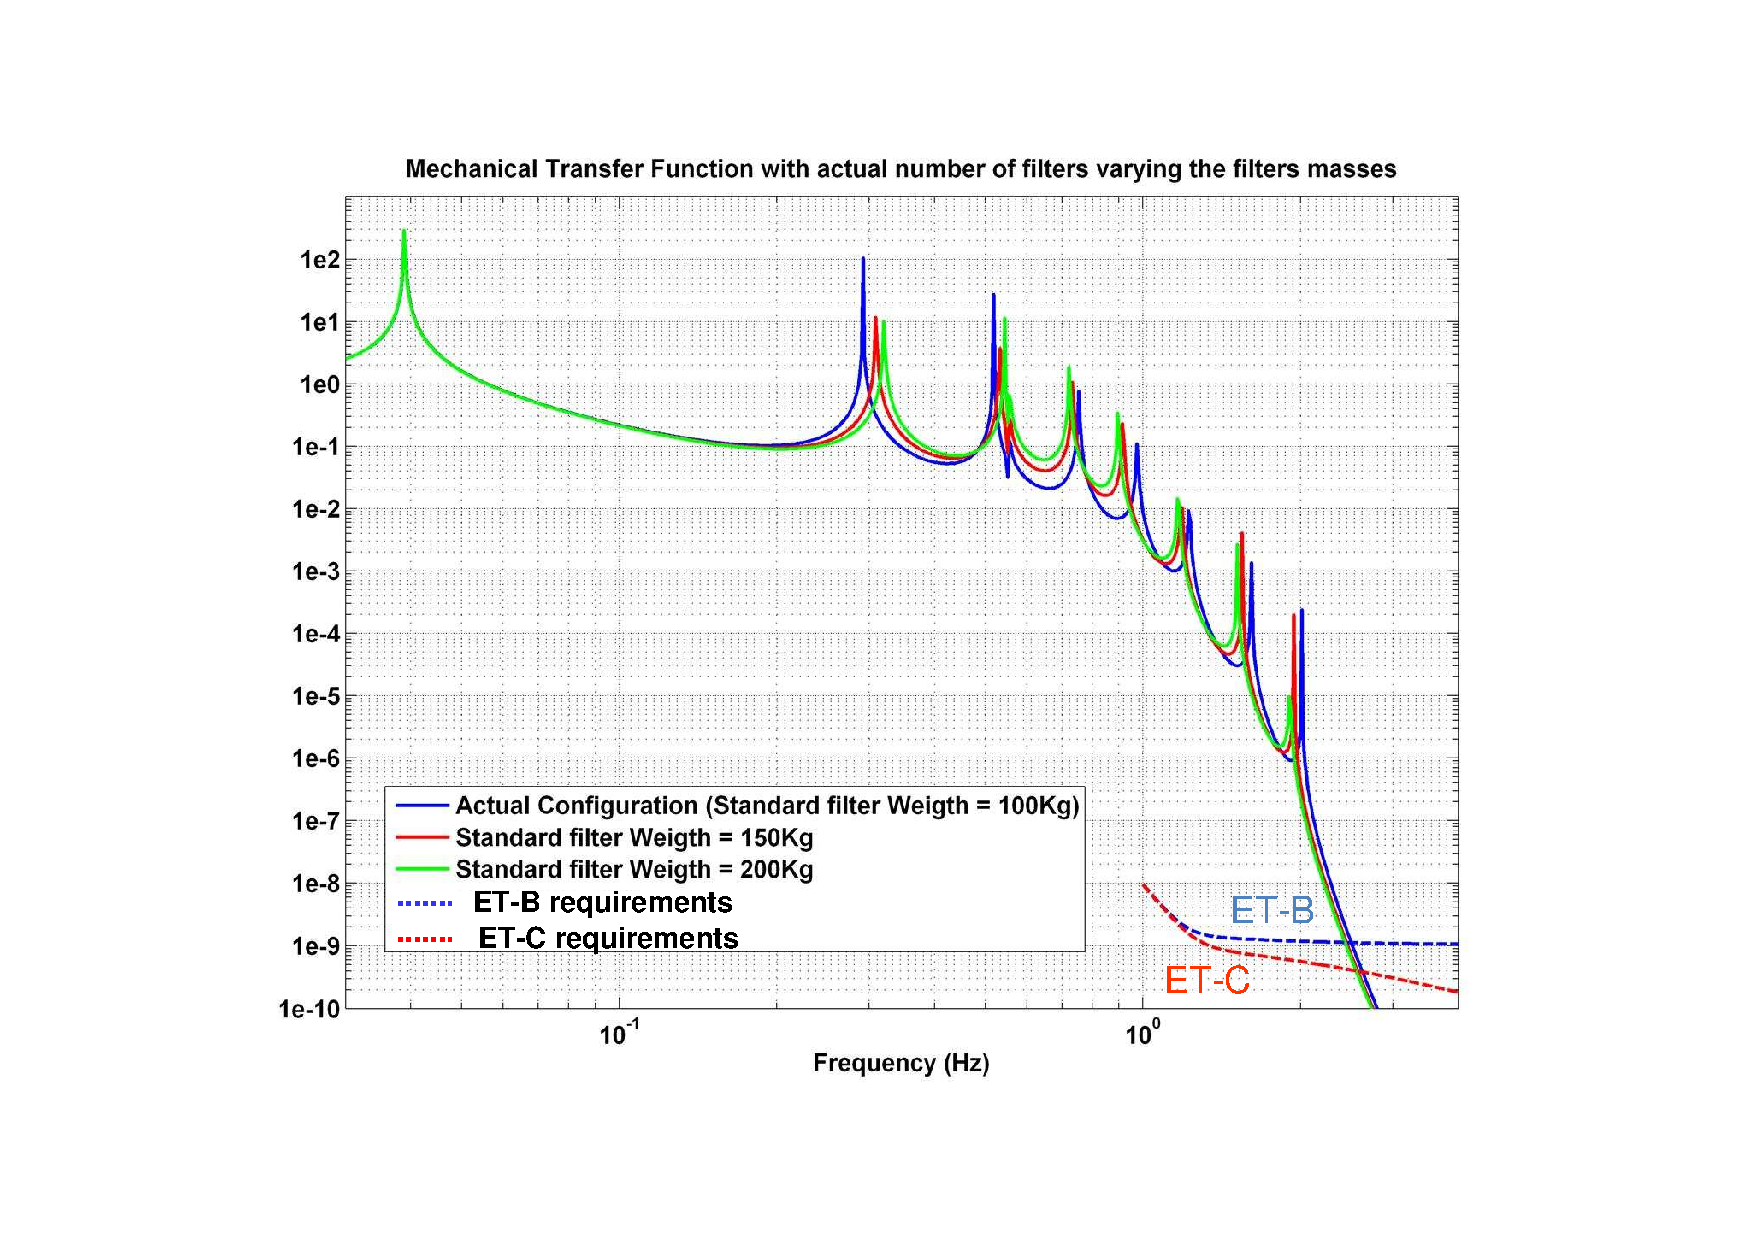
\includegraphics[width=0.9\textwidth]{./Sec_Suspensions/Figures/Par4-Fig2.pdf}
			\caption{The horizontal transfer function of the present \emph{SA} (6 filters weighting 100\,kg each one for a total length of about 9\,m) is compared with the same transfer function changing the mass of each filter (150\,kg and 200\,kg). Also in this case the cross-over frequency with the ET requirements is not remarkably affected by the change of the filter mass.}
\label{Par4Fig2}
	\end{center}
\end{figure}
%
\begin{figure}[t]
	\begin{center}
		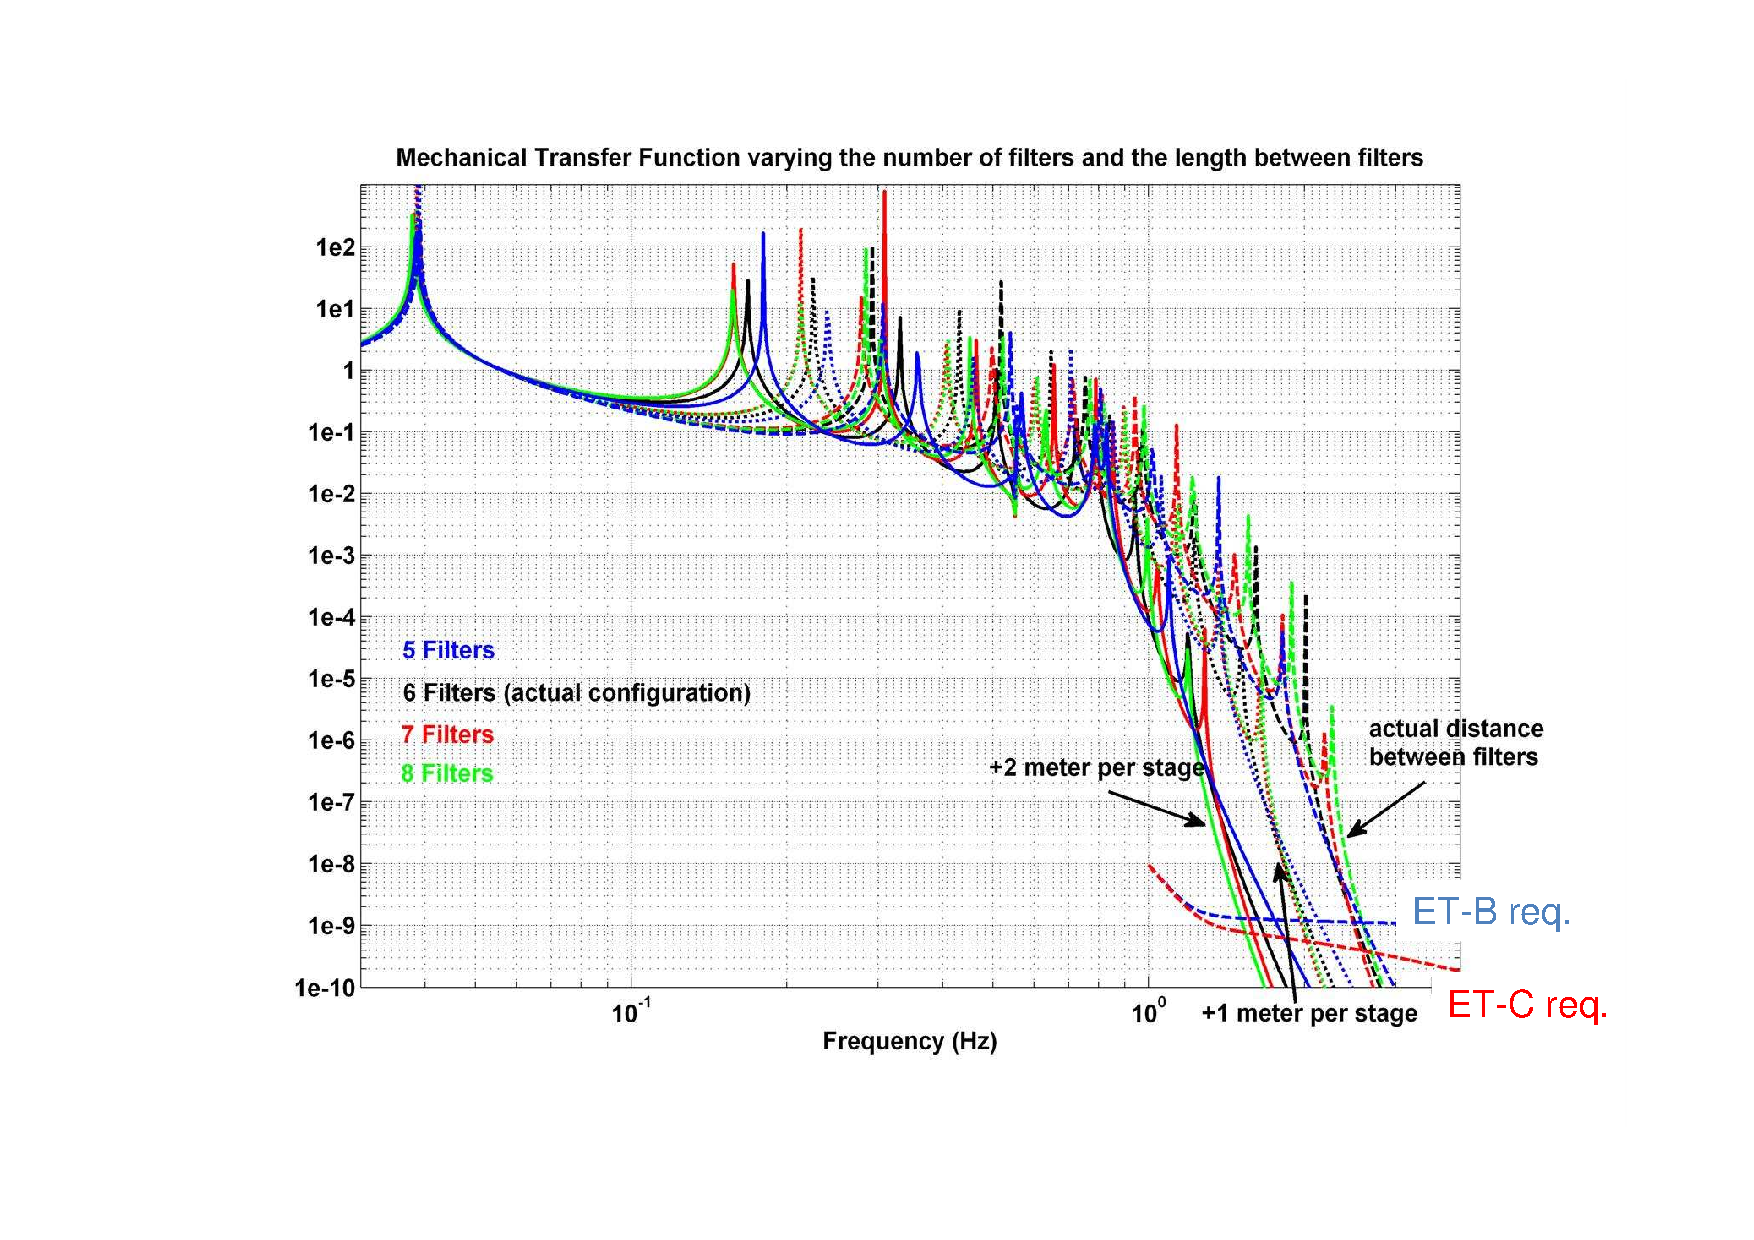
\includegraphics[width=0.9\textwidth]{./Sec_Suspensions/Figures/Par4-Fig3.pdf}
			\caption{Simulation results for different configurations. The horizontal transfer function of the \emph{SA} is plotted changing the number of filters and keeping fixed their relative distances ("equal-spaced" geometry) along the chain (changing, as a consequence, the full length of the SA).}
\label{Par4Fig3}
	\end{center}
\end{figure}
%
The only way to move in the low frequency region the cross-over frequency extending the Einstein Telescope bandwidth below 3 Hz, is to increase the SA chain total length. The simulation results for different configurations can be found in figure~\ref{Par4Fig3} and described in~\cite{Braccini2010March1-3}, while the best solution seems to be represented by a SA with 6 filters and a total length of 17\,m (identical the Virgo configuration, where 5 mechanical filters suspended from an horizontal pre-isolator stage plus the marionette are assembled forming a filter chain about 9\,m long). As shown in Fig.~\ref{Par4Fig4}, with this solution the cross-over frequency has been placed around 1.7--1.8\,Hz, that is considered enough for our purpose. Indeed, Newtonian noise and other technical noise are assumed to prevent an effective detection above a couple of Hz.
%
\begin{figure}[t]
	\begin{center}
		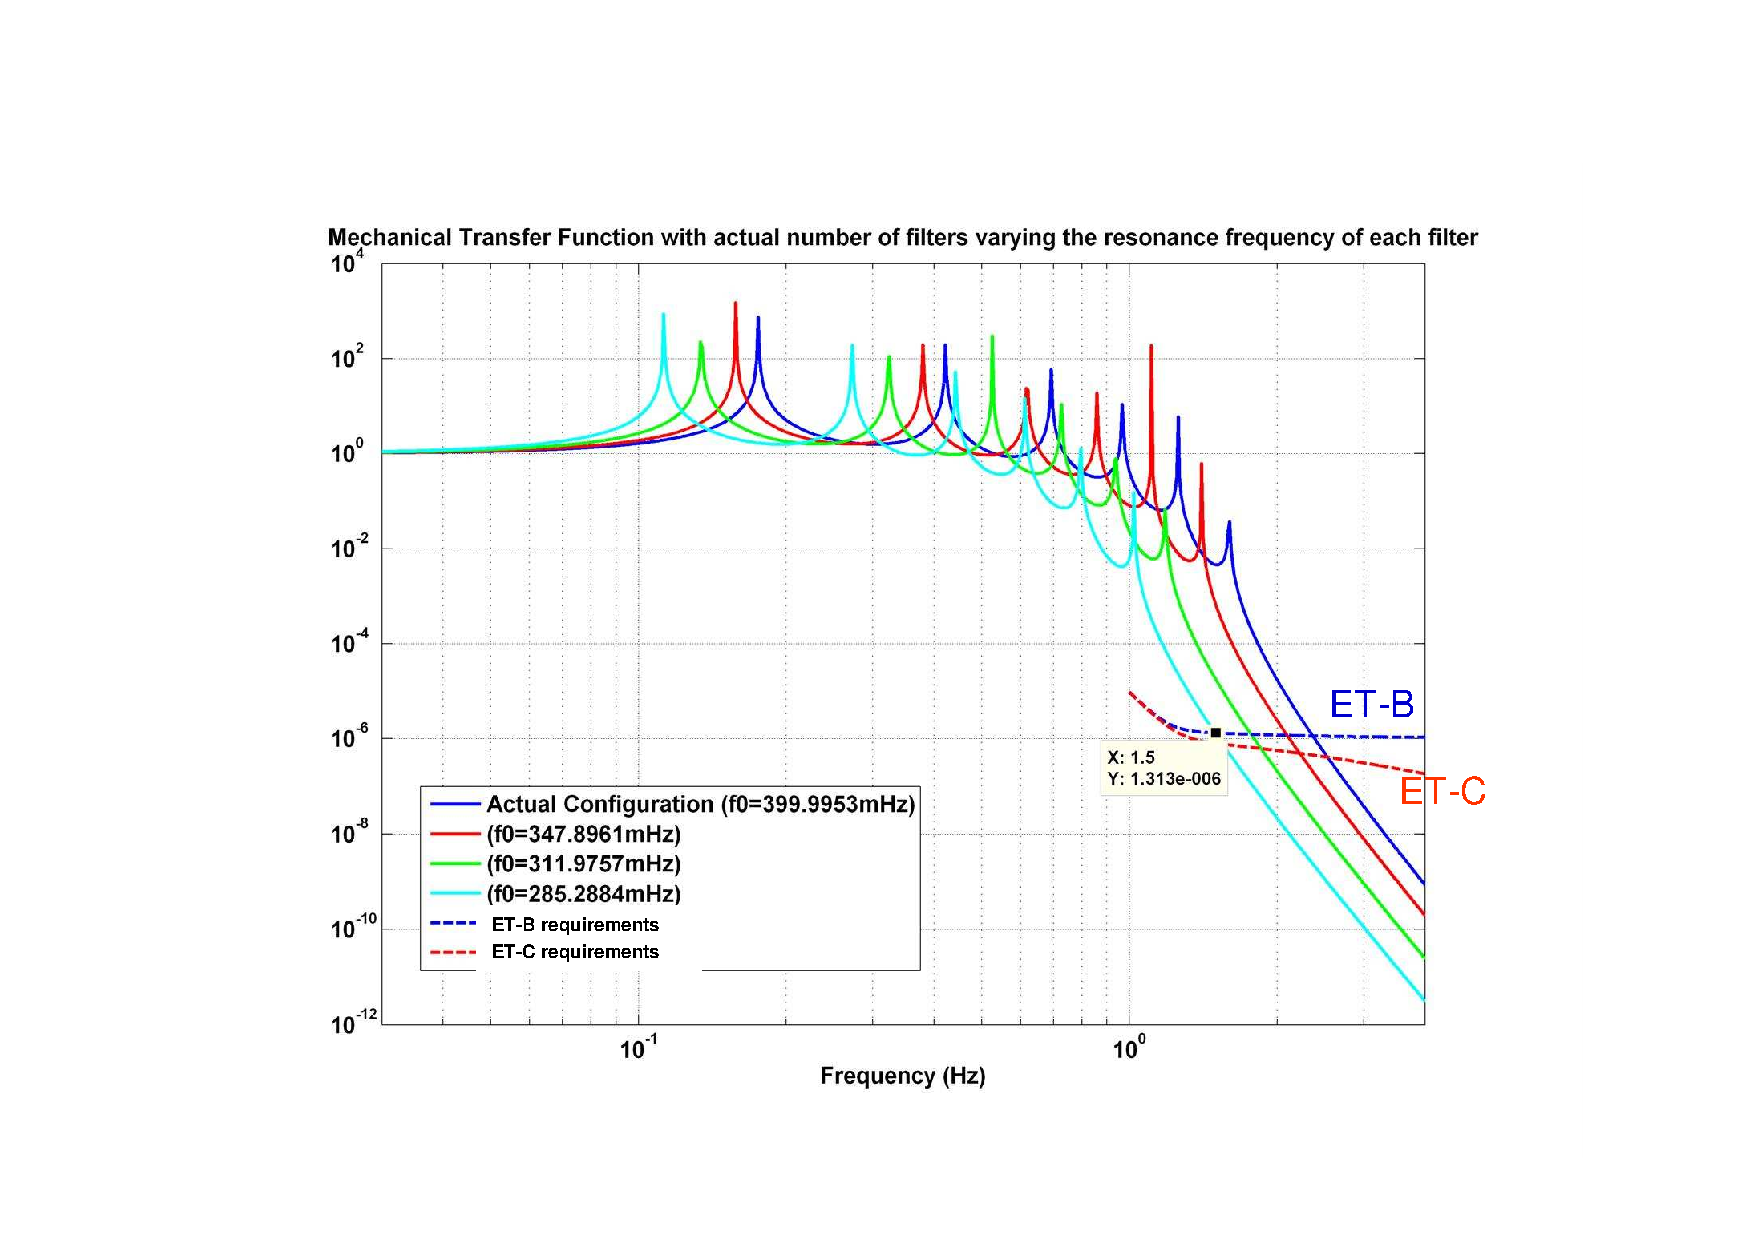
\includegraphics[width=0.9\textwidth]{./Sec_Suspensions/Figures/Par4-Fig5.pdf}
			\caption{Vertical Transfer Function of the SA considering the six stages (as it is now, i.e.\ with the pre-isolator or ``Filter Zero'' plus other five mechanical filters). The different curves have been obtained changing the filter vertical resonant frequency. With filters working around 300\,mHz it is possible to move the cross-over below 2\,Hz.}
\label{Par4Fig5}
	\end{center}
\end{figure}
%
With this configuration, the vertical cut-off frequency of the whole system is set below 1.8\,Hz by tuning each mechanical filter having the main vertical frequency around 300\,mHz (see Fig.~\ref{Par4Fig5}). The corresponding vertical transfer function is plotted in Fig.~\ref{Par4Fig4}. Since the residual seismic noise along the vertical direction, at the level of the mirror, is expected to limit the Einstein Telescope sensitivity again around 1.7--1.8\,Hz, a coupling factor of $10^{-3}$ has been considered. This is due to the fact that the Earth curvature makes plumb lines at a 10\,km distance not parallel each other. At least one mirror has to be inclined with respect to the local plumb line performing the alignment of the cavities. This transmits the residual vertical mirror motion along the beam with the mentioned coupling factor ($10^{-3}$).
%
\begin{figure}[t]
	\begin{center}
		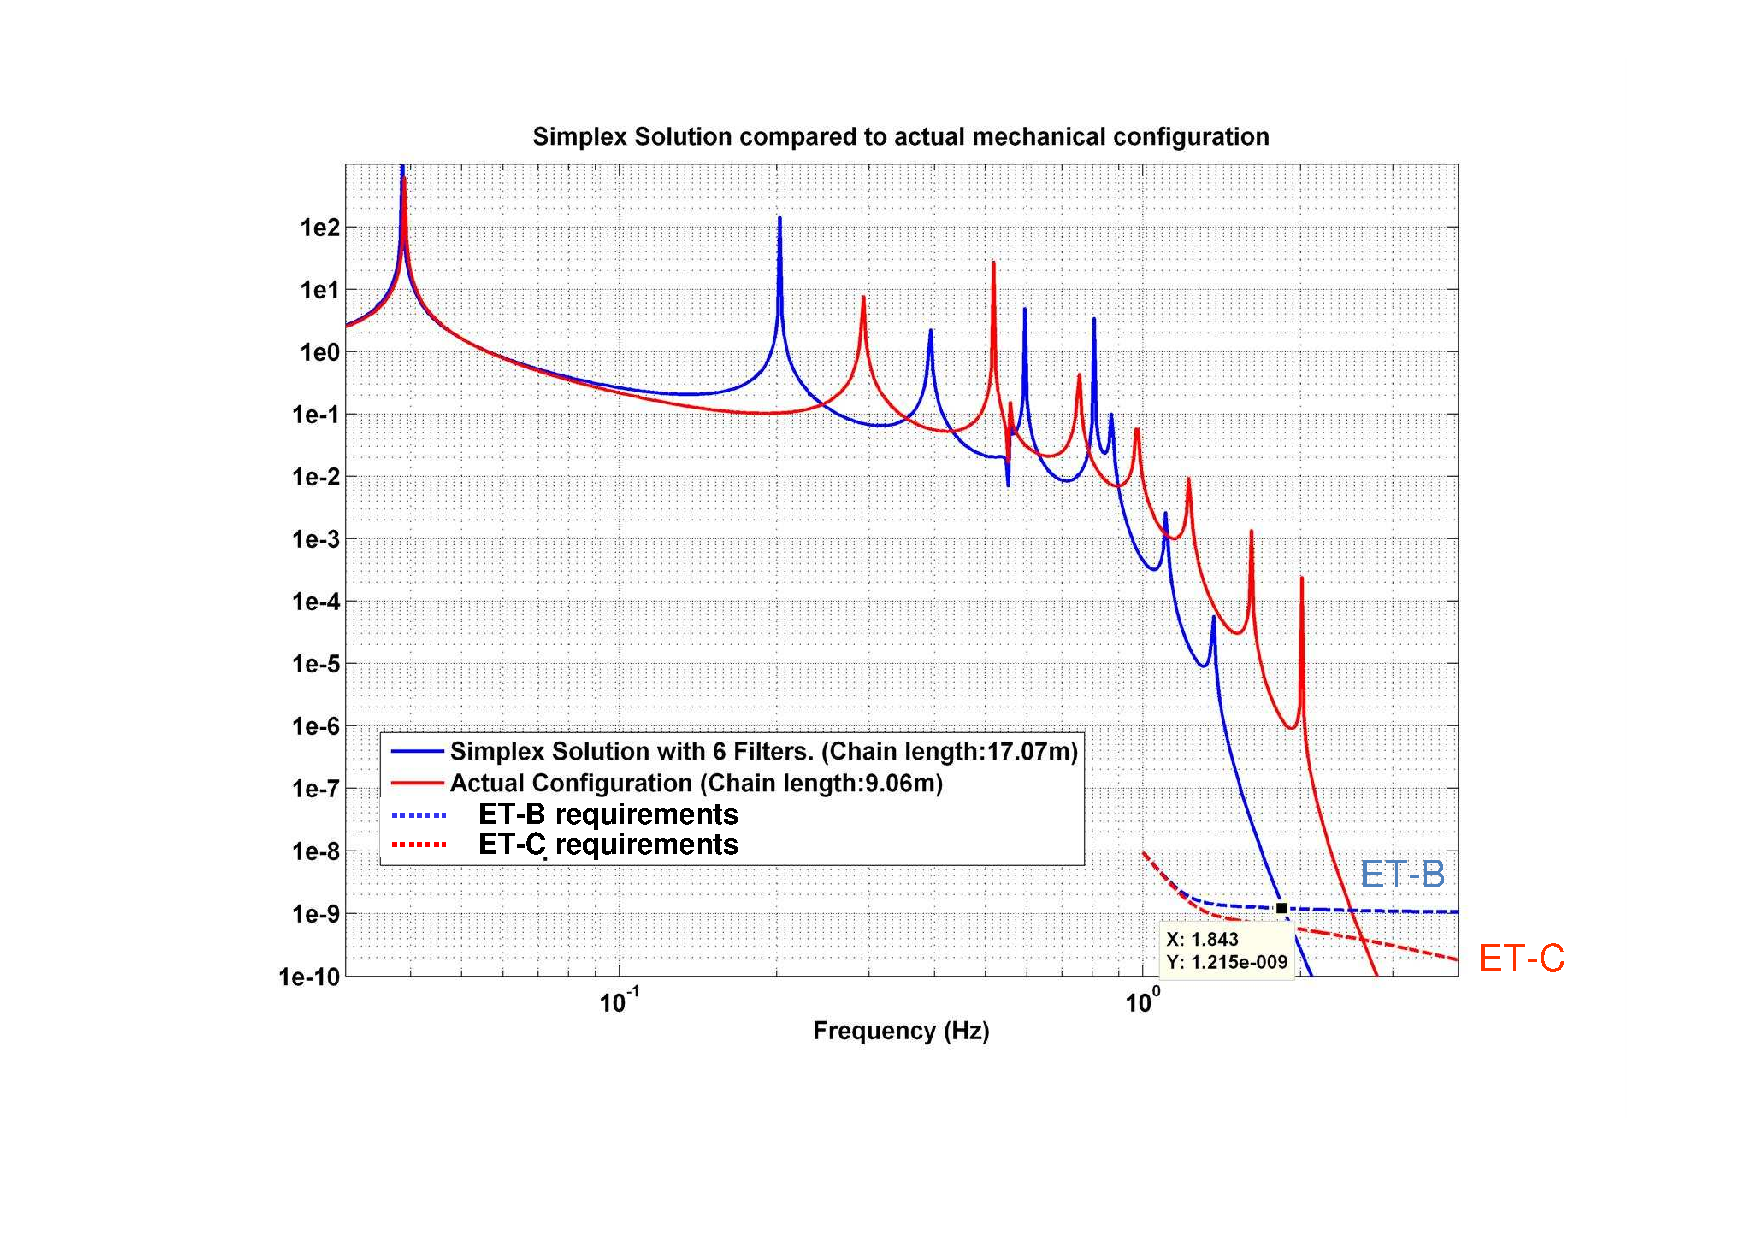
\includegraphics[width=0.9\textwidth]{./Sec_Suspensions/Figures/Par4-Fig4.pdf}
			\caption{The proposed reference solution for the $SA$ configuration of the Einstein Telescope. Other slightly different configurations are discussed in \cite{Braccini2010March1-3}.}
\label{Par4Fig4}
	\end{center}
\end{figure}
%
Since years in Virgo many mechanical filters with a cut-off frequency of around $300$ $mHz$ \emph{Superattenuators} are  in operation  with an excellent stability. By using the Virgo interferometer data, it has been observed that the long-term change of the chain main resonant frequencies induced by the temperature variation under vacuum are 
well inside the line-width of the chain vertical resonances. No effect on the interferometer control is due to this potential disturbance. Moreover, even if the temperature variations induce a motion of the suspension chain and then a slow vertical displacement ({\it {breath}}) of the mirror (a few $mm$ per $^{\circ}C$ is the measured 
value for the Virgo \emph{Superattenuator}), this effect is well within the specifications of any interferometer (vacuum tank provides an excellent temperature stability - fraction of $^{\circ}C$ peak to peak).
The standard SA, presently in operation on the Virgo interferometer, is already well inside the third generation specifications from this point of view too.

In addition, it is important to remind that the requirements in the tens of Hz range are less stringent in Einstein Telescope than in Advanced Virgo (see section 4.1.1.a) and thus, fixing to six (a choice lead by the reduction of the cross-over frequency) the number of filters, a better attenuation performance in the high frequency range is not necessary anymore since the safety margin is large enough in Advanced Virgo and even larger in an underground environment. In conclusion, a SA $17$ $m$ high with 6 magnetic anti-spring filters ("equal-spaced" configuration) tuned with a vertical cut-off frequency around 300 $mHz$, represents the reference solution for the Einstein Telescope. 

In the Appendix \ref{sec:LIGO_filters} we briefly describe the Advanced LIGO  approach to suppress seismic noise. It includes a large two-stages platform  fully active controlled, that, in principle, could improve the compactness of the  ET-LF chain. However a dedicated R\&D study is required for assessing the technical feasibility of this approach in the  ET-LF case.

\paragraph{e) Noise from SA mechanical micro-glitches}

The dislocation motion in the elastic elements of the anti-seismic filter under stress follow a ``self-organized criticality dynamics'' ~\cite{Marchesoni1994}  causing a mechanical noise force along the vertical direction. This force due to micro-glitches exhibits an ``$1/f$-spectrum'', and it is sometime called ``creep noise''. This noise mechanism could affect the interferometer sensitivity. For this reason the Virgo interferometer has been used to set upper limits on the noise floor induced by this spurious mechanism.
\begin{figure}[t]
	\begin{center}
		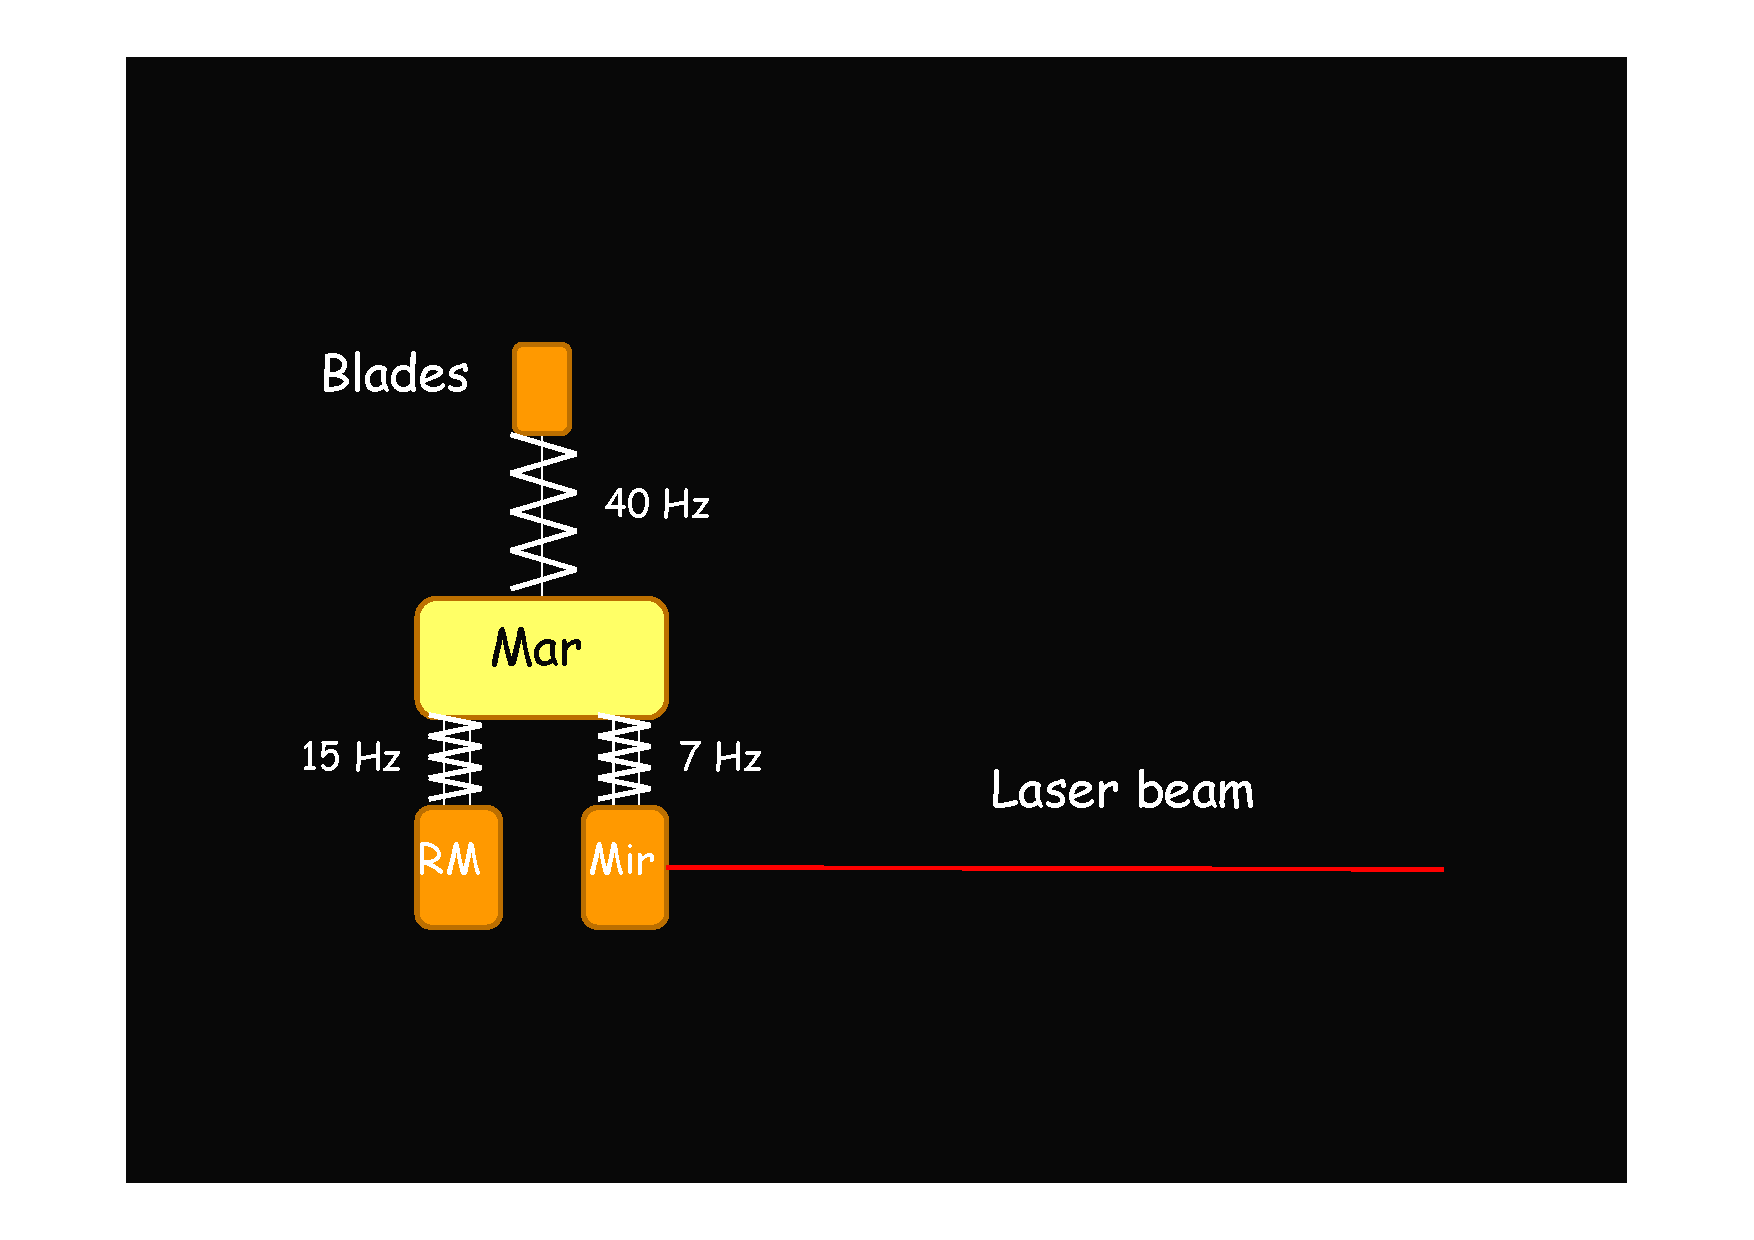
\includegraphics[width=13cm]{./Sec_Suspensions/Figures/Creep-Fig1.pdf}
			\caption{The three vertical modes of the optical payload suspended from the blades of last filter of the chain. For the vertical dynamics the two thin wires in a cradle configuration suspending the reference mass and the mirror can be thought as single vertical springs. As mentioned in the text, the vertical normal modes involve mainly (but not only) displacements of each payload element suspended from the blades: Marionette (\emph{Mar}~-- 40\,Hz), Reference Mass (\emph{RM}~-- 15\,Hz) and Mirror (\emph{Mir}~-- 7\,Hz).}
\label{CFig1}
	\end{center}
\end{figure}
As sketched in Fig.~\ref{CFig1}, the dynamics of the optical payload along the vertical axis can be seen as the motion of three rigid bodies (mirror, reference mass and marionette) connected by three constraints (suspension wires). As a consequence, the payload vertical motion attached to the elastic blade spring of the last filter of the chain exhibits three fundamental modes along the vertical direction involving mainly (but not only) the vertical displacement of the reference mass, mirror and marionette respectively (see Fig.~\ref{CFig1}).
These vertical modes are well visible on the Virgo interferometer output port, namely they appear as peaks on the output photo-diode placed in front of the detector dark fringe (see Fig.~\ref{CFig2}). This means that the modes are excited by some spurious vertical force of unknown origin. 
\begin{figure}[t]
	\begin{center}
		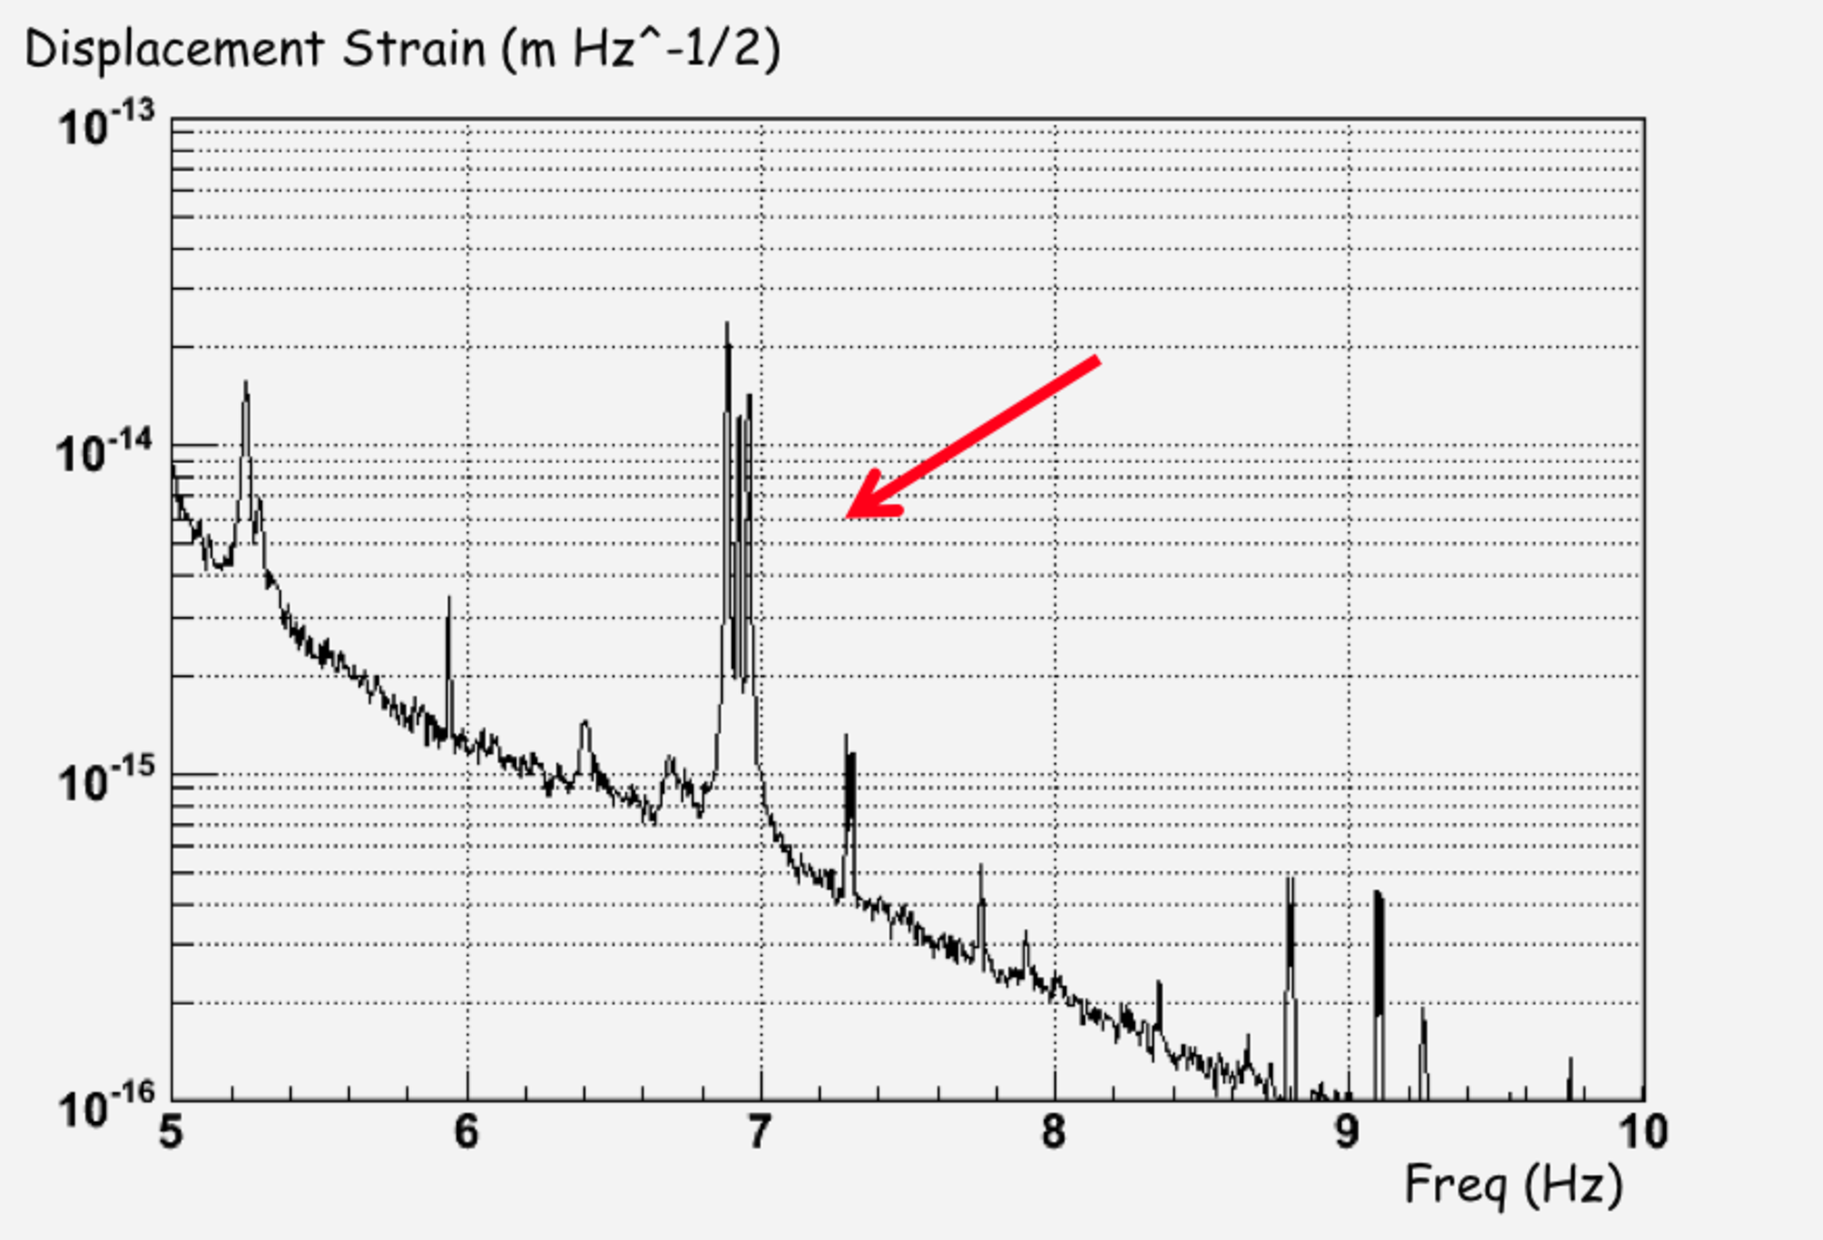
\includegraphics[width=13cm]{./Sec_Suspensions/Figures/Creep-Fig2.pdf}
			\caption{The photo-diode signal at the dark port of the Virgo antenna expressed in strain sensitivity. The four peaks around 7\,Hz correspond to the vertical modes where the mirror displacement is mainly involved. A peak for each one of the four mirrors accommodated along the two Fabry-Perot cavities appears in the dark port (each at a slight different frequency around 7\,Hz).}
\label{CFig2}
	\end{center}
\end{figure}
The micro-creep, such as thermal noise or the electro-mechanical noise floor coming from the coil-magnet actuators are only possible excitation mechanisms. Using the coil-magnet actuators steering the marionette it is possible to excite the three vertical normal modes of the payload. More in general, it is possible to measure the transfer function between the vertical force acting on the marionette and the mirror longitudinal displacement (measured with very high accuracy by the Virgo interferometer). 
\begin{figure}[t]
	\begin{center}
		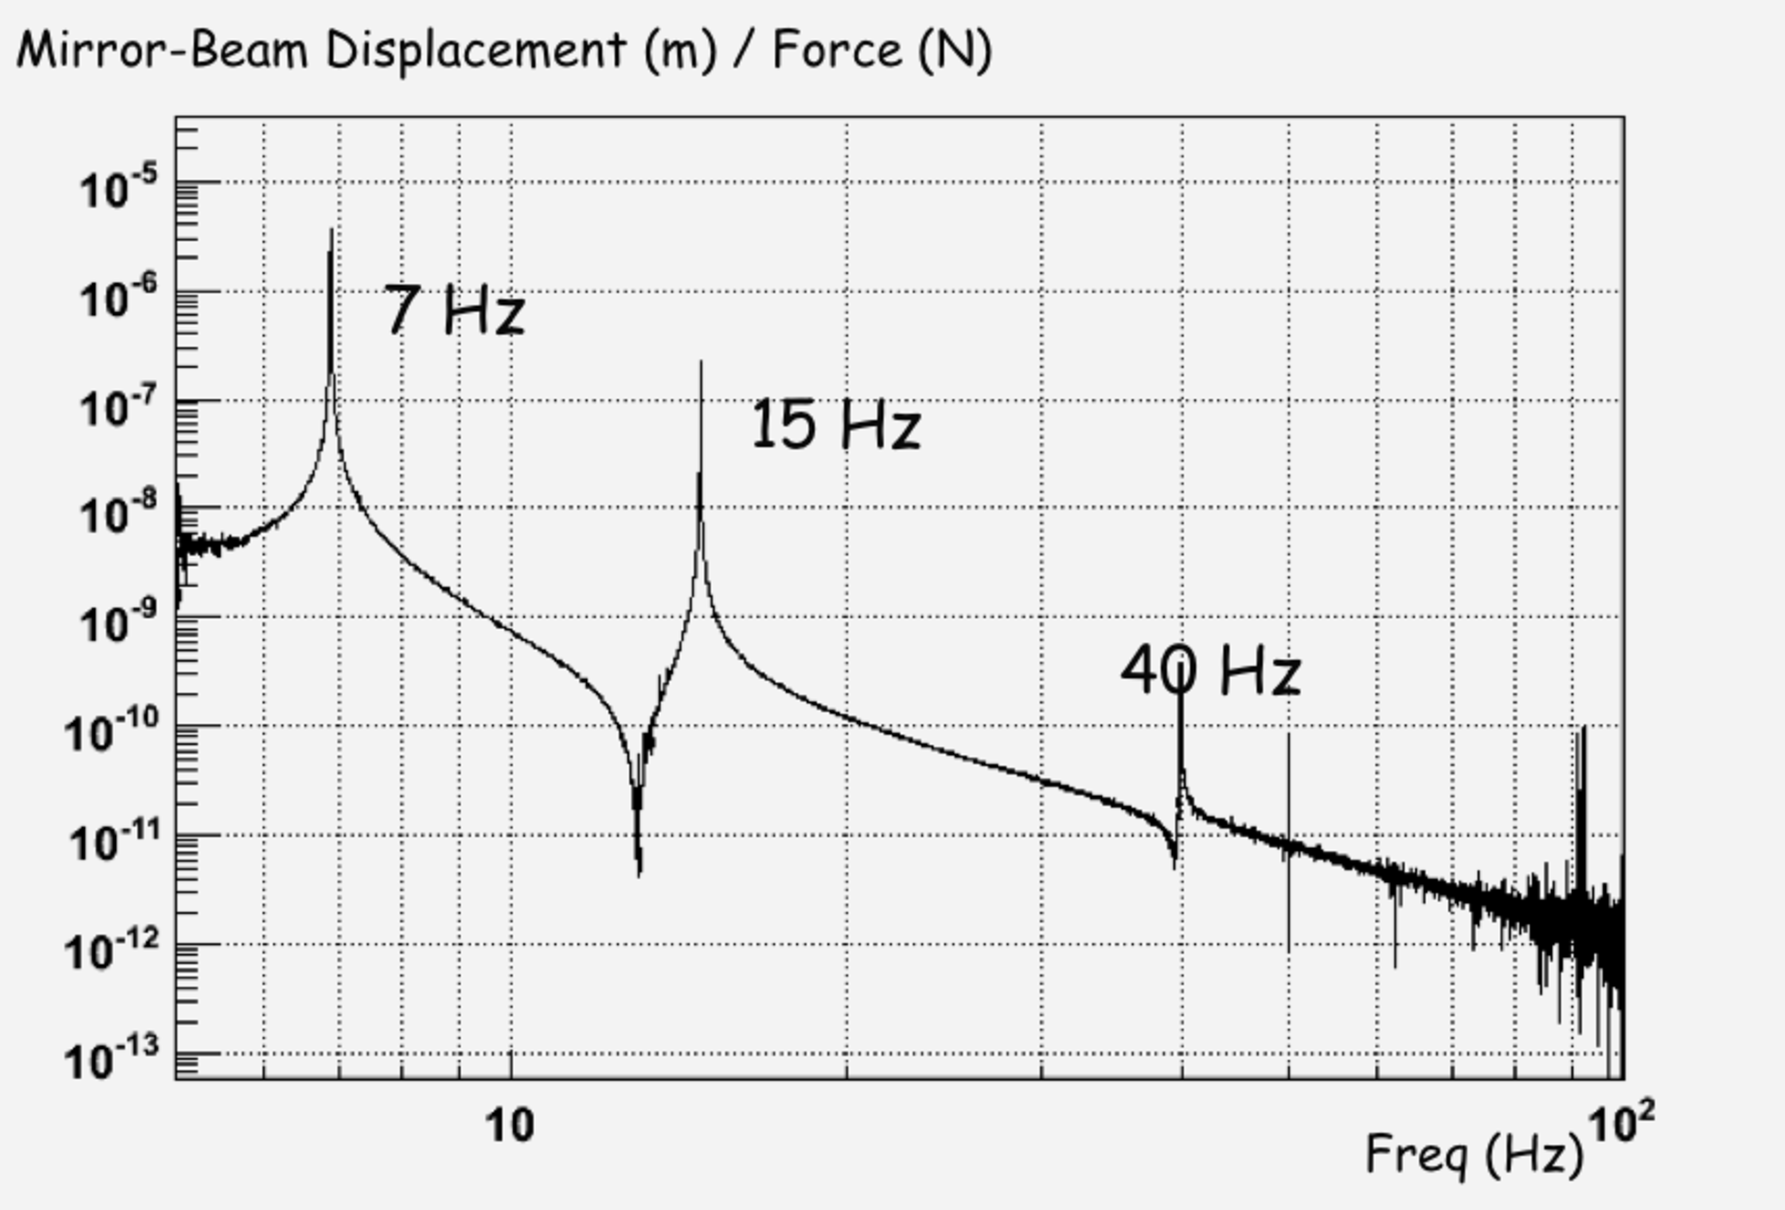
\includegraphics[width=15cm]{./Sec_Suspensions/Figures/Creep-Fig3.pdf}
			\caption{The transfer function between the mirror displacement along the beam (expressed in m) and the vertical force acting on the marionette (expressed in N). The vertical to horizontal coupling-factor (i.e.\ how much the mirror displacement in vertical is transmitted horizontally along the beam) is obviously already included in our measured transfer function and does not require any additional evaluation.}
\label{CFig3}
	\end{center}
\end{figure}
%%
\begin{figure}[t]
	\begin{center}
		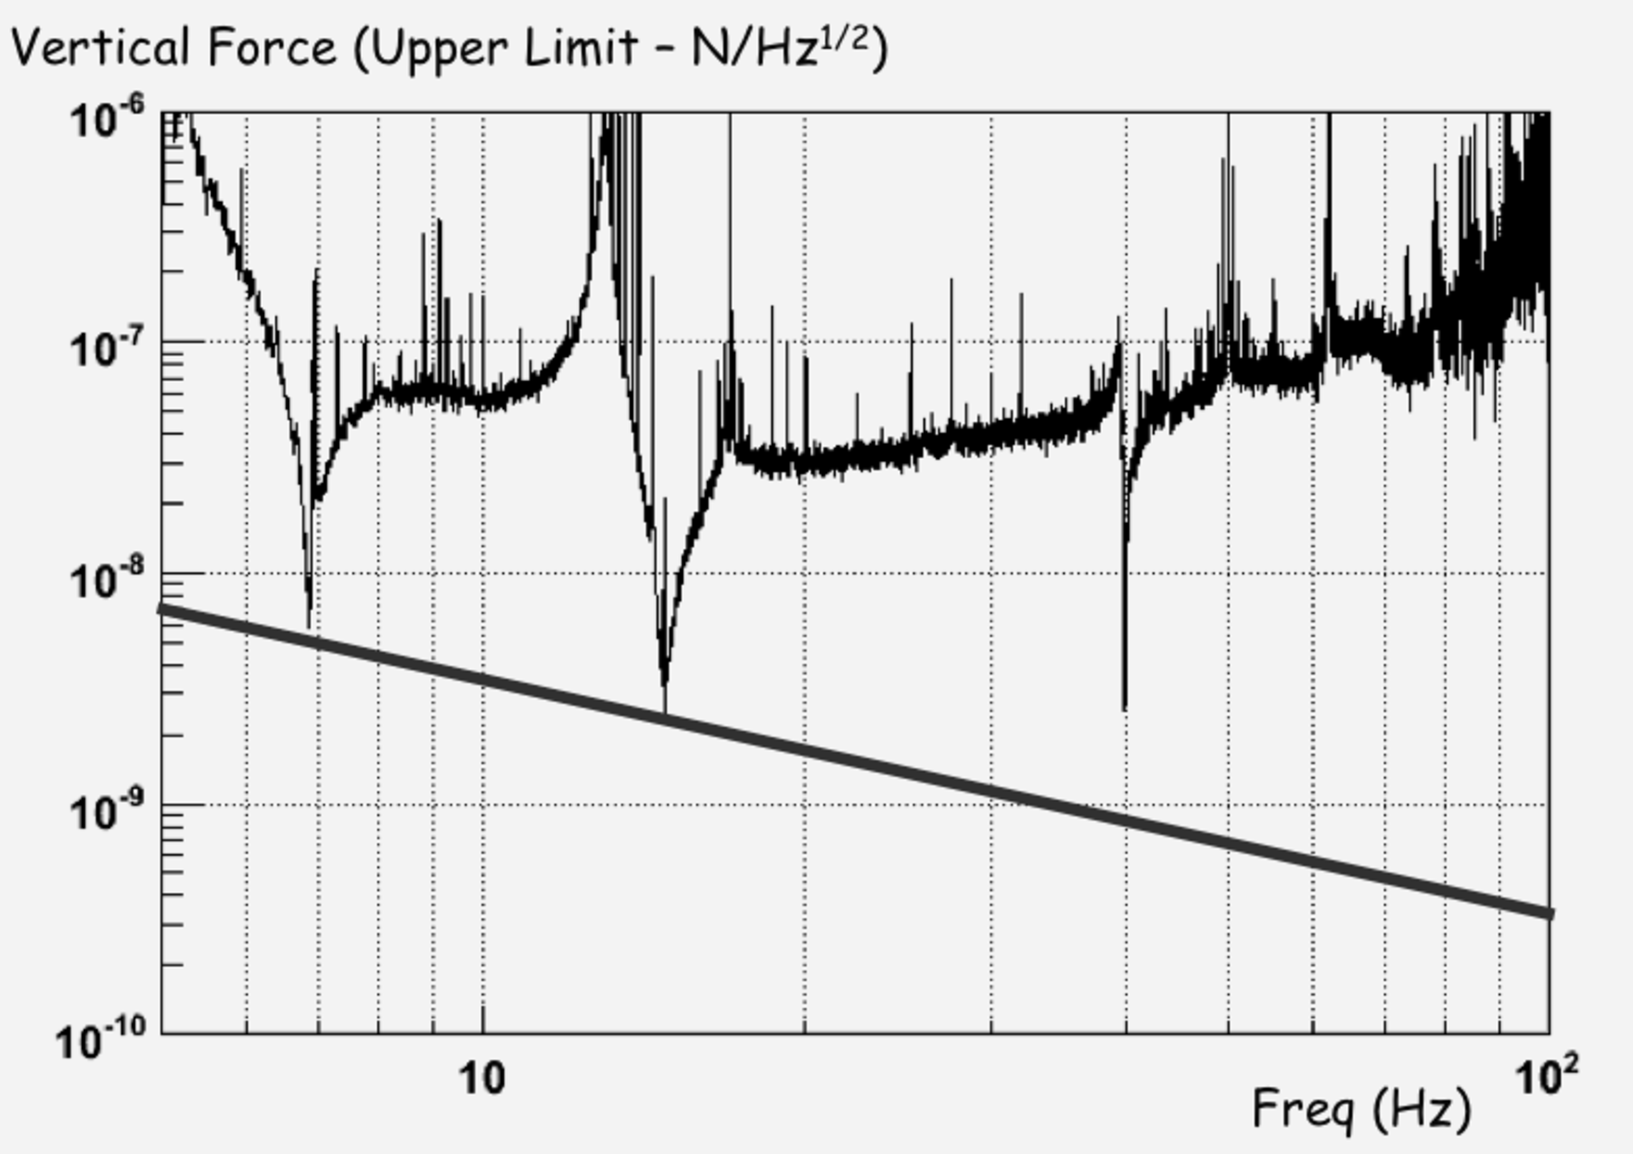
\includegraphics[width=15cm]{./Sec_Suspensions/Figures/Creep-Fig4.pdf}
			\caption{The linear spectral density of the maximum possible vertical force acting on the marionette compatible with the Virgo sensitivity. This is given by the simple procedure described in the text. Since the ``$1/f$-behavior'' of the micro-glitches force is assumed, one can find what is the maximum force having an ``$1/f$-profile'' at the level of the marionette compatible with the Virgo sensitivity. This is given by the minimal ``$1/f$-shape'' line touching the curve that gives the general upper limit on the vertical force just plotted. }
\label{CFig4}
	\end{center}
\end{figure}
%%
\begin{figure}[t]
	\begin{center}
		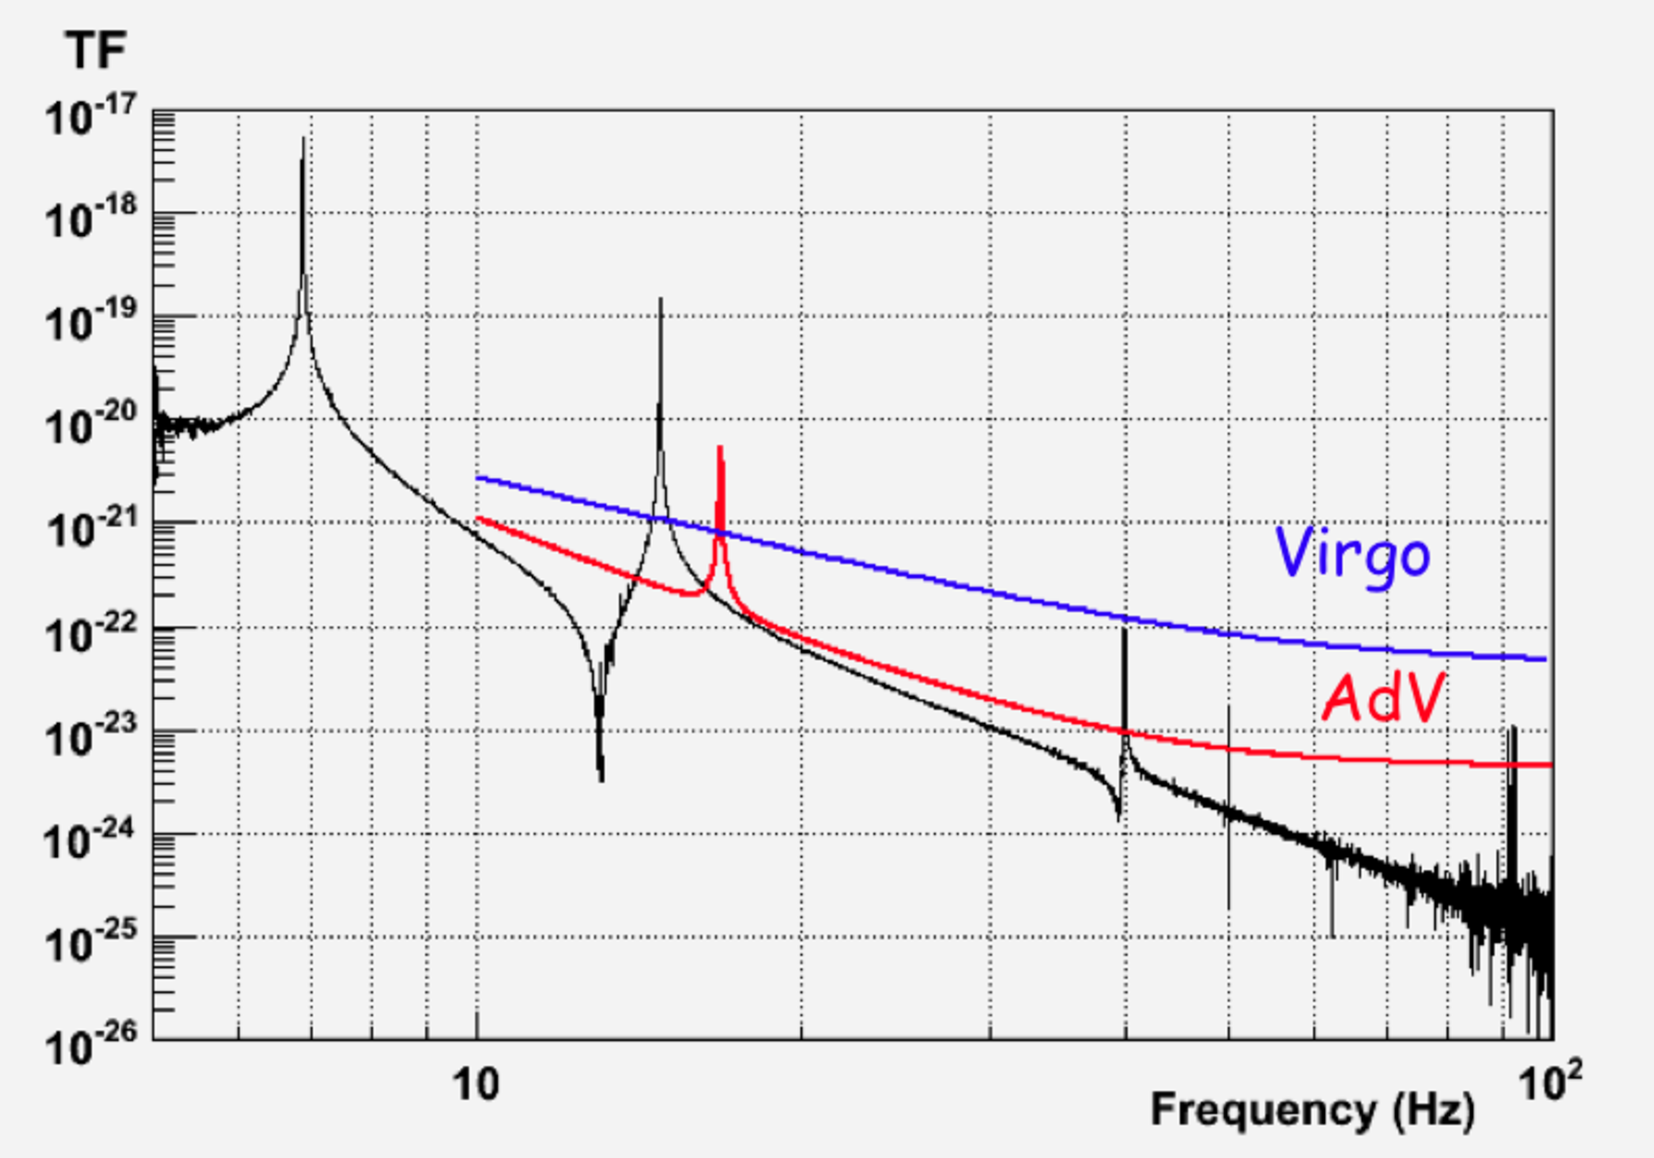
\includegraphics[width=15cm]{./Sec_Suspensions/Figures/Creep-Fig5.pdf}
			\caption{The upper limit of the micro-creep noise floor taking place in vertical on the blades of the last stage is given by the ``$1/f$-force'' upper limit plotted in the previous figure and the mentioned transfer function (stating how this force is transmitted along the beam). The upper limit of this noise floor is compared with the design sensitivity curves of Virgo and AdV. The upper limit, except around the resonant peaks, is enough to state that AdV will not be affected by this source of noise.}
\label{CFig5}
	\end{center}
\end{figure}
%%
The measured transfer function (mirror displacement along the beam, expressed in m over the vertical force applied on the marionette, expressed in N) is plotted in Fig.~\ref{CFig3}. In order to set an upper limit on the vertical force presently acting on the marionette, one can make the ultra-conservative hypothesis (likely not realistic) that the vertical spurious force is dominant in all the band, namely it is responsible of the present sensitivity of the detector. With this assumption, dividing the present sensitivity (expressed in displacement along the beam) by the mentioned transfer function (mirror displacement vs.\ vertical force) the linear spectral density of the maximum vertical force acting on the marionette compatible with the measured sensitivity can be plotted (see Fig.~\ref{CFig4}). 
The deeps due to the three vertical modes of the payload (where the denominator - the transfer function - is large because of the resonant frequencies) are well visible. As mentioned above, the micro-glitches are expected to induce a shot-noise, namely a ``$1/f$-colored force'' thus one can set also the maximum ``$1/f$-like force'' compatible with the present sensitivity (see line at Fig.~\ref{CFig4}). By multiplying the plotted $1/f$-force by the measured transfer function (mirror displacement divided by vertical force on the marionette) one can thus obtain the linear spectral density of the maximum displacement induced by the micro-glitches on the mirror. This upper limit is compared in Fig.~\ref{CFig5} with the sensitivity of the Virgo and AdV. From this figure, one can see that the upper limit just set is sufficient to exclude a dominant contribution in AdV. An important remark is that the micro-glitches are expected to increase when the operation vertical frequency of the anti-seismic filters is reduced. On the other hand, as described in section 4.1.1d, we know that working with seismic filters tuned around 300\,mHz is a must to achieve the required vertical attenuation in the Einstein Telescope. However, several last filters of the \emph{Superattenuator} chains are already working around 300\,mHz and thus our result, excluding a dominant effect due to micro-glitches in Advanced detectors at the level of last filter blades , is valid also at this tuning frequency. The present upper limit is thus surely valid also in Einstein Telescope. On the other hand this upper limit is far (several orders of magnitude) from the third generation sensitivity, especially in the ultra-low frequency range. Since the micro-glitches of the elastic blades taking place on the upper stages of the chain are strongly filtered by the anti-seismic filter underneath, it is obvious that possible problems coming from micro-glitches (if present) can affect the sensitivity of the third generation antenna only if they take place at the level of the last filter(s) of the chain. 
A dedicated R\&D programme to minimize micro-glitch effects on the cryogenic payload (see Appendix) and, if necessary, on the last stage(s) of the \emph{Superattenuator}, is mandatory. In any case this is not expected to affect our anti-seismic isolation strategy, at least on the upper isolation chains.

\paragraph{f) SA control strategy and improvements for ET}

The Suspension Control System plays a crucial role in the interferometer operation. At the top level, it provides DC positioning control and damping of chain normal modes along horizontal, vertical and yaw degrees of freedom. At the bottom it provides the handle to apply residual correction from ground onto the horizontal and yaw degrees of freedom through the steering filter usually left actuation-free. Given the payload suspension point controlled with suitable accuracy, another section of the control is devoted to apply internal forces to the payload and to the interferometer control. The overall structure, described by more than 80 vibrational modes model, is presently (Virgo/Virgo+) controlled by 18 coil-magnet pairs actuators while its status is monitored by using about 20 sensors.

Such controls make use of two main classes of error signals: \emph{local controls} and \emph{global controls}. Local controls use error signals generated by local sensors, accommodated on or close to the suspension structure. Global controls are those whose input signal is generated by sensors located "far" from the suspension mechanics or traced by the interferometer signal. Typical local control sensors are accelerometer located on suspension and position sensors measuring displacement between suspension and suspension enclosure like linear variable differential transformers (\emph{LVDT}). For the payload local control CCD cameras and PSD optical levers are used. Usual global control sensors are photo-diodes or quadrant photo-diodes providing information on suspended optical elements along three directions related to the interferometer beam (longitudinal displacement and two transverse tilts).

In order to ensure drift-less control and to provide suitable response of the system during far earthquakes, with the Virgo set-up, remote sensors and interferometer signals are combined with local sensors. Significant examples are the drift-less local control of mirrors alignment and the Global Inverted-Pendulum Control (\emph{GIPC}). Long suspensions in their \emph{rest} position, without any applied force, are usually up to a several millimetres far from their nominal working point. For this reason the control system has a large dynamics, i.e. it  is able to control over several order of magnitude, and this task is accomplished by using suitable large dynamics sensors and actuators. Once the RMS accuracy of the suspension point (at the top of the mechanical structure) is brought to $\sim 0.1\,\mathrm{\mu m}$, large angular oscillations or DC misalignment can still be present at the level of the payload and local controls are engaged to slow down mirror motion to $\sim 1\,\mathrm{\mu m /s}$ while aligning it from $50\,\mathrm{\mu\text{rad}}$ down to 10\,nrad accuracy. 
In section~\ref{sec:last_stage} some specific issues involving local controls of the payload will be further commented. In fact for ET the role played by the payload and its controls will be crucial in the overall suspension performance even more critically than for Virgo.

In Virgo we successfully tested multi-dynamical range actuators, to apply locking force through the payloads, which are capable of switching between operational modes without introducing discontinuities in the feedback. Meeting injected noise requirements should not be an issue using such devices. To cover the whole huge dynamical range actuation forces are distributed along the chain. In the case of the ET suspension, whatever will be its  final mechanical design,  it seems that we cannot use less than  four actuation points (presently inverted pendulum, steering filter, marionette and mirror). 

Digital controllers used in suspension control system are quite complex: about 250 poles for each suspension requiring about 150 $MFLOPS$ computation capabilities (sustained). One of the key points for a second generation system will be providing tools to ease control engineers life. Today control loops performances are a function of who actually implements the control algorithm. In the past this approach showed to slowly converge to a nearly optimal control. The present evolution of this techniques allows optimal control using almost automated procedures 
much more human independent than $Nyquist$ like approach used so far.
%
\subsubsection{HF interferometer}

As detailed in section 4.1.1.c, the measurements campaign performed with the Virgo interferometer and devoted to evaluate the attenuation performance of the \emph{Superattenuator}, demonstrated that, above 3 Hz, a multistage pendulum suspended to a three legs mechanical structure, as pre-isolator stage, is compliant with the ET requirements. The results reported in figure~\ref{FigSusp5} have been obtained by using a \emph{Superattenuator} 
with \emph{six} seismic filters (for a total length of about 9\,m) hung to a platform accommodated on top of the Inverted Pendulum which has been by-passed during the suspension point excitation phase of the measurements. This represents a good safety margin from attenuation point of view, because passing the seismic noise through the mechanical structure of the Inverted Pendulum, it will be additionally attenuated by a factor around 20--40\,dB.

Starting from the long experience acquired in operating a similar mechanical system for seismic noise suppression, a base line for the LF and HF Detectors of the ET Project has been tracked. It is based a seismic attenuation system designed for the Virgo interferometer with common peculiarities: the first one can be conceived extending the detection bandwidth below 3 Hz by improving the chain total length up to 17\,m , while for the second a Virgo-like \emph{Superattenuator} can be built. The advantages of this choice are different:  
\begin{itemize}
\item even considering a conservative cut-off frequency of the whole system around 5\,Hz, it turns out that there will be a wide overlap between the HF Interferometer bandwidth the LF Interferometer one (following our indication starting around 2\,Hz);
\item the construction technology, mainly based on the use of magnetic anti-spring, has been deeply tested in vacuum for a very long time period (about ten years);
\item the behavior of high stressed elastic elements (blades and wires) has been 
studied;
\item many mechanical and electro-mechanical elements are compatible with cryogenic environment (see the Appendix \ref{sec:cryo_filters});
\item the upgrades, presently in progress for the Virgo \emph{Superattenuator}, 
can be used for this application too.
\end{itemize}

In this context and considering the ET requirements the choice of the Virgo \emph{Superattenuator} as seismic isolation system for the third generation of gravitational wave detector,seems to be the natural one.

\FloatBarrier 

\longetbox{r}{box:Final}{Final considerations on Suspension for ET-LF and ET-HF}
{ 
\begin{itemize}
\item Above 3 Hz the present Virgo \emph{Superattenuator} is compliant with the ET requirements. Minor changes are needed to extend the detection bandwidth in the low frequency region (below 3Hz). The \emph{Superattenuator} is a very good candidate to be installed in the \emph {LF Interferometer} for the following reasons:
	\begin{itemize}
	\item it has well tested behavior over 10 years activity;
	\item it has well tested technology;
	\item vacuum compatibility of crucial elements (under vacuum for many years);
	\item many mechanical and electro-mechanical elements compatible with cryogenic environment.
	\end{itemize}
\item A \emph{Superattenuator} 17 m tall with six stages (filters) in "equal-spaced" configuration and filter tuning (using the magnetic anti-spring) with a vertical cut-off around 300 mHz represents the reference solution for the ET Project. With this set-up a suspension system with a conservative cross-over frequency around 1.8 Hz (compliant with ET requirements) can be built.
\item The Virgo \emph{Superattenuator} could be used as seismic isolation system of the \emph {HF Interferometer} for the following reasons:
	\begin{itemize}
		\item the attenuation performance is compliant with the ET requirements;
		\item the cross-over frequency (around 5 Hz) is good for this purpose;
		\item the technology used (magnetic anti-spring filters) for its construction is well tested ;
		\item all the upgrades of the system, presently in progress, are available also for this application.
	\end{itemize}
\item Ten years of activity on the control system of the \emph{Superattenuator} represents a clear demonstration that a feed-back control at low-noise can be used to improve its performance in the low frequency region (below 5 Hz). The acquired experience on this subject is a valuable starting point for the commissioning of next generation detectors.
\item The construction of the seismic isolation systems for Einstein Telescope could start immediately after a slight refinement of the project. Thanks to the Virgo experience the \emph{Superattenuator}, developed to filter seismic noise at the mirror level, is the reference solution for the project.
\end{itemize}
}
%%%
\subsubsection{Upper-lower suspension interface}
\label{Upper_lower_suspension_interface}

As described all along this document, the ET Project is based on two different detectors. The first one aimed to the detection of gravitational wave signals in the low frequency range (\emph{LF Interferometer}) and the second one for the detection of high frequency signals (\emph{HF Interferometer}). The LF experimental apparatus will have a detection bandwidth as wide as possible in this specific region adopting, as seismic isolation system, the Virgo \emph{Superattenuator}. The main difference is represented by the length of the multistage pendulum (for details see section 4.1.1.d), an important parameter to move the cut-off frequency of the whole system to the best value in accordance with the ET requirements (around 2 Hz for a total chain length of about 17\,m).
The main characteristic of the LF Detector is that the suspension upper part will be at room temperature while the payload is maintained at cryogenic temperature for beating the thermal noise limit. These working conditions will not be present in the HF Detector where a seismic isolation system based on the Virgo \emph{Superattenuator} 9\,m high will be operated at room temperature thanks to its attenuation performance above 3\,Hz compliant with the ET requirements. 

For this project a complex vacuum system has been studied with both interferometers within the same tunnel and in particular with the pipes for LF Interferometer running on top of those ones of the HF Detector. This configuration will include a cooling shield containing the payload within the vacuum tower basement of the LF Interferometer. While the test mass and the penultimate stage of the suspension will be accommodated within the cryostat, a suspension wire made of Ti-6Al-4V will be used to suspend the payload from the \emph{Superattenuator} upper part at room temperature (see section 3.4). This interconnection element has a key role in preserving the thermal isolation between the payload and the suspension upper part. Moreover, the cryostat structure will have a hole through which this suspension wire will pass. This hole should be large enough to avoid possible wire friction during standard working condition, but it should not create an important and undesirable thermal input for the cryostat operation. The penultimate stage, indeed, will be directly connected through a thermal link to an ancillary suspension where a \emph{cold box} will be installed. In this way the heat extraction from the mirror is obtained via the suspension fibres attached to the penultimate stage, and then through the thermal link toward the ancillary suspension.

Since the hole in the cryostat structure will be also used for pure helium gas exchange during the cooling down process (pure helium gas will be injected within the experimental volume to speed up the cooling down/warming up procedure), it will be equipped with a mechanical shutter (vacuum tight) driven by a stepping motor (remotely controlled for opening/closing procedure) to be installed in the roof structure separating the tower upper part from the bottom one. This mechanical solution together with an adequate pumping system and a well defined evacuation procedure will be important steps to reach the needed vacuum level. 


\FloatBarrier
\subsection{Mirror last stage suspension}
\label{sec:last_stage}

%\emph{Author: F.\ Ricci}

The Last Stage Suspension (LSS) is the system designed to couple the test mass to the \emph{Superattenuator} chain, to compensate the residual seismic noise and to steer the mirror through internal forces exerted from the last Superattenuator element (\ref{steeringF})~\cite{LSSpaper1999}.

The main components of a Virgo-like LSS are the Marionette, the Recoil Mass (RM)  and the Mirror as shown in figure~\ref{LSSfig}.
The marionette  ($\rm M_1$) is the first stage used to control the mirror position with coil-magnet actuators operating between the upper suspension stage
and marionette arms; the recoil mass ($\rm M_3$)  is used for the Mirror ($\rm M_2$) steering and its protection, it carries the coils of the e.m.\ actuators acting on the mirror rear side.



Using the last stage we have to perform the alignment  of the test masses and compensate the residual seismic noise below 1\,Hz.
LSS includes  a dedicated  set up for controlling  the position and orientation of the suspended masses to the respect of the local reference frame It is useful   also  for dumping  large oscillation eventually excited during the adjustment phase. 

\noindent
The last stage has to operate in  an ultra high vacuum environment. Moreover, to avoid extra dumping mechanisms and spurious couplings  the use of magnetic and electrostatic materials must be limited as much as possible. In particular the choice of the suspension material and its shape   is crucial for limiting  the thermal noise contribution of the interferometer sensitivity.

\begin{figure}[t!]
	\begin{center}
		 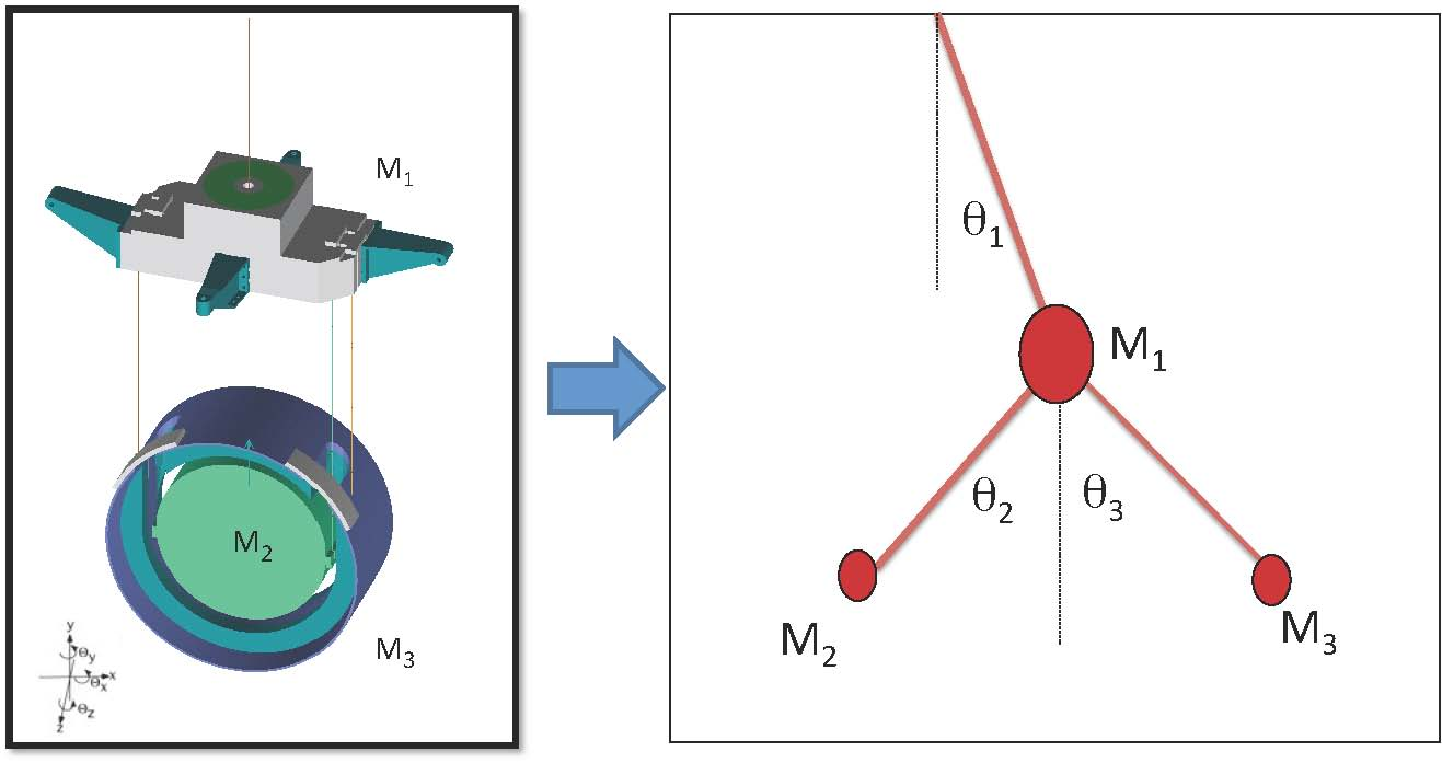
\includegraphics[width=14cm]{Sec_Suspensions/Figures/LSS_branched.pdf}
			\caption{Left: Sketch of the Virgo-like Last Stage suspension. Right: Scheme using the point-like masses $\rm M_1$: Marionette, $\rm M_2$: Mirror, $\rm M_3: Recoil Mass$}		
			\label{LSSfig}
	\end{center}
\end{figure}

The mechanical and electromagnetic design is conceived following specific requirements:
\begin{itemize}
\item{The mechanical resonance frequencies of the last stage elements must be as high as possible to avoid spurious thermal noise contributions to the interferometer output}
\item{The steering of the optical elements needs to be performed in an ultra-high vacuum (UHV) space.}
\item{The payload components (marionette, reaction mass and e.m.\ actuators) has to be conceived in such a way to limit the dust contamination of the optical element during the assembly phase and in operation (class 1 clean-room compatibility)}
\item{It is necessary to limit the cross-talk effects among the various degrees of freedom to be controlled. This implies an accurate design of the electromagnetic actuators and a careful design of the suspension point of the mechanical elements. }
\end{itemize}

In particular, to fulfill the last requirement to simplify the  Multi Input Multi Output (MIMO)  control,  we have to keep

\begin{itemize}
\item{the center of masses alined along the Superattenuator axis}
\item{ the three principal axis of the ellipsoid of inertia of each suspended body parallel to the gravity line, the interferometer optical axis and its transversal direction.}
\end{itemize}

Finally, we add a couple of constraints derived from our past experience of  controlling the Virgo mirrors: 
\begin{itemize}
\item{we need to limit   the recoil effect  by optimising  the mass values of the suspended elements,}  
\item{we should   avoid   the insert  of  composite bodies ( as for example a mirror clamped to an external frame ) along the main beam path, which can cause the presence of spurious resonance in the control bandwidth of he instrument.}
\end{itemize}
In the next sections,  we model the thermal noise of the mirror suspension and  we describe the mechanical designs  for LF- and HF-ET.  Then we focus on the control issues and the related actuators and sensors. Finally we discuss the technologies to be developed.

\FloatBarrier
\subsubsection{Material selection for the last stage suspension}
\label{sec:mat_lss}

%\emph{Author(s): R.\ Nawrodt}

The last stage suspension is the most critical point of the whole suspension chain. It determines the thermal noise of the suspension elements. Thus, low mechanical loss materials in combination with a monolithic suspension technique as used in GEO600~\cite{Plissi1998,Willke2002} and the Advanced Detectors~\cite{aLIGO,Robertson2002,Cumming2009} is preferred. Here the material of choice is fused silica which fulfills these requirements and has been studies in great detail in the past. 

In the low temperature detector the suspension elements have to fulfill a second crucial duty - they have to extract the thermal load that is put into the optical component by the laser beam. This additionally demand rules out fused silica as a suspension element due to its very small thermal conductivity at low temperatures as an amorphous material (see figure~\ref{fig:bulk_TC}). In contrast, crystalline materials have a very high thermal conductivity at low temperatures. 

\begin{figure}[!h]
\begin{center}
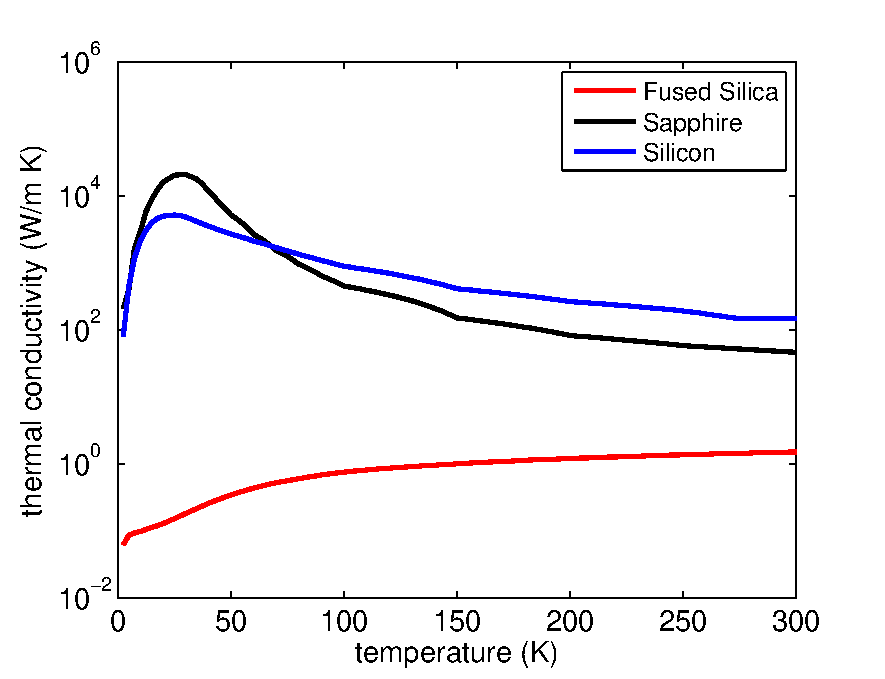
\includegraphics[scale=0.7]{./Sec_Suspensions/Figures/bulk_TC.pdf}
\end{center}
\caption{Thermal conductivity of bulk fused silica, sapphire and silicon. The plotted values are obtained from Touloukian~\cite{Touloukian1970_kappa_metal,Touloukian1970_kappa_nonmetal} as `recommended' curves.}
\label{fig:bulk_TC}
\end{figure}

Both materials---silicon and sapphire---show a large thermal conductivity in the temperature region of interest (typically below 20\,K which will be shown later by means of thermal noise considerations in section~\ref{sec:LF_mirror_def}). Sapphire has a higher thermal conductivity as silicon below 20\,K. Sapphire fibres for heat extraction have been investigated in detail by Japanese groups for CLIO and LCGT~\cite{Uchiyama2000,Tomaru2002b,Suzuki2003}.

A third point for the selection of the suspension material is the possibility to bond the suspension element to the test mass. As will be shown later the most likely substrate material will be silicon for the Einstein Telescope due to its availability in large pieces. Sapphire samples are not available in large enough pieces which are needed for the LF detector (see section~\ref{sec:material}). The bond strength of sapphire-silicon~\cite{Dari2010} bonds is smaller than silicon-silicon~\cite{Veggel2009,Dari2010} bonds based on hydroxid-catalysis-bonding. The reason for the weaker bonds in a sapphire-silicon configuration is so far unknown---beside direct chemical effects during the bonding process imperfections in the polished surfaces of the bonded samples are very likely to be the origin of this effect. Besides the weaker bonds the different coefficients of thermal expansion might cause stress during operation at low temperatures which might reduce the reliability of the sapphire-silicon bonds.

All these considerations lead to a preferred design based solely on silicon. Silicon suspension elements are currently under investigation in the form of fibres~\cite{articolofibresil} and ribbon-like structures~\cite{Reid2006}. Details about the ongoing work can be found in section~\ref{sec:technologies}.

The thermal conductivity of crystalline materials is dependent on different effect:

\begin{itemize}
\item the concentration of impurities,
\item the sample dimension,
\item the phonon density at the given temperature.
\end{itemize}

These properties define the shape of the thermal conductivity curve in dependence on temperature. At higher temperatures thermal phonons collide with other phonons or impurities which leads to a finite thermal conductivity. At lower temperatures the effect of phonon-phonon collision becomes weaker due to the reduced density of phonons. The impurities dominate this region. At sufficient low impurity concentrations the thermal phonons begin to collide with the sample boundaries before other collisions. The phonons propagate now ballistically and the thermal conductivity becomes geometry dependent. At even lower temperatures the thermal conductivity decreases due to a lack of available phonons for carrying heat. This general behaviour of a crystalline material can be seen from figure~\ref{fig:bulk_TC}. 

A very high impurity density is present in polycrystalline samples. Here, the grain boundary act as very efficient scattering surfaceimpurity and reduce the thermal conductivity of the sample (see figure~\ref{fig:Si_isotope}). In order to get high thermal conductivity suspension elements polycrystalline samples need to be avoided.

The effect of impurities and phonon-phonon scattering by means of N- and U-processes on thermal conductivity has been studied in detail in the past~\cite{Callaway1959, Callaway1960}. For very pure silicon samples it was observed that the natural composition of isotopes acts as scattering centers as well. If these scattering centers are removed by enriching the silicon with one isotope the thermal conductivity can be even further increased (see figure~\ref{fig:Si_isotope}). 

\begin{figure}[!h]
\begin{center}
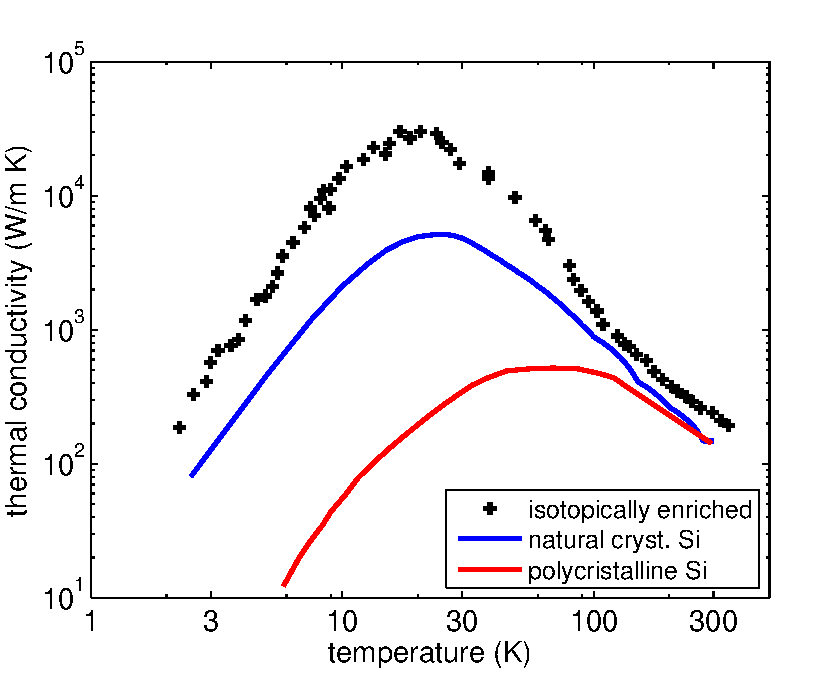
\includegraphics[scale=0.7]{./Sec_Suspensions/Figures/Si_TC_isotope.pdf}
\end{center}
\caption{Thermal conductivity of silicon. The results for natural and the polycrystalline silicon are obtained from \cite{Touloukian1970_kappa_metal} for the isotopically enriched sample from \cite{Ruf2000}.}
\label{fig:Si_isotope}
\end{figure}

The impact of the sample geometry on the thermal conductivity will become important for the design of suspension elements. These elements are naturally thin in at leas one dimension. If one dimension of the suspension element gets into the region of the mean free path of the phonons the thermal conductivity becomes size limited. 

A detailed theoretical model of thermal conductivity in semiconductors including scattering of phonons at other phonons, impurities and boundaries can be found in \cite{Morelli2002}.

It is clear from this observation that for all calculations that include the thermal conductivity of small samples great care must be taken. A conservative value of 1000\,W/m K at 10\,K  for the total thermal conductivity was assumed   in the following calculations, which  incorporates already phonon-boundary and impurity scattering.

Besides thermal conductivity the specific heat capacity as well as the coefficient of thermal expansion (CTE) play an important role in order to build a low noise suspension. The heat capacity of crystalline materials follows Debye's $\mathrm{T^3}$-law. Thus, at very low temperature we expect very small values for the heat capacity (see fig.\,\ref{fig:heat_cap}).

\begin{figure}[!h]
\begin{center}
\subfigure[Heat capacity (\cite{Touloukian1970_Cp_metal,Touloukian1970_Cp_nonmetal}).]{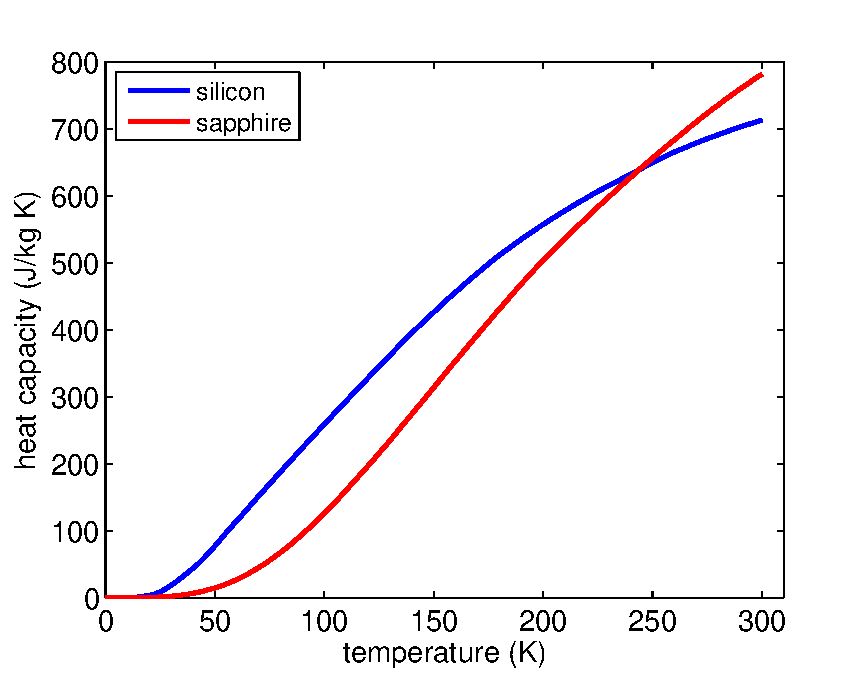
\includegraphics[width=0.49\linewidth]{./Sec_Suspensions/Figures/Cp_T.pdf} \label{fig:heat_cap}}
\subfigure[Coefficient of thermal expansion (\cite{Touloukian1970_alpha_metal,Touloukian1970_alpha_nonmetal}).]{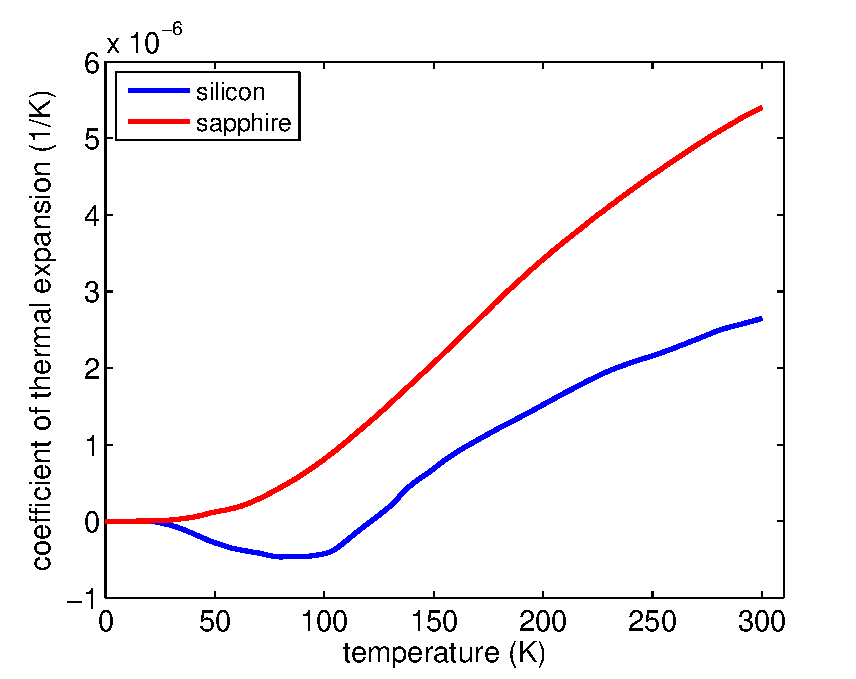
\includegraphics[width=0.49\linewidth]{./Sec_Suspensions/Figures/alpha_T.pdf} \label{fig:alpha_T}}
\end{center}
\caption{Heat capacity and coefficient of thermal expansion for silicon and sapphire as a function of temperature. The heat capacity of both materials follows the predictions of the Debye-law that states a $\mathrm{T^3}$ behaviour. The coefficient of thermal expansion also decreases with decreasing temperature. Silicon shows a special behaviour having two distinct temperatures (around 18\,K and 125\,K) where the coefficient of thermal expansion vanishes.}
\end{figure}

The CTE determines the level of thermo-elastic loss and thus thermo-elastic noise of the suspension elements. Here, fluctuations of the local temperature is directly transferred into a position fluctuation by means of the CTE. In order to get a low level of thermo-elastic noise it is necessary to choose an operational temperature that provides a low CTE. Fig.~\ref{fig:alpha_T} summarises the temperature dependence of the CTE for sapphire and silicon. The general trend shows that lower temperatures lead to smaller CTE. Silicon has a special behaviour where the CTE changes its sign at 125\,K and at around 18\,K. Thus, at these two point the CTE is zero and thus the contribution of the thermo-elastic noise in theory zero. However, due to the demand that the suspension element has to extract the residual heat from the optical absorption in the test masses they will not be in a thermal equilibrium and thus a homogeneous temperature distribution along the fibre/ribbon cannot be expected. The lower the overall temperature of the suspension element is the smaller the total thermo-elastic noise contribution. 

Brownian thermal noise of the suspension is strongly dependent on the mechanical loss of the suspension element. The mechanical loss is usually studied by means of a ring-down experiment. For different materials this parameter has been studied in the past in detail (see e.g.~\cite{McGuigan1978,Rowan2000,Rowan2003,Nawrodt2008,Reid2006,Nawrodt_2010_arXiv}) both for bulk materials (see section~\ref{sec:material}) and suspension elements made from fused silica (see e.g.\ ~\cite{Rowan1997,Heptonstall2006,Gretarrson1999,Penn2001,Penn2006}). There is only little known about the intrinsic loss of silicon or sapphire samples with dimensions close to the ones used in suspension elements. Silicon studies have revealed that thin silicon flexures can reach a mechanical loss as low as $4.4\times10^{-7}$ at about 80\,K~\cite{Reid2006} and even $3.5\times10^{-8}$ at around 10\,K~\cite{Nawrodt_2010_arXiv}. The mechanical loss of a thin silicon flexure studied down to 10\,K is presented in figure~\ref{fig:loss_Si_flexure}. The mechanical loss drops by around 3 orders of magnitude during cooling from room temperature to below 10\,K. The behaviour of the mechanical loss is dominated by the thermo-elastic damping at higher temperatures. At around 125\,K the vanishing CTE causes a dip in the mechanical loss curve.

\begin{figure}[!h]
\begin{center}
\subfigure[]{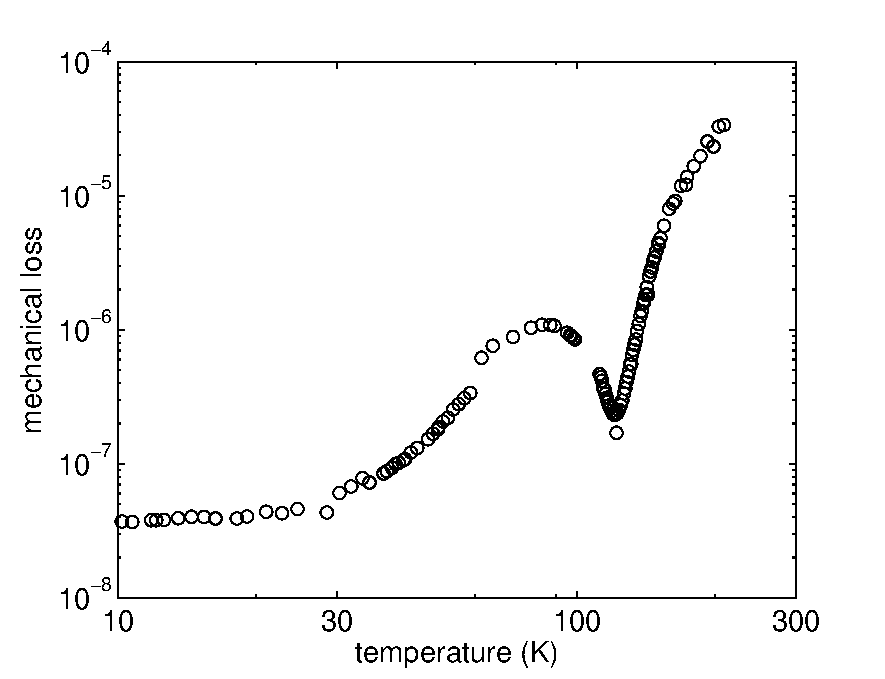
\includegraphics[width=0.49\linewidth]{./Sec_Suspensions/Figures/Si_flexure_loss.pdf} \label{fig:loss_Si_flexure}}
\subfigure[]{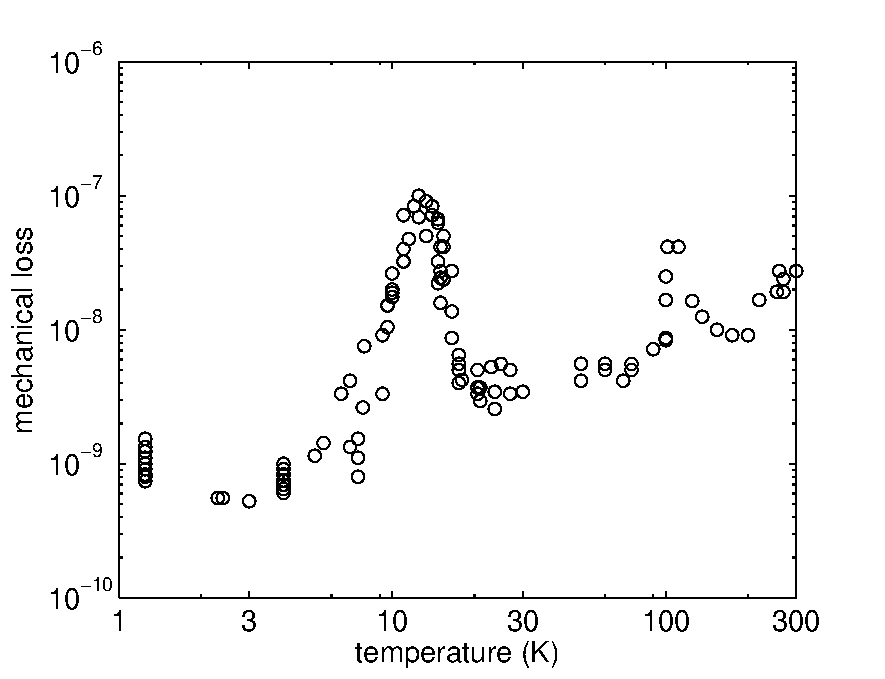
\includegraphics[width=0.49\linewidth]{./Sec_Suspensions/Figures/Si_bulk_loss.pdf} \label{fig:loss_Si_bulk}}
\end{center}
\caption{Comparison of the mechanical loss of silicon. (a)~-- silicon flexures \cite{Nawrodt_2010_arXiv} at 19.6\,kHz, (b)~-- bulk silicon \cite{McGuigan1978}. Loss peaks in the bulk material measurement are associated with impurity induced losses that can be avoided.}
\end{figure}

Compared to the mechanical loss of bulk silicon this value is slightly higher. The reason for this higher mechanical loss is currently assumed to be associated with surface losses. The investigation of the origin of these surface losses is within the focus of the current R\&D (see section~\ref{sec:technologies}). Losses of about $10^{-8}$ are believed to be within the range of achievable values by the time ET will be built.

\begin{figure}[!h]
\begin{center}
\subfigure[300\,K.]{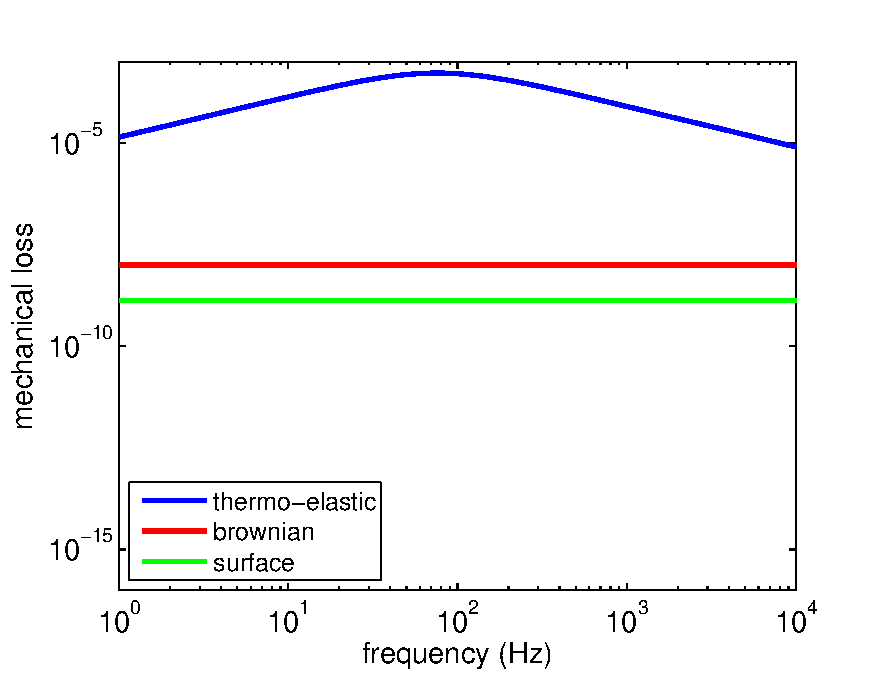
\includegraphics[width=0.49\linewidth]{./Sec_Suspensions/Figures/susp_loss_300K.pdf} \label{fig:susp_loss_300K}}
\subfigure[10\,K.]{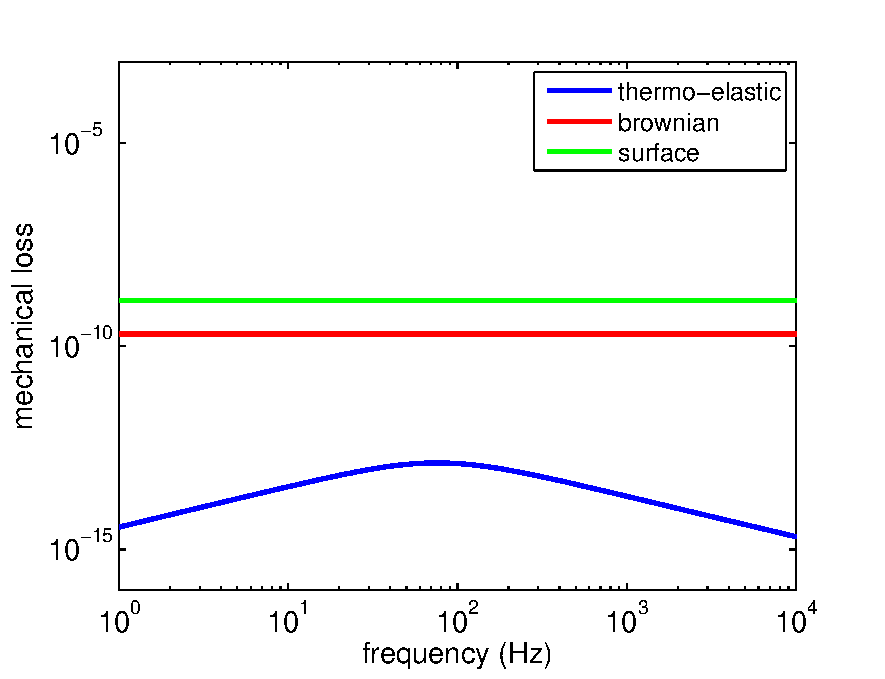
\includegraphics[width=0.49\linewidth]{./Sec_Suspensions/Figures/susp_loss_10K.pdf} \label{fig:susp_loss_10K}}
\end{center}
\caption{Comparison of the loss contributions of a suspension fibre with a diameter of 3\,mm that has been proposed to be used for the low frequency detector of ET.}
\label{fig:susp_loss}
\end{figure}

Figure~\ref{fig:susp_loss} summarises the different loss contributions of a fibre suspension element typically needed for ET. While at room temperature thermo-elastic loss contributions dominate the low temperature suspension element is limited by intrinsic mechanical loss and surface loss which is assumed to be frequency independent as a first approximation. Both, the mechanical loss as well as the surface loss of silicon structures are within ongoing investigations (see Sec.\,\ref{sec:si_surface_loss}). For the ET design a conservative estimate fof $1\times10^{-8}$ was assumed for typical suspension elements. However, each improvement in the mechanical loss or the surface loss of the suspension elements leads to further lowering of suspension thermal noise.

Currently, there are two possible techniques under investigation for the fabrication of silicon suspension elements. The first technique is the so-called micro-pulling technique~\cite{articolofibresil}. Here, a thin fibre with typical diameters in the lower millimetre range is drawn from a silicon melt. The fabricated fibres are not perfectly single crystalline - but recent work has improved the crystallinity of the fibres. Currently, these fibres are produces with a length of 30\,cm for the initial investigations. In principle there is no limit for the maximum achievable length and thus this technique is promising to be used for the low temperature suspensions for ET. For technical details of the fibre pulling technique see the section~\ref{sec:crystal-production}.

The second attempt is to use suspension structures etched out of single crystals or wafers. This technique provides suspension elements with a rectangular or quadratic cross section due to selective etching of the crystalline silicon in different directions. This technique utilises different well established processes from the fabrications of MEMS (micro-electro mechanical systems). A very well known and accurate silicon processing exists to fabricate structures out of crystalline silicon. Figure~\ref{fig:Si_canti} shows such a typical element. A thin silicon flexure was fabricated from Si-wafers with a rectangular cross-section. The thickness of the flexure is in the range of a few 10 microns while the width and the length are in the range from 5 to 70\,mm. The selective etching technique is just limited by the wafer size and in principle it is possible to create much longer elements. These structures have been used to investigate the intrinsic losses of silicon flexures~\cite{Reid2006} as well as intrinsic losses of coating materials applied to them~\cite{Martin2008,Martin2009,Martin2010}.

\begin{figure}[!h]
\begin{center}
\subfigure[]{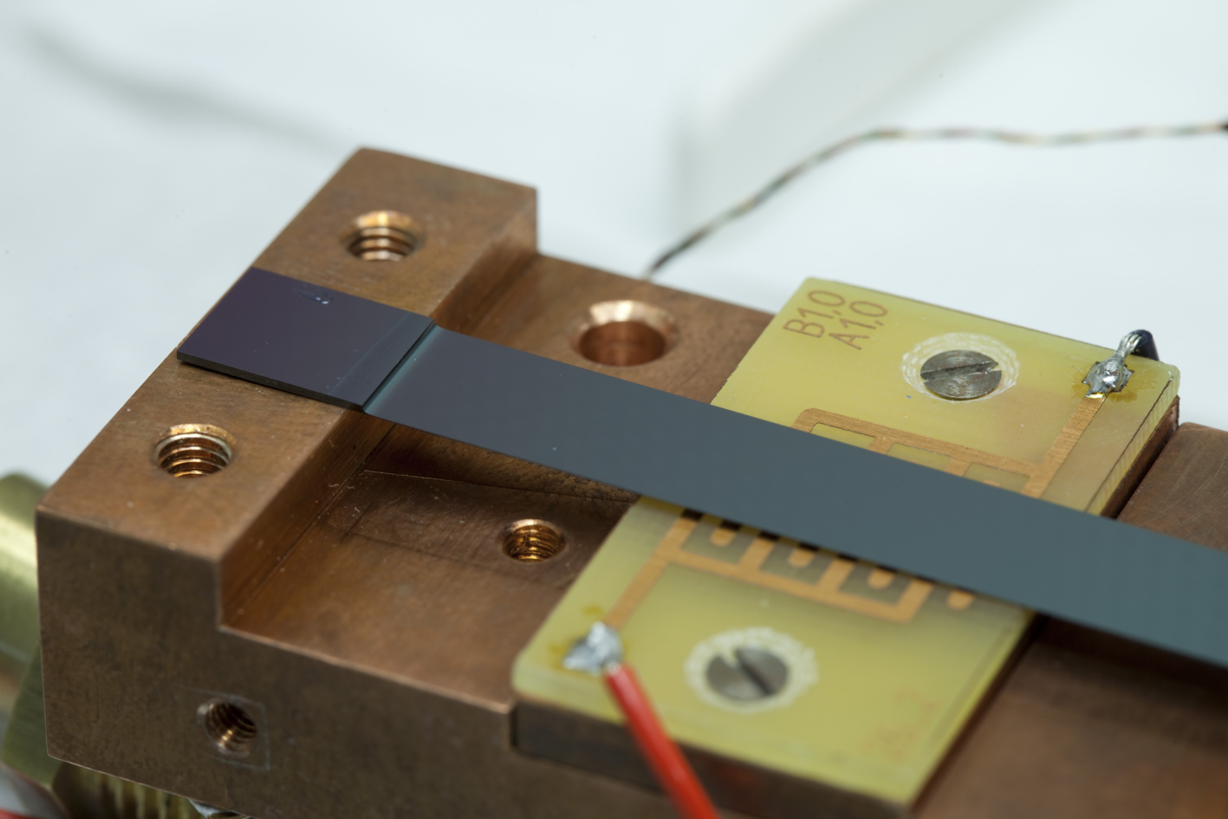
\includegraphics[width=0.49\linewidth]{./Sec_Suspensions/Figures/Si_flexure.png} \label{fig:Si_canti}}
\subfigure[]{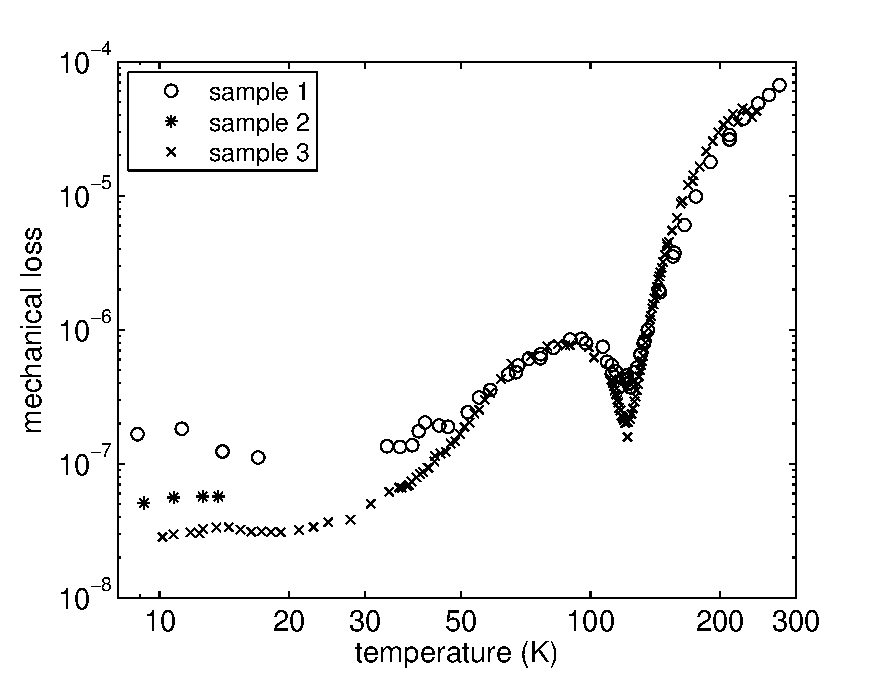
\includegraphics[width=0.49\linewidth]{./Sec_Suspensions/Figures/Si_flexure_loss_rough.pdf} \label{fig:flexure_loss}}
\end{center}
\caption{(a) Silicon flexure etched out of a silicon wafer. (b) - Mechanical loss obtained from different surface qualities. Depending on the surface preparation different roughnesses have been obtained (sample 1 - 330\,nm, sample 2 - 33\,nm, sample 3 - 6\,nm; RMS roughness over 100\,$\mathrm{\mu m}$).}
\end{figure}

There exist different etching techniques to fabricate such structures. The most frequently used ones are selective wet chemical etching and dry etching. These two technique provide different surface qualities strongly depending on the exact process parameters. Fig.~\ref{fig:flexure_loss} indicates that the minimum obtainable loss from these devices at low temperatures is strongly surface dependent. The origin of the surface losses in silicon are so far not fully understood and within the focus of the research carried out by several institutions involved in this design study (see section~\ref{sec:si_surface_loss}).

The promising flexure structures that are currently available and that are showing very low mechanical losses have an anisotropic stiffness due to their geometry. While in one direction the suspension element is soft (e.g.\ in beam direction) it is very hard in the perpendicular direction. This might lead to problems in the control of the interferometer (see section~\ref{sec:local_control}). Therefore, the investigation of the fabrication of crystalline fibres as well as novel control strategies including anisotropic properties need to be done. A summary of ongoing R\&D activities regarding the suspension elements can be found in section~\ref{sec:technologies}.
\FloatBarrier



\subsubsection{Suspension thermal noise model}
\label{sec:thermal_noise}
%\emph{Author: P.\ Puppo}

%%%%%%%% box The thermal Noise
\etbox{h}{Thermal}{Thermal noise}{Thermal noise is due to the brownian motion of the molecules of a system continuously exchanging thermal energy with the environment at thermal equilibrium, via the dissipation mechanisms. As a result the thermal noise of a macroscopic body is a fluctuation of its position which can be formally described as a displacement spectrum using the fluctuation dissipation theorem (FDT). For this reason temperature and mechanical losses are important parameters for the entity of such a noise.}
%%%%%%%%%%

Thermal noise of the mirror suspensions is one of the intrinsic limits to the detector sensitivity in the low frequency range below $10 \ Hz$.
To calculate the thermal noise curve of this system along the horizontal and vertical degrees of freedom, we can write the 
Lagrangian by supposing the 3 elements as point-like masses so that the Virgo-like last stage suspension is a cascade of three pendula:  
 to the first pendulum (the marionette, $M_1$) the mirror $M_2$ and the recoil mass $M_3$ are hung as branches (see figure~\ref{LSSfig}). 
As a consequence the rotations about the coordinate axes are not included.  This choice can be reasonable if we suppose a 
negligible coupling of such degrees of freedom with the interferometer output coordinate. 

The study of the thermal noise of this system can be carried on by using two different methods: 
the Fluctuation Dissipation Theorem (FDT)  and the modal expansion methods \cite{PPP2009,ThModal}. 
For both these methods we write the motion equations from the Lagrangian and the dissipation functions. 

The FDT approach uses the mechanical impedance matrix $\hat{Z}$. The spectral density of the thermal displacement noise of the $i_{th}$ 
mass of the system, is given by the formula:
\begin{equation}
S_{therm}^i(\omega)=\frac{4 k_b T}{\omega^2}  {\cal{R}}e\left\{(\hat{Z}^{-1})_{ii}(\omega)\right\}
\label{eq_FDT}
\end{equation}
where $k_b$ is the Boltzmann constant and $T$ is the temperature of the system.
In the modal expansion method, the motion equations are diagonalised and the normal modes frequencies and coordinates are found in function of the free oscillators ones.
In this way it is possible to infer the frequencies, the displacements and the losses of each pendulum from the measured ones on the system modes. 
The main difference between this model and the FDT treatment, is that it allows us to insert the Langevin stochastic thermal forces independently acting on 
each pendulum. In this way we can study it even in a steady thermal state in which every oscillator has a different stationary temperature. 

This behaviour can be schematised by setting each mass of the $i_{th}$ pendulum at steady thermal state $T_i$ as if it has a constant heat exchange with a thermal bath at the same temperature.  
In this case each pendulum is subject to a different thermal stochastic force:
\begin{equation}
<F_{thi}^2>={\frac{k_b T_i M_i}{\tau_i}}; i=1,2,3
\label{stocforces}
\end{equation}

Using the modal expansion model it can be shown that the thermal displacement noise of the $i_{th}$ mass is also affected by the thermal noise of the other masses 
of the pendulum chain, mainly by the marionette's stage via its dissipation mechanisms.
The FDT and the modal study of the thermal noise lead to the same result if the temperature of the whole suspension is homogeneous. 
A complete study of both the models can be found in the reference \cite{PPP2009}, here we will illustrate the main calculation lines of this method.

\begin{figure}[h]
	\begin{center}
		 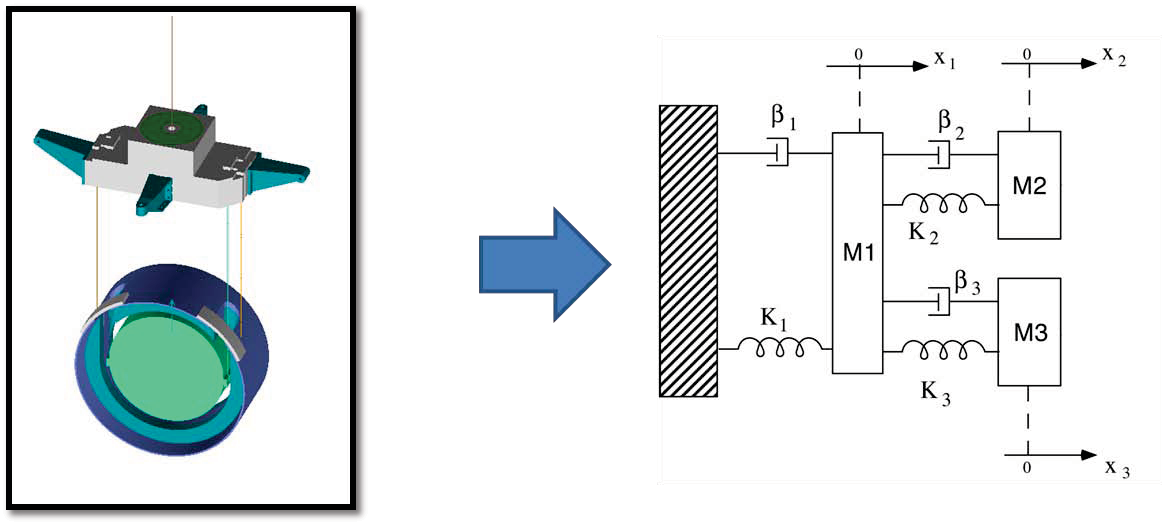
\includegraphics[width=12cm]{Sec_Suspensions/Figures/Branched.pdf}
			\caption{A Virgo-like last stage suspension is a cascade of three pendula.  To the first pendulum (the marionette, $M_1$) the mirror $M_2$ and the recoil mass $M_3$ are hung as branches.  }
\label{branched}
	\end{center}
\end{figure}

\FloatBarrier
\subsubsection{Normal mode formalism} 
In the mode expansion, the eigenvectors of the characteristic matrix of the system are the coordinates $Y_-,Y_0,Y_+$ of the modes and its eigenvalues are the modal frequencies $\omega_-,\omega_0,\omega_+$, thus every normal quantity is a function of the uncoupled ones. Moreover, the stochastic normal forces $F_-, F_0, F_+$, acting on each mode, are found in function of the uncoupled ones \cite{PPP2009}.

Within this formalism, the mirror coordinate $X_2$ is expressed in terms of the normal eigenvectors and its thermal noise is calculated with its power spectrum. We find:  
\begin{equation}
  \left\langle {{X_{th2}}{{(\omega )}^2}} \right\rangle  = \left\langle {{F_{th1}}^2} \right\rangle {\left| {{T_{n1}}(\omega )} \right|^2} + \left\langle {{F_{th2}}^2} \right\rangle {\left| {{T_{n2}}(\omega )} \right|^2} + \left\langle {{F_{th3}}^2} \right\rangle {\left| {{T_{n3}}(\omega )} \right|^2} \\ 
\label{eq12}
\end{equation}
where $T_{ni}(\omega)$ are generalized transfer functions depending on the uncoupled mechanical parameters of the pendula~\cite{PPP2009}.

This result is fully equivalent to the FDT calculation shown in equation~(\ref{eq_FDT}) at homogenous temperature, however the explicit dependance on the temperatures $T_i$ (in the $ \left\langle {{F_{thi}}^2} \right\rangle$ given by the equation \ref{stocforces}) is the new result which permits to calculate the thermal noise of a suspension at a thermal steady state but with the stages at different temperatures.
\FloatBarrier
\subsubsection{Thermal noise computation of LSS for the LF interferometer}
Using equation \ref{eq12}, we have studied the thermal noise of a Virgo-like last stage suspension for the LF cryogenic interferometer characterised by the parameters summarised in table~\ref{Parametri}. The working temperature at the mirror level is 10\,K, corresponding to the minimum mechanical losses of the coatings ($\mathrm{Ti:Ta_2O_5}$, see section~\ref{sec:optcomps}). The material for the mirror bulk and its suspension wires is silicon with a loss angle of $10^{-8}$ (see sections~\ref{sec:mat_lss} and \ref{sec:optcomps}). 
The marionette and the RM masses have been chosen in order to reduce the marionette recoil effects as much as possible. For this reason the marionette mass must be the sum of the masses of the mirror and the RM at least. 
The materials used for making the suspension wires are silicon for the RM and Ti6Al4V alloy for the marionette with a loss angle of $10^{-5}$ \cite{tialloy}; their length is $2 \ m$. The diameter of the silicon wire has been chosen to be $3 \ mm$: with this value the temperatures of the marionette and the mirror in the steady state are $2 \ K$ and  $10 \ K$ respectively with a silicon wire having an thermal conductivity which is more than an order of magnitude worst than that one of the highly pure material (with 1000 W/K/m mean value see section \ref{sec:mat_lss} ). These value can take into account the presence of the thermal resistances due to the contacts between the mirror wire and the suspension system.

\begin{table}
\begin{center}
\begin{tabular}{|c|c|c|c|}
\hline
				&Marionetta	&Recoil Mass 	& Mirror\\
\hline
Masses for ETDLF (kg)			&422		&211			&211\\
\hline
Wire Diameter (mm)	&3		&3			&3\\
\hline
Wire length (m)	&2		&2			&2\\
\hline
Wire Material		&Ti6Al4V	&Silicon		&Silicon\\
\hline
Loss Angle		&$10^{-5}$&$10^{-8}$&$10^{-8}$\\
\hline
Temperature (K)		&2	&10		&10\\
\hline
\end{tabular}
\caption{Parameters used in the design of the mirror last stage suspension for the LF interferometer.}
\label{Parametri}
\end{center}
\end{table}


\begin{figure}[htbp]
\begin{center}
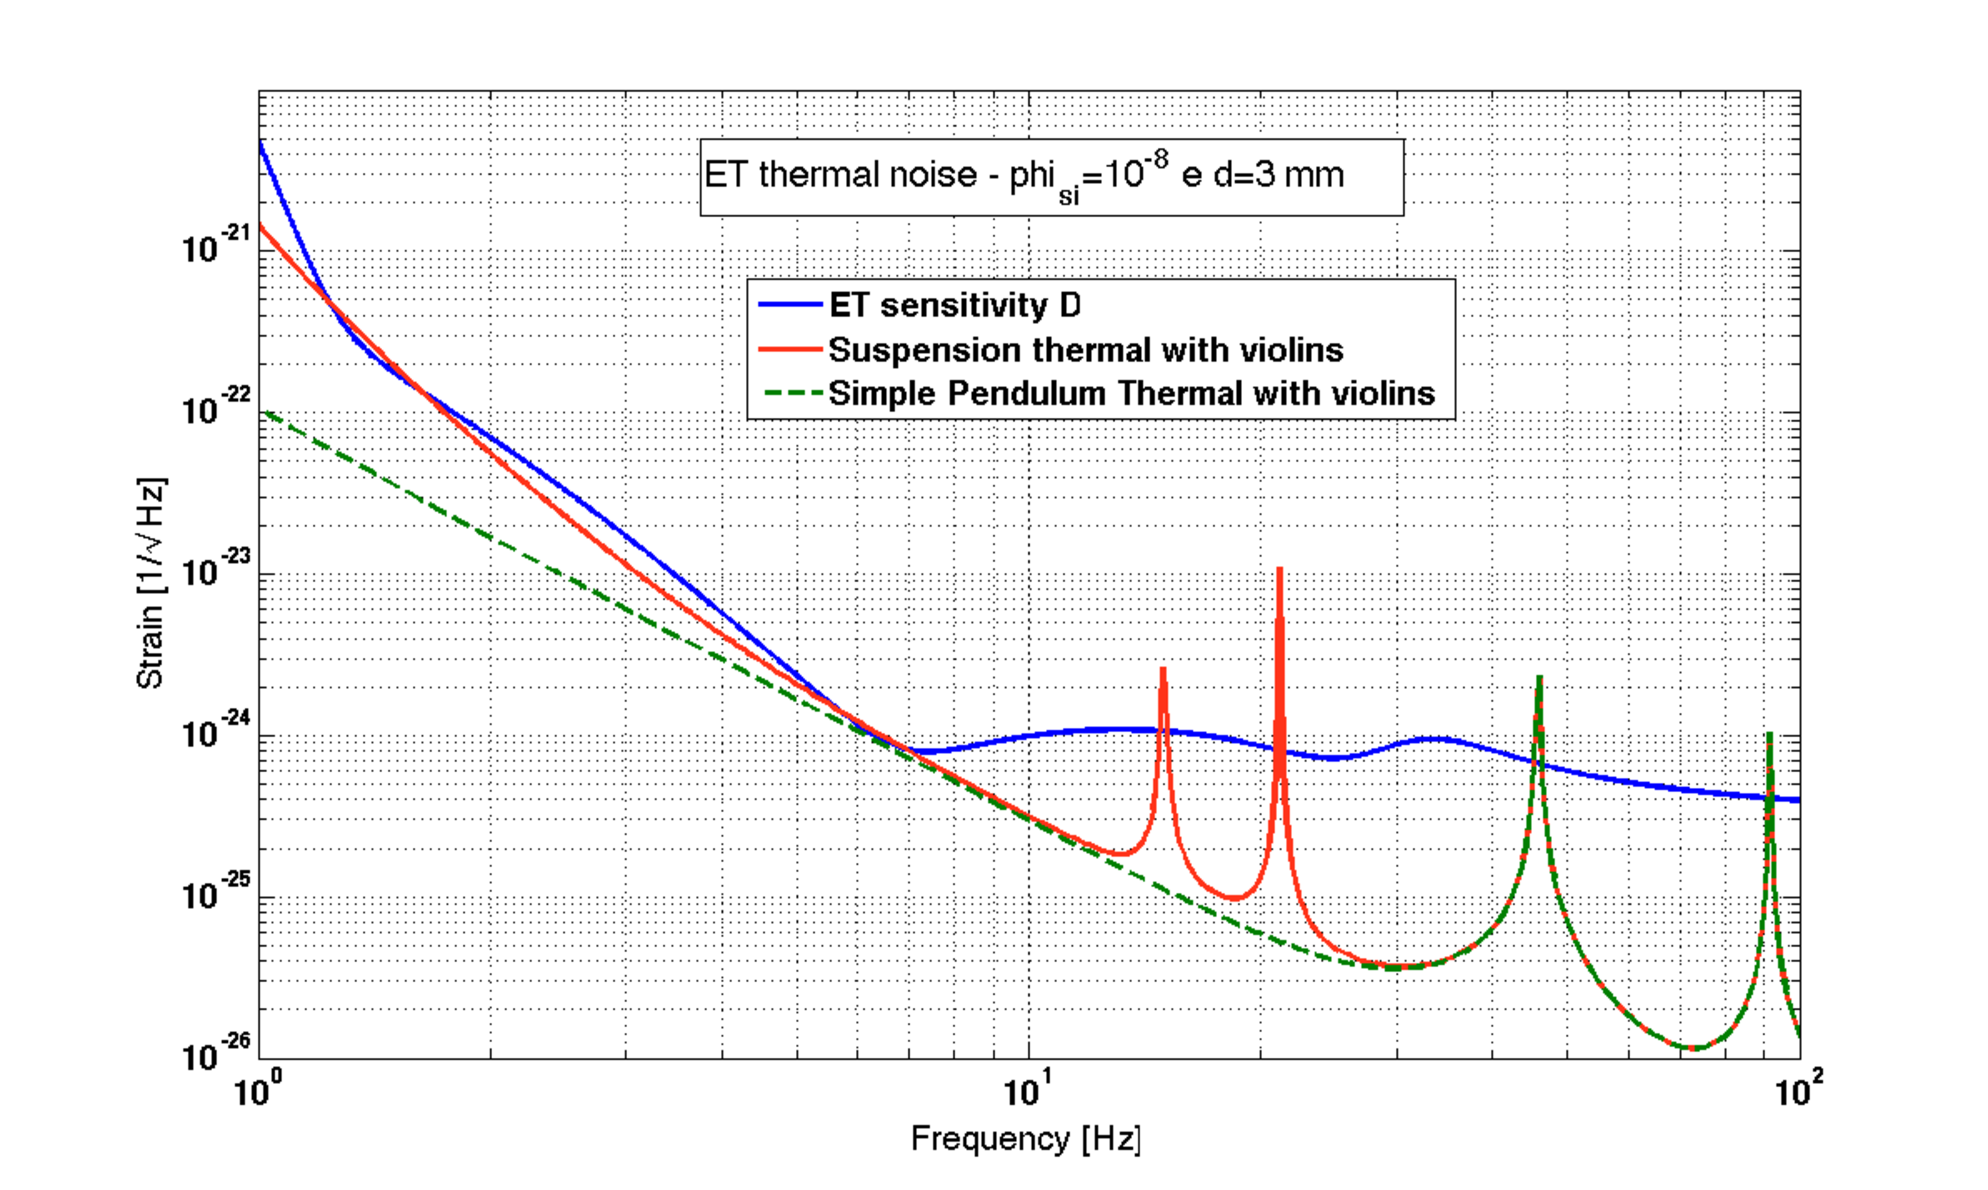
\includegraphics[width=13cm]{Sec_Suspensions/Figures/ETDLFthermvsETDLFsens3.pdf}
\caption{ET-D-LF sensitivity curve (blue) compared with the suspension thermal noise calculated with the parameters of the table \ref{Parametri} (red) and with the simple pendulum thermal noise (dashed green).}
\label{fig:Sensitivity_ET}
\end{center}
\end{figure}

The obtained thermal noise curves have been compared with the ET-D goal sensitivity curve where the power stored in the cavities of the cryogenic interferometer $18 \ kW$. The results are sketched in figure \ref{fig:Sensitivity_ET} where the obtained suspension thermal noise is also compared with the simple pendulum one. It can be noticed that, below $10 ~ Hz$, the overall contribution of the whole last stage suspension system is higher than that one of the simple pendulum, and it must be taken into account for a correct optimisation of the sensitivity curve in this range of frequency.

\FloatBarrier
\subsubsection{The payload of the HF interferometer}
\label{sec:HF-interferometer}

%\emph{
%Author(s): P.\ Puppo, F.\ Ricci}


The LSS design of ET-HF  is greatly based on the experience on Virgo and Advanced Virgo.  The  marionette will be almost the same as in Advanced Virgo, while the  recoil mass design of can be adapted to different mirrors lengths. We will   accommodate in it the  thermo  compensation plate (CP),  an other optical element  s essential for compensating the thermal lensing induced in the test mass mirror by the huge laser power stored in the HF Fabry-Perot cavities. 
A Marionette Recoil Mass is being developed: facilitates installation and operation for large diameter mirrors, could improve thermal noise matching for Test Mass Mirrors, it is necessary for larger mirrors (i.e.\ the BS). 

The materials with low acoustic loss for the mirror and for the suspension is crucial to reduce the thermal nose contribution to the sensitivity of ET-HF. 
In the marionette design the requirements for cleanliness, vacuum compatibility, mechanical precision, magnetic and electrical properties apply. Moreover several new aspects must be considered: the use of the fused silica fibres and the change of geometry of the mirror. 


Moreover, monolithic suspensions currently being tested in GEO and with a 21 kg mirrors in Virgo should be developed for a 200 kg test mass (\ref{sec:bonding}).
In the case of the monolithic suspensions, the silica wires must be attached to the marionette by a new kind of clamps which must not introduce further mechanical losses in the interface between the silica and the marionette surface. 
These new clamps have to be placed in such a way the fibre bending point lays on the horizontal plane passing through the centre of mass of the marionette to minimise the coupling between different degrees of freedom. As the wire bending section is different by the clamping section, because of the tapered fibre tip (see section \ref{sec:bonding}), this is carefully taken into account in the new design. 
The coupling between the marionette and the fibre also influences the mounting procedure of the payload and consequently the new assembly tool design. Moreover the change of the position of suspension wires of the new reference mass, and, in case of need, of the balancing motor, are taken into account. 

In the new reference mass (RM)  design the requirements for cleanliness, vacuum compatibility, mechanical precision and magnetic and electrical properties apply.  The new design takes into account the bigger thickness and mass of the mirrors, the implementation of the mirror control and the thermal compensation system. 

The actuators have to be designed to fulfil the displacement requirements for the locking purposes and consequently are related to the optical configuration. There are two different options for the mirror actuation by the reaction mass: the coil-magnet actuators and the electrostatic actuators. We present them in the  sections \ref{sec:em_actuator}, \ref{sec:electrostatic}.

The RM surrounds the mirror in order to protect it by accidents and hosts its actuators. It is equipped with safety stops designed taking into account the different shape and increased mass of the mirrors suspended with a monolithic structure. 
The design is conceived to host the ring heater and compensation plate foreseen in the thermal compensation system. To this aim, the dielectric parts of the RM must work at high temperature because of the possible contact with the heaters. 
The presence of a compensation plate could deeply affect the dynamical behaviour of the last stage suspension: the centres of mass of mirror and RM must coincide to reduce the coupling among the various degrees of freedom. The structure required to carry the compensation plate will make more difficult to satisfy this requirement. 

In the case of the coil-magnet actuation (see section \ref{sec:em_actuator}), here assumed as the reference solution,  it is necessary to design RM as made of  a dielectric material to avoid eddy current dissipation and magnetisation effects. The mechanical strength of the new insulating material must allow to use the reaction mass also as a safety structure for the mirror.

The dielectric material must be chosen to be UHV and cleanliness compatible. However,  it could produce   electrostatic charge on the mirror  by friction with the RM. A solution can be the use of dielectric materials having also a resistivity value sufficient to avoid the formation of stray currents but reduces the presence of static charges. A possible choice is the TecaPeek CF30, a kind of polymeric plastic, loaded by carbon and grafite particles to increase its density and have a slight electrical conductivity which is useful to avoid the static charges formation. 
 
\begin{figure}[htbp]
\begin{center}
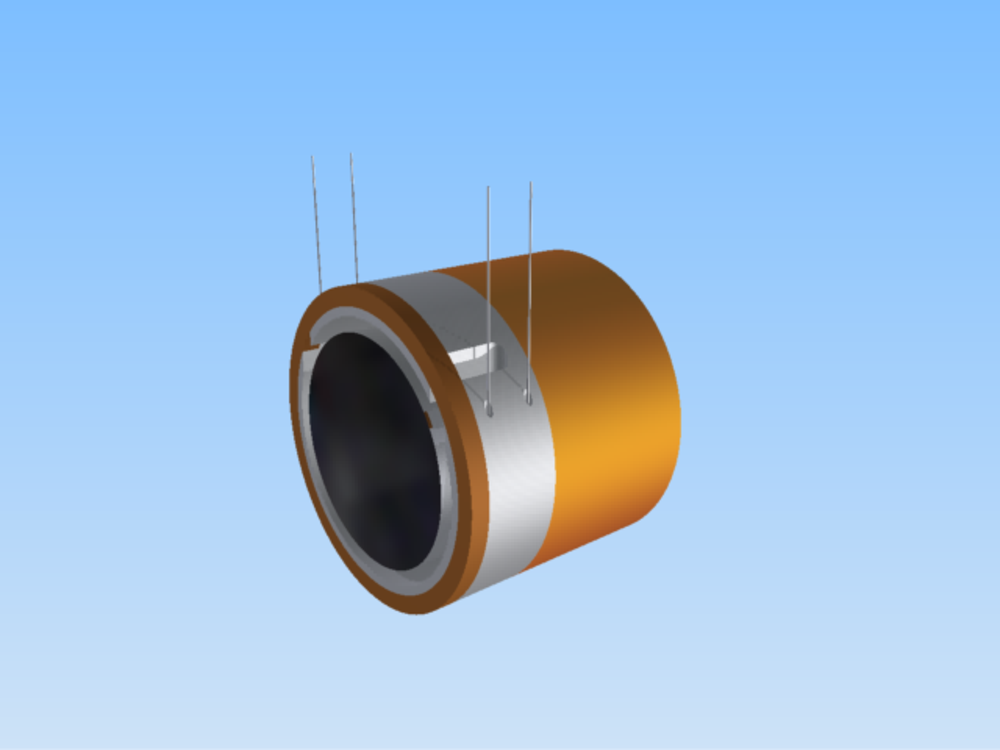
\includegraphics[width=0.5\textwidth]{Sec_Suspensions/Figures/ET_RM.pdf}
\caption{\label{fig:RM} Schematic picture of the new mirror reaction mass. The various colors indicate the different materials used.}
\label{fig:ET_RM}
\end{center}
\end{figure}
%\begin{figure}[htbp]
%\begin{center}
%\includegraphics[width=0.5\textwidth]{Sec_Suspensions/Figures/Advsusp.pdf}
%\caption{\label{fig:RM}\sf Schematic picture of the mirror monolithic suspension system.}
%\label{fig:ET_monsosp}
%\end{center}
%\end{figure}



The ET configuration for the last stage suspension system  can include a new element: the Marionette Reference Mass (MRM). The new element  will permit

\begin{itemize}
\item	to suspend a larger diameter mirror avoiding any mechanical interference between the marionette and the pots installed on the separating roof of the Ultra High Vacuum (UHV) chamber;
\item	to simplify the payload installation and its preliminary alignment procedure;
\item	to guarantee a high level of mirror cleanness without spoiling mechanical performance of the suspension system.
\end{itemize}

\noindent
The MRM will be suspended within the UHV chamber between the marionette and the last filter of the \emph{Superattenuator} chain. It will host the actuator coils for steering the marionette. In this way a more compact design of the payload will be conceived and the IVC structure could be revised to accommodate a mechanical filtering system for the air flow entering within the UHV chamber. 
Following these project guidelines, the payload integration on the suspension system will benefit of:  

\begin{itemize}
\item	a wider clearance for the monolithic payload assembly, including the possibility to install a larger diameter mirrors;
\item	a compact payload, which is  pre-aligned before the final installation in the vacuum chamber. In this way it is possible to reduce the time spent by the operators for the installation and positioning;, which is the main cause of environmental pollution;
\item	a quasi-laminar flow of clean air within the UHV chamber volume to be used during the assembly phase (TBC).
\end{itemize}



Monolithic fused silica (FS) suspension of the four 200 kg Fabry-Perot cavity mirrors will be realised for ET HF, exploiting the experience achieved developing the Virgo+ payload. The optimal geometry and technology is being pursued with the objectives of minimising the pendulum thermal noise, fulfilling the requirements for an optimal control of the test mass, ensuring safety and reliability. For Virgo+ a large amount of work has been made to reduce the risk in the welding procedure. The fibres (once welded directly to the mirror) are now welded to intermediate components (called ears) silicate bonded to the lateral flats of the test mass (see figure \ref{fig:ET_HF_mirror}). The former procedure induced a lot of thermal stress on the bonded surfaces that could damage the silicate bonding and eventually break it. Another problem is that the fibres pass through a dangerous manipulation procedure that can open cracks on their surface decreasing their breaking strength. To recover these problems a new technique has been developed: two lateral supports with vertical grooves are attached using silicate bonding to the mirror lateral flats.  In parallel, a fused silica bar is previously welded to an upper clamp and a lower anchor and then the fibre is produced. The fibres are then placed in position clamping the upper part to the marionette and inserting the lower anchor below the lateral supports bonded to the mirror. In the end the anchor and the supports are bonded together through silicate bonding or {\it water glass}.
Although this solution has been successfully implemented for Virgo it would be easier (and with lower mechanical dissipation) to avoid the lateral bonding of the supports to the mirror. 

\begin{figure}[htbp]
\begin{center}
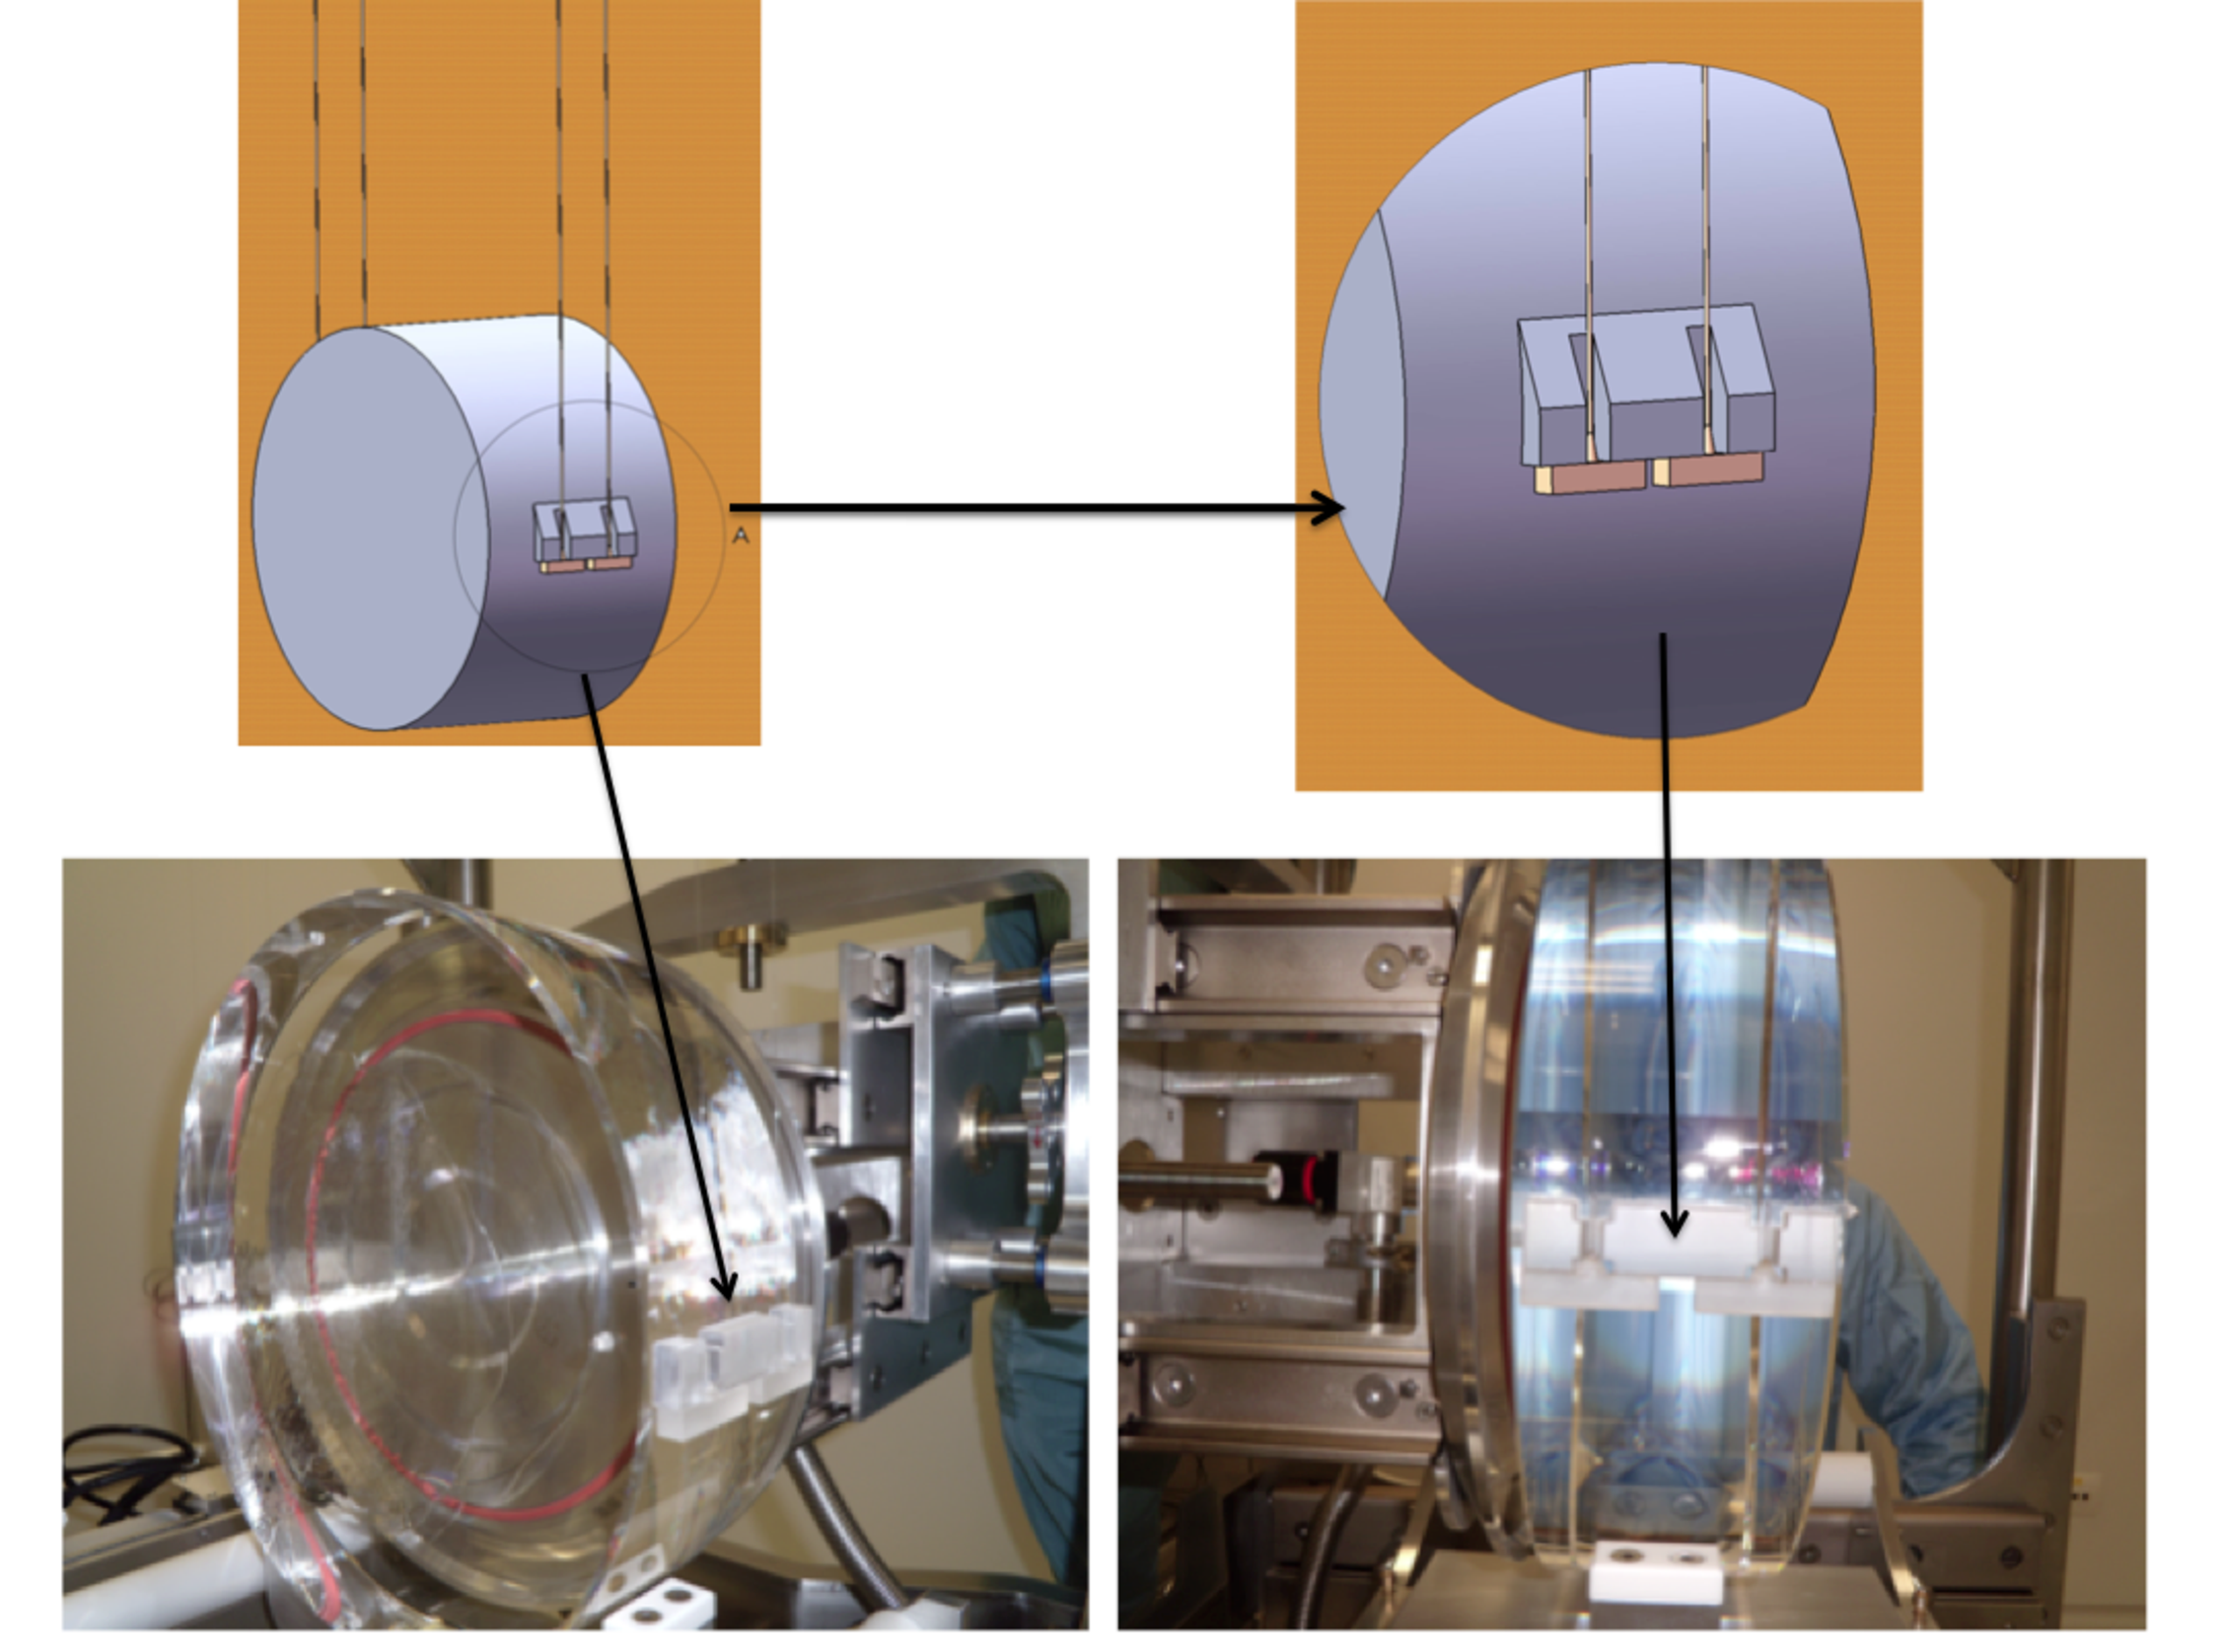
\includegraphics[width=1\textwidth]{Sec_Suspensions/Figures/ET_mirror_HF.pdf}
\caption{On the upper part of the figure we show a scheme of the silica anchor  attached  by the silica bonding.
The various colors indicate the different pieces bonded each other. In the lower part we show  the frontal and  lateral views of a Virgo mirror with the silica anchors already bonded.}
\label{fig:ET_HF_mirror}
\end{center}
\end{figure}


The suspension scheme, already tested inVirgo, will  reduce the most critical part induced by silicate bonding the lateral supports on the lateral mirror flats. The supports can be machined out from the mirror , the lower surface of the support is polished to perform a silicate bonding which will be discussed in the following section~\ref{sec:bonding}.
The suspension scheme proposed is the following:
one fused silica part called "anchor" will be welded to a $\sim 7$\,mm fused silica bar and to an upper clamp.
Using the CO$_2$ laser machine the fibre will be produced from the bar welded to the clamps, the whole clamp-fibre will be placed in position on top to the marionette and on the bottom under the mirror support. The contacting surfaces of the two parts (both with a polishing) will be bonded onsite using the silicate bonding or \emph{water glass} procedure as for Virgo. To this aim it is necessary to find a geometry of the lateral supports easy to machine, and to demonstrate that the surface quality is sufficiently good for thermal noise performances.

The role of the upper clamps coupling with the marionette in order not introduce further frictions and recoil losses is very important. For this purpose a stainless steel box has been carefully designed with the aim to host the silica upper clamp and to attach it to the marionette without introducing further losses. The steel box is formed by two pieces. An external one fastened to the marionette by four screws. An internal one in direct contact with the fused silica and fastened by lateral screws to the external one. The silica core is kept fixed in its box by an upper lid fastened by screws. The steel inner box is also designed as the support of the upper clamp during the fibre pulling (see section~\ref{sec:bonding}) and then is coupled to the tool used to insert the fibre on the marionette lateral side, as foreseen by the assembly procedure.
 

\FloatBarrier
\subsubsection{The payload of the LF interferometer}
\label{sec:LF-interferometer}
%\emph{
%Author(s): R.\ Nawrodt, P.\ Puppo, F.\ Ricci}

Assuming for ET an optic configuration with mirror losses of  the order of $10^{-6}$ and a stored light power of $\sim 18$\,kW, we deal with the need to implement a cryogenic system able to extract  tens of  milliwatts of heat from the mirror during the working steady state. This requirement is compatible  both by defining a cooling strategy based on closed loop cryo-coolers or  by setting up a dedicated liquid helium plant.

Moreover for the employment at low temperature in a GW detector we need to design the suspension system in such a way
\begin{itemize}
\item{to transmit the refrigeration power to the mirror without spoiling the control procedure of the mirror degrees of freedom}
\item{to extract the heating power coming from the laser light in the more efficient and quicker way.}
\end{itemize}

The materials used for building a cryogenic payload must follow these requirements, thus those materials with a very high thermal conductivity, good mechanical and optical properties at low temperature can be taken into account.
Silicon is one of the best candidates both for the mirror and its suspensions in this case, indeed it has a very high thermal conductivity and very low thermal expansion rate. On the other hand the silicon material has very low mechanical losses at cryogenic temperatures.

For this reason in our analysis we have considered a last stage suspension designed as it is in the Virgo interferometer with a silicon mirror suspended to silicon fibres in a monolithic way.

The choice of the materials for building the marionette and the recoil mass must fulfil the requirements given by the work at cryogenic temperatures.
In figure~\ref{fig:scheme} it is shown how a cryogenic suspension should work during the interferometer operation, i.e.\ when the payload has been cooled down and the laser is turned on. The fraction of the laser power, which is  absorbed by the mirror ($\dot{Q}_\text{laser}$),  flows through suspension wires; then it  crosses the marionette clamps and reaches the refrigerating system. To this aim the marionette is directly connected with very efficient, soft heat links to the cooling power.

In a similar way as for the mirror the reaction mass is cooled down via its suspension wires and, if there is not extra thermal input on that, it reaches the thermal equilibrium and acts as a thermal shield for the mirror. The choice of the wires for the recoil mass must fulfil  the request of having a good mechanical and thermal performance. For this reason, the use of a silicon suspension also for this part is a possible option.

In the scheme there is also the reaction mass of the marionette (MRM), absent in the present Virgo-like payloads. This part is an intermediate element between the marionette and last filter of the higher suspension which can act as a mechanic and thermal decoupler and as a thermal shield.
In our study the MRM is not included because it has a negligible contribution to the thermal noise of the mirror \cite{PPP2009}.

The thermal equilibrium is reached when the power extracted by the cooling system is equivalent to that one absorbed by the mirror ($\dot{Q}_\text{abs}=\dot{Q}_\text{coolsys}$). At this condition most part of the power absorbed by the mirror flows through its suspension wires (a small fraction is lost in radiation), and then it is removed by the heat link directly connected to the cooling system.
The equilibrium temperature of the mirror $T_\text{mir}$ can be calculated by the simple analytical model relating it to the temperature of the thermal bath $T_\text{bath}$ of the cooler via the power  flow through the mirror wires:
\begin{equation}
\dot Q_{abs}=  \frac{{{4 \Sigma _w}}}{L}<K_{si}> ({T_\text{bath}} - {T_\text{mir}})\equiv\frac{1}{Z_\text{therm}}\Delta T \\
\label{eq1}
\end{equation}

\noindent 
where we have

\begin{equation}
 <K_{si}> = \frac{1} {{\Delta T}}\int\limits_{{T_\text{bath}}}^{{T_\text{mir}}} {{K_\text{si}}(T) \, dT}
\label{eq1_bis}
\end{equation}

\begin{figure}[htbp]
\begin{center}
 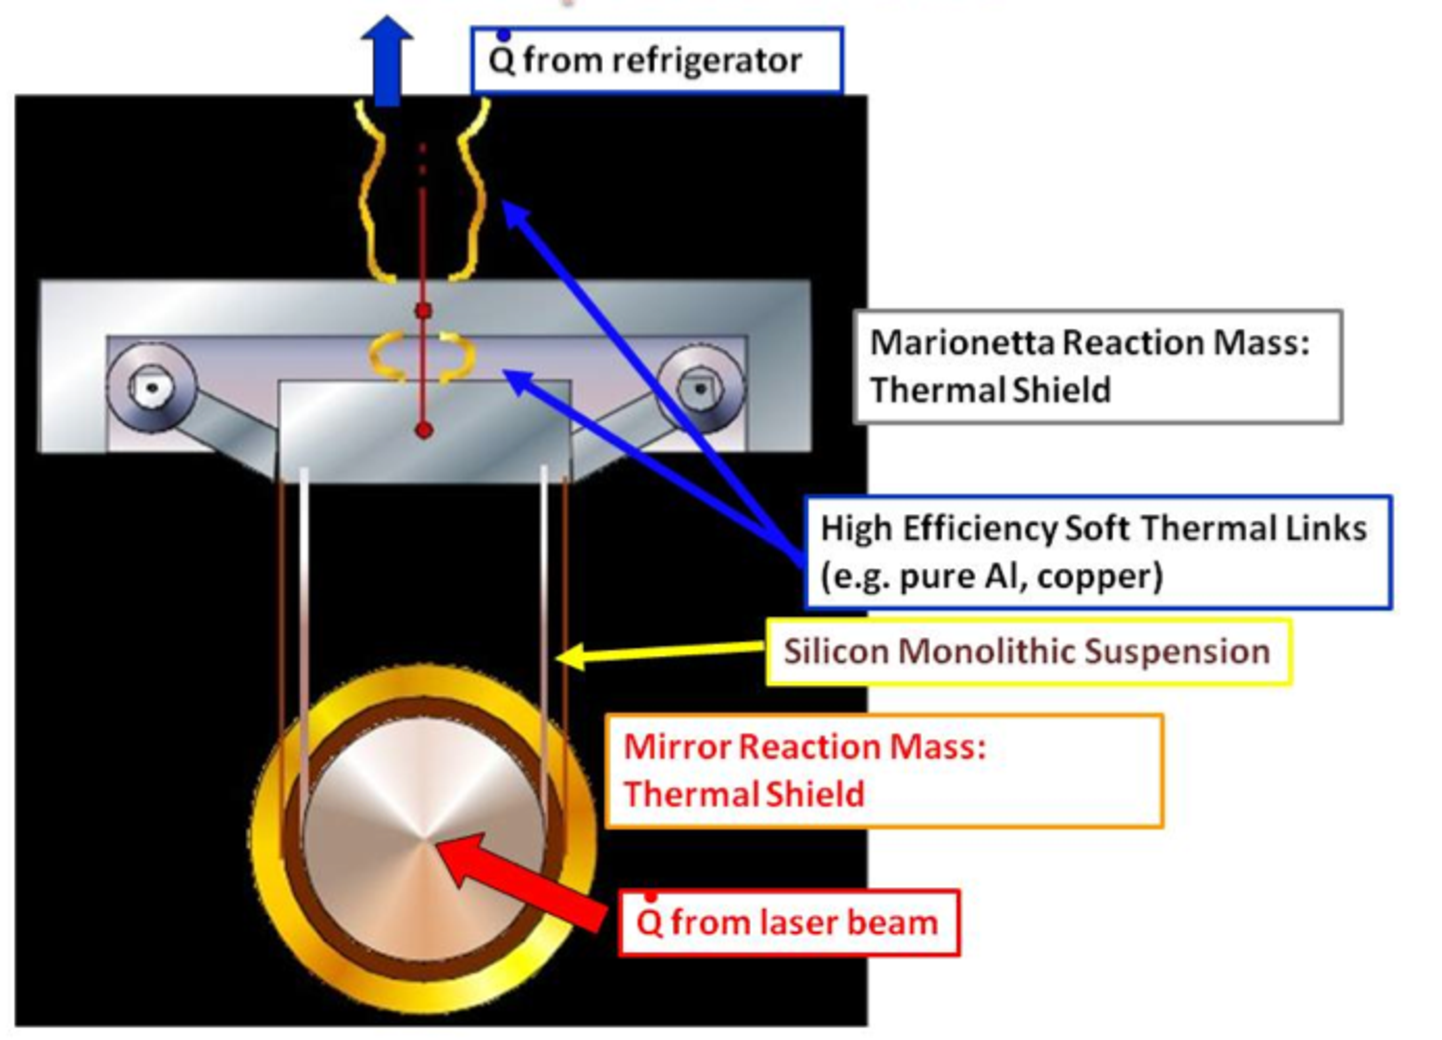
\includegraphics[width=17cm]{Sec_Suspensions/Figures/scheme.pdf}
			\caption{The conceptual scheme for a cryogenic suspension}
\label{fig:scheme}
\end{center}
\end{figure}



\noindent
where $\Sigma_w$ is the wire section, $L$ its length and $K_{si}(T)$ is the thermal conductivity of silicon. For a given thermal input $\dot{Q}_{abs}$, the thermal impedance $Z_{therm}$ is important to yield the final temperature of the mirror: this is the quantity which sets up the performance of our system and influences the choice of the material and of the geometry of the mirror suspension wire.

On the other hand, also the transient phase to reach the steady state must be taken into account, because we do not want too much long cooling times. For this reason the thermal capacity of the whole system plays also a role. Thus the presence of all the masses of the system is important for determining its thermal behaviour. 

To this aim some studies with a finite element simulation have been helpful. 
\begin{figure}
\begin{center}
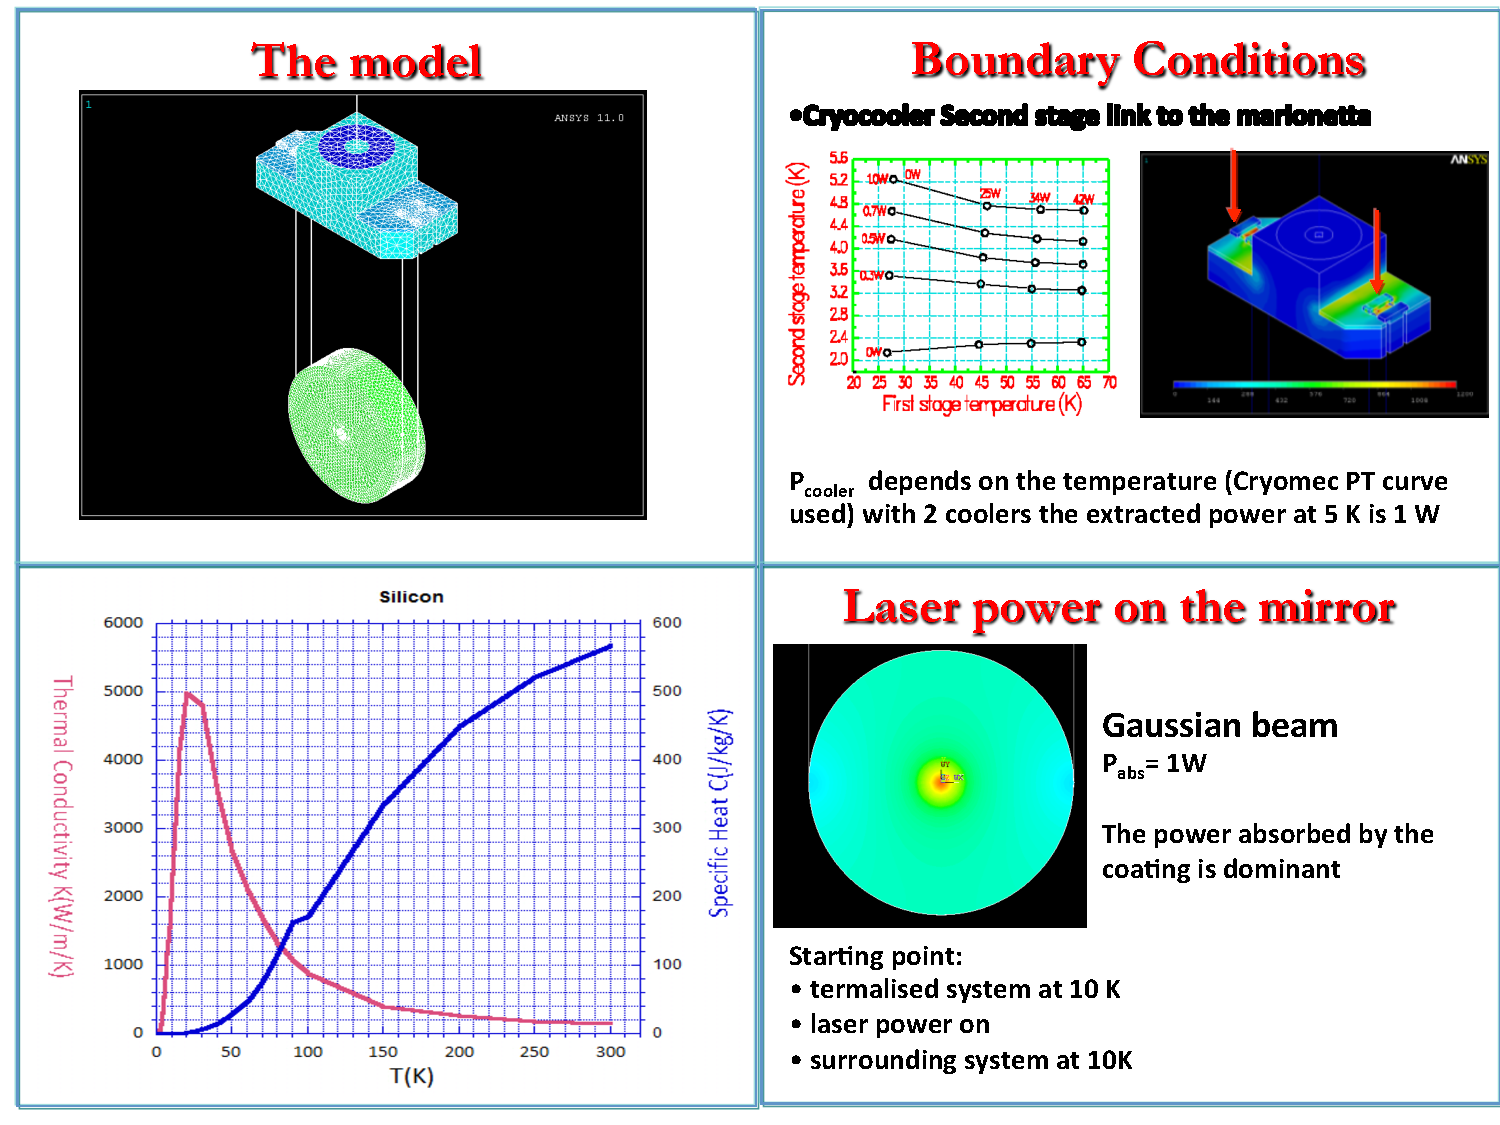
\includegraphics[scale=0.5]{Sec_Suspensions/Figures/Simul.pdf}\\
\caption{The reaction masses are not present in the simulation, their screen effect is simulated by the surround system at 10K.
The marionette arms are not present, silicon thermal properties vs temperature are included in the simulation.}
\label{simul}
\end{center}
\end{figure}
In figure~\ref{simul} it is shown the FEM model developed to perform such a study. The reaction masses are not present, for reasons of computing time, and their screen effect is simulated by the surrounding system at 10\,K. For similar reasons as for the reaction masses, the marionette arms are not present.
The mirror is suspended with a silicon fibre of 1\,mm diameter. The  silicon thermal properties vs temperature are included in the model. The mirror is heated with a power of 1 W distributed around its centre with a gaussian shape to simulate the laser mode. 
The cooling power, directly linked to the marionette, comes from 2 pulse tube cryocoolers with a cooling capacity (W) depending on the temperature: when the last stage of the cryocooler (cold finger) is at 4.5\,K the power is 1\,W, while at 20\,K the cooling power is about 10\,W. At the thermal equilibrium the cold finger temperature is 4.5\,K. A similar behaviour is obtained using the liquid helium with a temperature of the thermal bath of 1.8\,K. 
The simulation results agree with the formula~(\ref{eq1}) when $T_\text{bath}=T_\text{cold finger}$ and give the thermal distribution on the whole payload, as shown in figure~\ref{simul2} where it is evident that the final temperatures of each payload elements are not the same.
 
This result cannot be neglected when the thermal noise of the last stage suspension system is calculated for two main reasons: the thermal properties of the suspension wires change  as the second equation in~(\ref{eq1}) shows; a different temperature upper stage can differently influence,depending on its temperature and mechanical losses, the thermal noise of the mirror. For these main reasons we presented in the previous paragraph~\ref{sec:thermal_noise} the thermal noise model generalised to the case of the stages at different temperatures.

\begin{figure}
\begin{center}
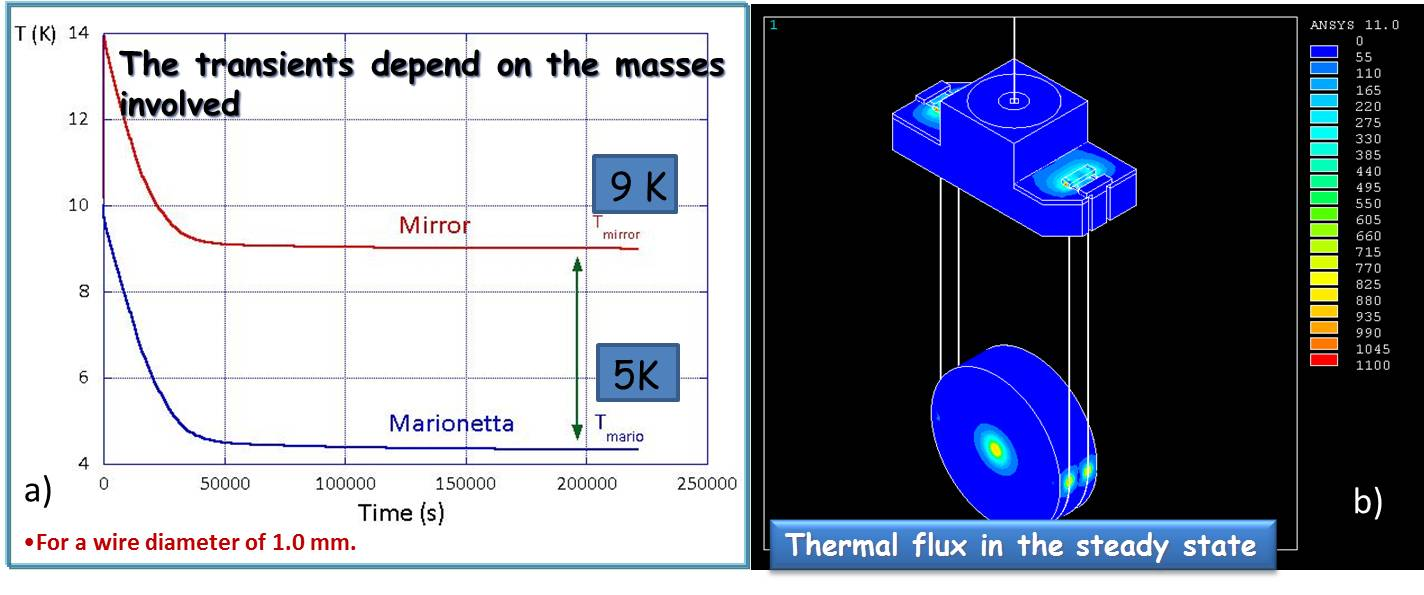
\includegraphics[scale=0.5]{Sec_Suspensions/Figures/Simul2.pdf}\\
\caption{FEM results: a) time evolution of the mirror's and marionette's temperatures, b) thermal distribution on the whole payload.}
\label{simul2}
\end{center}
\end{figure}


\FloatBarrier
\subsubsection{The payload local control for ET}
\label{sec:local_control}
%\emph{
%Author(s)):  F.\ Ricci, E.\ Majorana}

The local control of test masses plays a crucial role in gravitational wave detectors with independent test masses.  
Payload local control system is meant to slow-down and align the test masses as interferometer's mirrors, driving their dynamics within the gain range of automatic error signals (wavefront sensing for angles and locking for longitudinal position). As said, in order to preserve the quasi-inertial state guaranteed at the level of payload suspension point by the Superattenuator, only internal forces should be used. 
The procedure developed in Virgo  should be easily tuneable towards the advanced detector performances; on the other hand the ET digital/analogic chain (Fig.~\ref{overall}) needs to be improved, namely by reducing by more than one order of magnitude the overall low frequency noise re-injection during locking force reallocation to  payload stages. The related R\&D will naturally follow the developments of advanced detector implementations. 

However, the ET system will be complicated by the presence of cryostats surrounding the vacuum chambers hosting the payloads  (Fig.~\ref{overall}), whose design will  not be trivial.
 
\begin{figure}[htbp]
\begin{center}
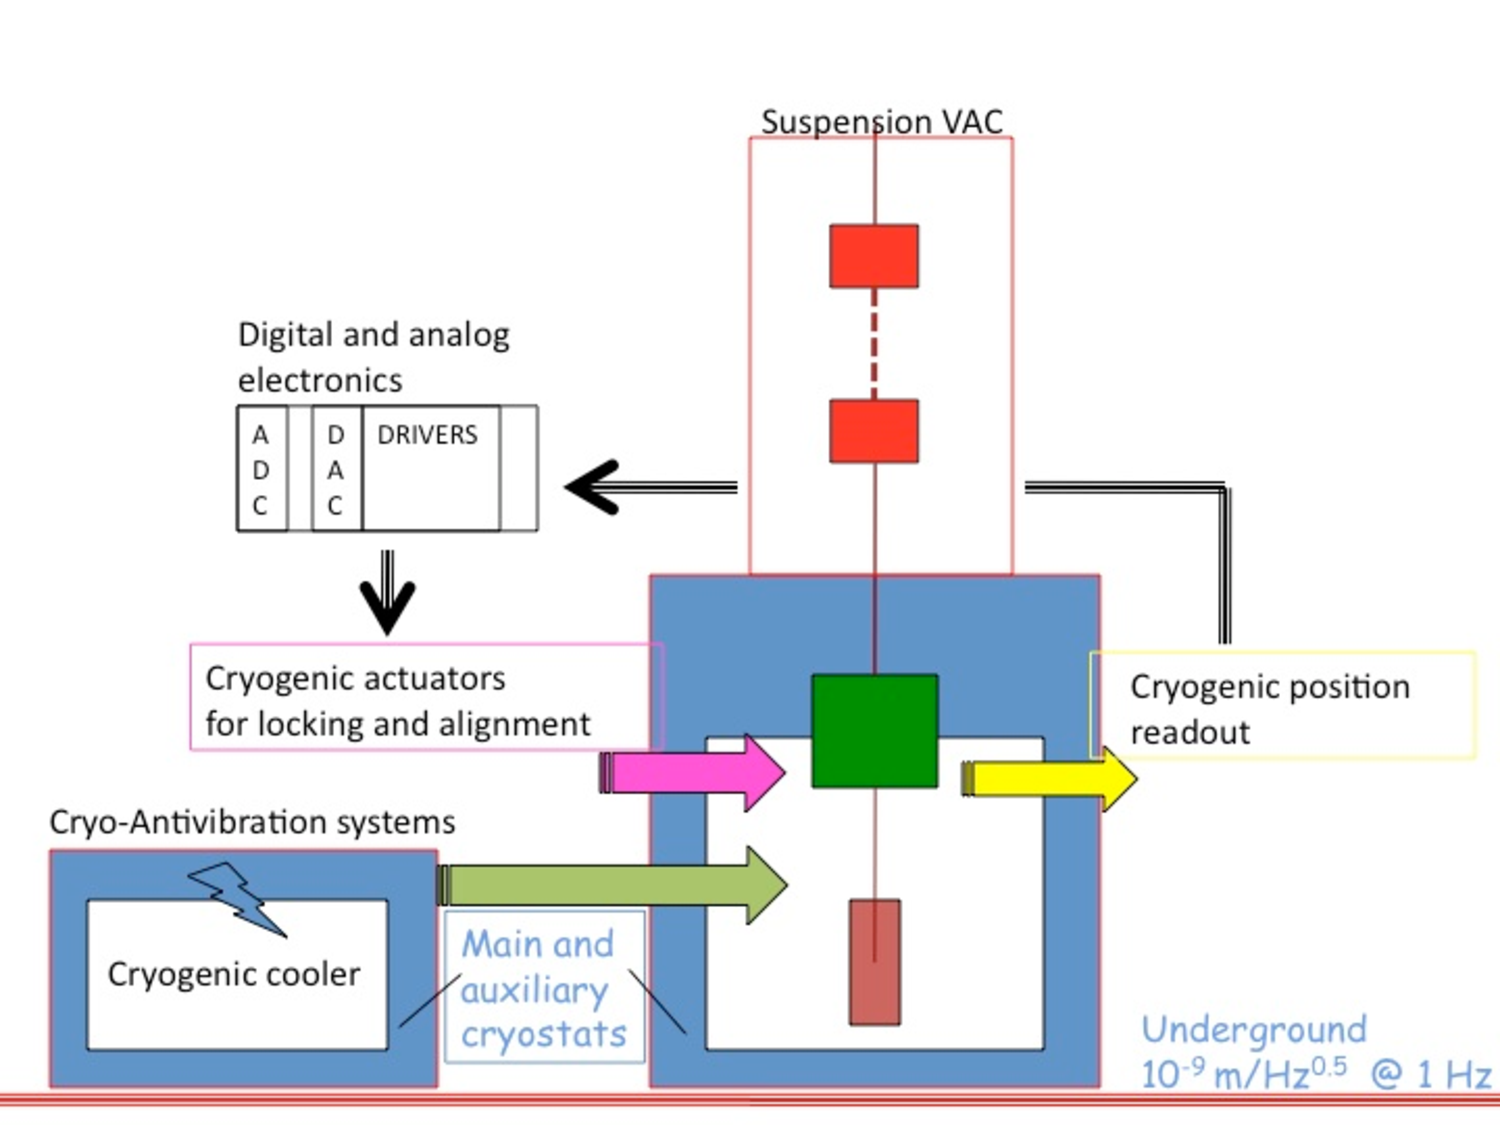
\includegraphics[width=0.6\textwidth]{Sec_Suspensions/Figures/overall.pdf}
\caption{\label{overall}\sf Schematic picture of ET suspension assembly concerning local control role. }
\label{fig:overall}
\end{center}
\end{figure}

The main issues that drive ET-related  R\&Ds concerning local controls leading to the identification of final solutions are listed below. 
\begin{itemize}
\item Sensing access to the mirror position without significant perturbation of cryostat performance in mirror cooling. 
\item Non-perturbing or reliably reproducible effect of cryogenics onto mirror position-sensing apparatus.
\item Compliance with  cryostat links and its vibration control system. 
\end{itemize}

For a cryogenic detector the viewports are sources of thermal input, a safe engineering approach is to limit the number of viewports to be installed. 
 
\noindent
The fibre-optic lever technique is the simplest method for non-contact and high-precision displacement detection. Its principle was originally recognised by Frank and Kissinger, then analysed by Cook and Hamm. The sensor utilises the internal reflection properties of step-index fibres that have significant motion sensitivity as a displacement transducer.       

\begin{figure}[h]
\begin{center}
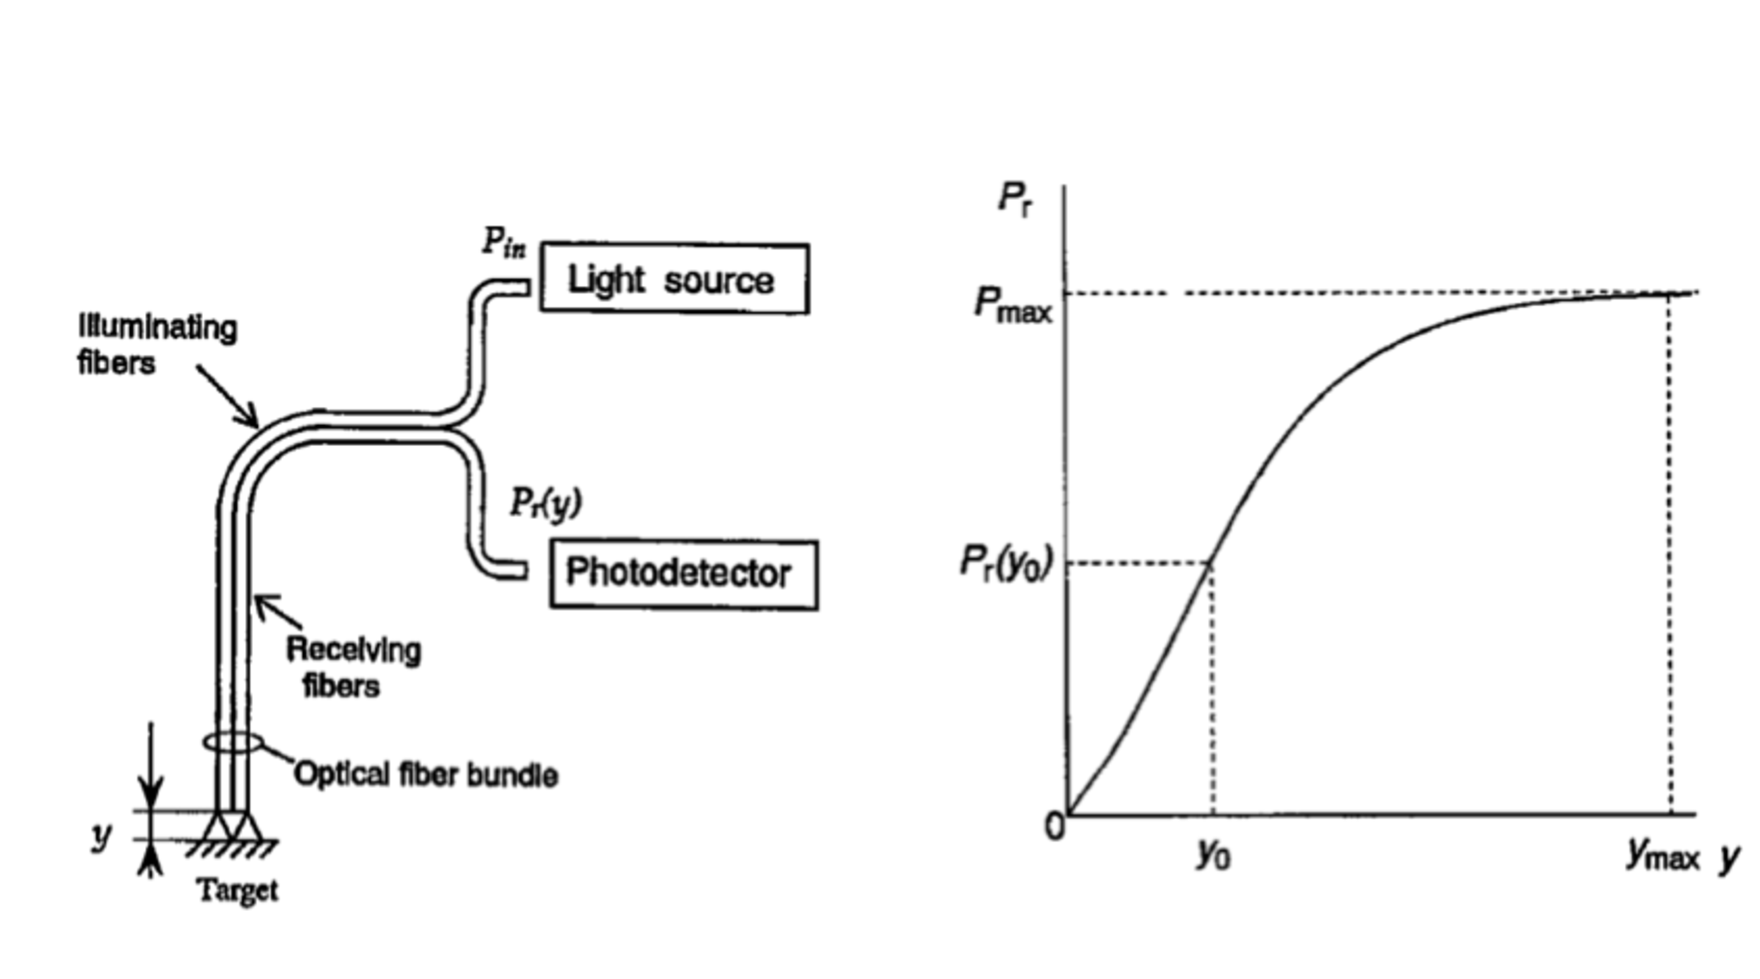
\includegraphics[width=10cm]{Sec_Suspensions/Figures/Fiber_tot.pdf}
\caption{On the left sensor we show a schematic illustration of a basic optical fibre displacement. On the right we plot a typical curve of the receiving light power versus the gap $y$ between the fibre bundle end and the target surface.}
\label{fig:fiber_bundle}
\end{center}
\end{figure}

\noindent 
The system consists of a light source, a bifurcated optical fibre bundle, and a photosensor. The light radiated from the light source enters the illuminating fibres and then radiates to a target. It forms a diverging cone or annular ring on the target surface. 
The reflected cone is differentially subtended as a function of the target distance, by receiving fibres 
and is transmitted to a photosensor. Consequently, the target distance is sensed by the photosensor as the subtended power. 
The device has been used successfully at low temperature during the cryogenic payload test carried on at the Virgo site.

To that extent, imaging systems (e.g.\ CMOS or CCD cameras), the use of optical conduits and bundle-fibre-served position sensor devices have also been considered for \emph{coarse} mirror control together with short-arm optical levers and small interferometric systems for \emph{fine} in order to provide the required dynamics of error signals (from several mrad's to nrad's).  The scheme of payload local control will be studied in compliance/integration with the spurious low-frequency vibration injection arising from cryogenic system. Hence low frequency cryogenic sensors (accelerometers) are being developed for this purpose.

Normally, as done in Virgo, the centres of mass of the suspension bodies are close to bending points of suspension wires. That is a condition which is particularly relevant for the marionette.  For ET the payload  will necessarily be controlled also transversally to the beam direction in order to prevent the mirror roll through the transmission of residual transversal disturbance reaching the marionette suspension point. Hence dedicated actuators and sensors will be added to the simple scheme of Virgo. In must be remarked that given the delicate balance demanded to payload  marionettes further balancing counterweights (transversal) will be also needed.

Even though the thermal contacts allowing the cooling down of the payload will transmit a vibration that can be made smaller than ground seismic vibration by using passive or active systems, from the point of view of the dynamical state of marionette's suspension point, isolated by the ground through the Superattenuator that will appear as a mechanical short-cut and expectedly dedicated inertial sensing/control system will be needed at the level of Superattenuator/payload interface.

\FloatBarrier
\subsubsection{The  coil--magnet actuators}
\label{sec:em_actuator}
%\emph{
%Author(s): F.\ Ricci, P.\ Falferi}

The actuators acting on the marionette and the reaction mass are designed to allow active control of the locking and alignment during operation.

Small and fast corrections of the mirror position can be obtained, through the marionette, if the mechanical transfer function of the system is taken into account. For example, due to the response of pendulum mechanical filters, the displacement amplitude of the mirror face with respect to that applied to the marionette arms decreases with the frequency. Then, in order to avoid self-oscillations at higher frequencies, a significant increase of the feedback gain, at the edge of the dynamics of the electronics, is needed. Furthermore, when forces are applied to the marionette, the spectral components of the feedback energy can be absorbed at the mechanical resonant frequencies of the SA, making the desired control more complex. Then, the need of direct actuation of the mirror for fast position control has motivated the use of a reaction mass.

In the present Virgo configuration two  magnets are placed on the marionette $x$ oriented arm and have the axis in the direction $z$. The other two, attached on the marionette $z$ arm, are oriented along $y$. Through these two pairs of actuators, and choosing properly the sign of the currents flowing into the coils, it is possible to steer, around $\theta_x$ and $\theta_y$ , and displace, along $y$ and $z$, the mirror and the reaction mass as a whole.
Longitudinal and angular forces can be applied to the mirror by coil-magnet actuators, which are attached to the reaction mass and the mirror respectively.

In order to design the coil - magnet actuators for the marionette and the mirror of the LF interferometer, several constraints must be taken into account.

Here we considered only the effect of the magnetic noise produced by the magnet at 4.2 K and its magnetisation change due to the cooling, the current noise of the coil and the power dissipated by the current flowing in the coil.

The force exerted onto the magnet by the coil is $F= \alpha \mu I$  where $\mu$ is the magnetic moment of the magnet, $I$ the current in the coil and $\alpha$ depends on geometrical factors. It can be shown that the interaction force has a maximum at an optimal distance between coil and magnet and can be considered constant for small displacements around this position and for small misalignment of the magnet axis with respect to that of the coil~\cite{LSSpaper1999}.
As $\mu$ and $I$ play the same role in determining the actuator force, similar considerations hold for both the quantities. 

As regards the magnetisation, measurements  have been carried out on a cylindrical SmCo magnet~\cite{MagneticShop}, 10\,mm diameter and  4\,mm height, axially magnetized, of the same type used in the Virgo marionette. The magnetic field at room temperature at the top surface of the magnet is 0.36\,T.
For convenience, all the low temperature data have been taken at 4.2\,K, in liquid helium at atmospheric pressure.
The measurements of magnetisation change have been performed with a fluxgate magnetometer with cryogenic probe and the magnetic noise measurements with a commercial SQUID system coupled to a superconducting pick-up coil fixed coaxially on the magnet~\ref{fig:SQUID_setup}. A detailed description of the experiment is reported in~\cite{Falferi_preparation} and here we summarise just the results having an impact on the ET design study. 

\begin{figure}[htbp]
\begin{center}
	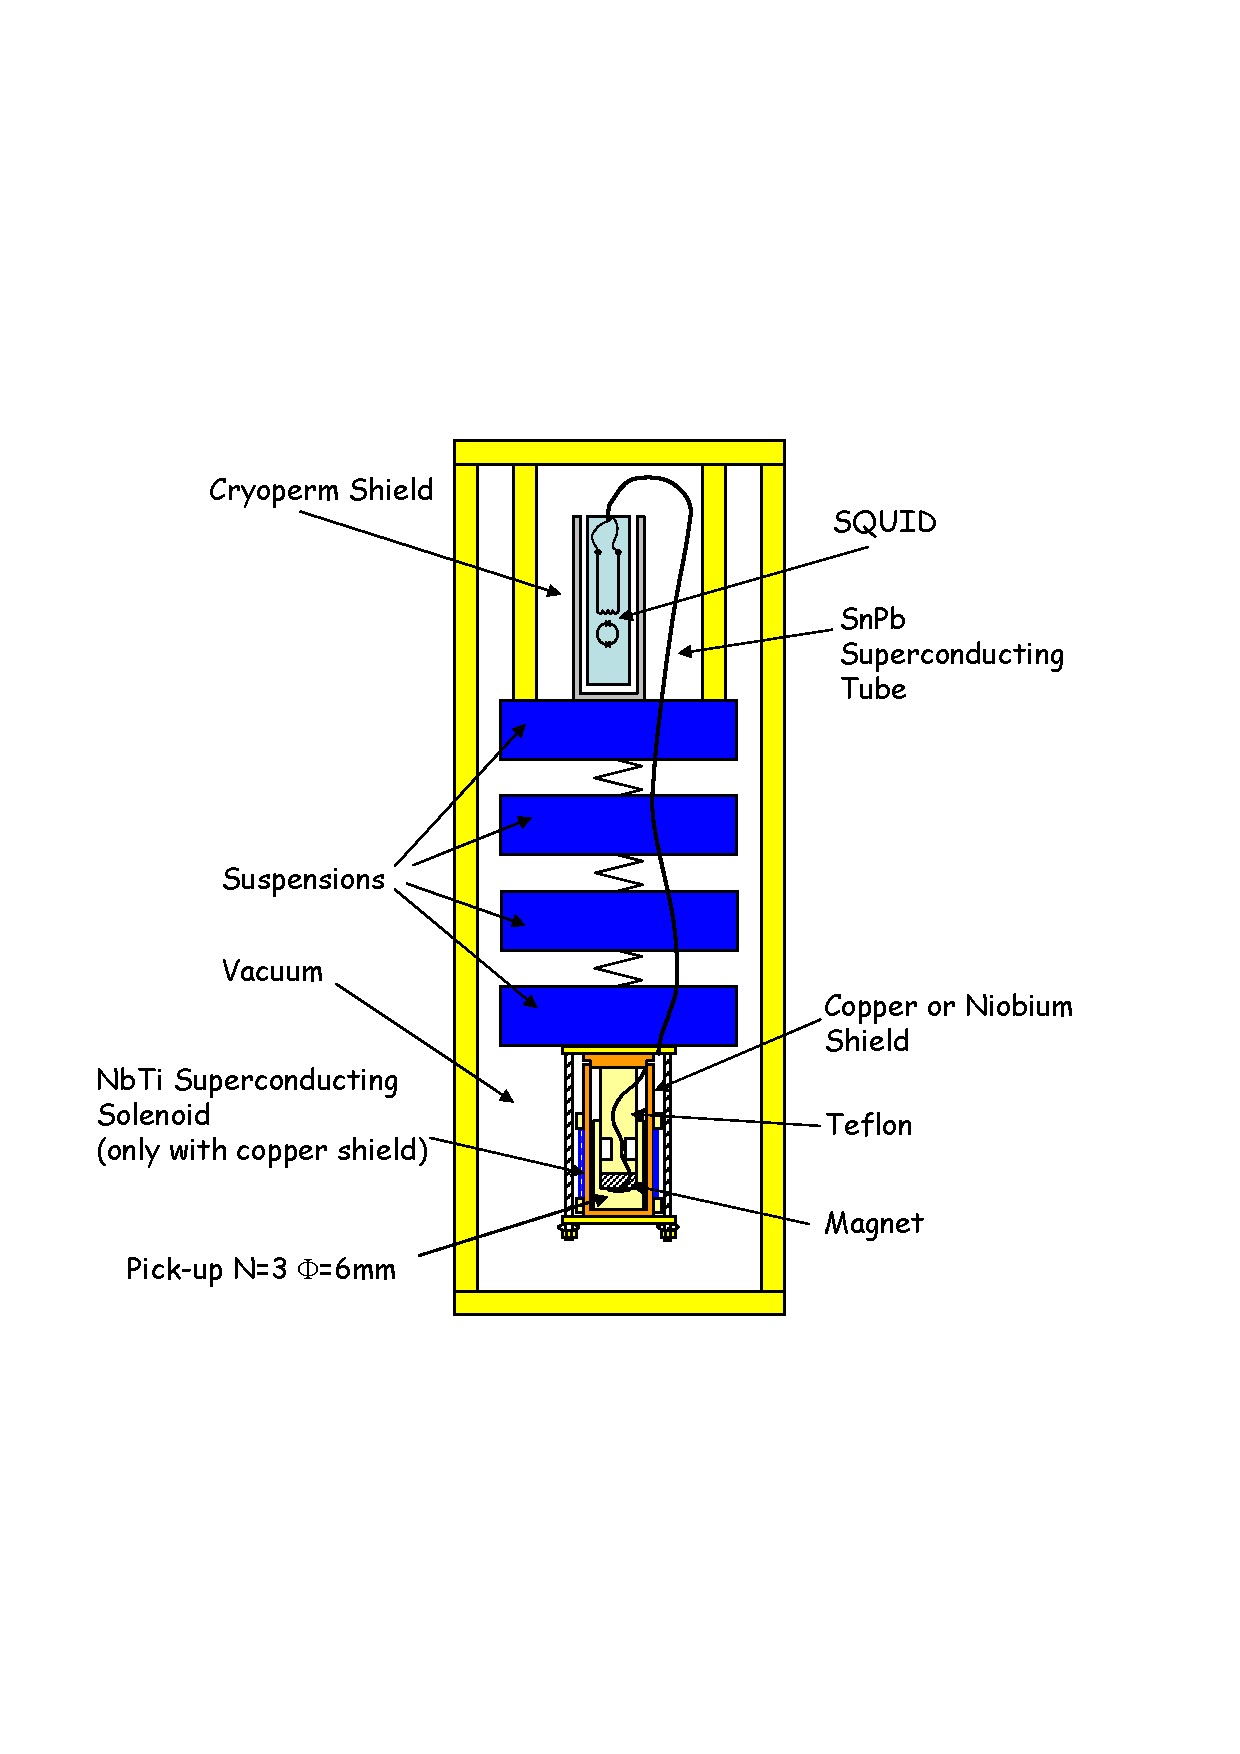
\includegraphics[height=90mm]{Sec_Suspensions/Figures/SQUID_setup.pdf}
	\caption{Experimental set for the magnetization noise measurements at 4.2\,K.}
	\label{fig:SQUID_setup}
\end{center}
\end{figure}


Figure~\ref{fig:SQUID_spectrum} shows a typical flux noise spectrum (calculated at the SQUID loop and expressed in units of  $\Phi_0 / \sqrt{Hz}$, $\Phi_0= 2.07 \times 10^{-15}$\,Wb), produced by the magnet in the niobium shield and obtained by combining two spectra taken with different frequency range and averages. 

In order to determine the different noise contributions, several noise measurements have been realised in different configurations.
The analysis of these measurements has suggested the following interpretation of the noise spectrum of figure~\ref{fig:SQUID_spectrum}.

\begin{figure}[htbp]
\begin{center}
	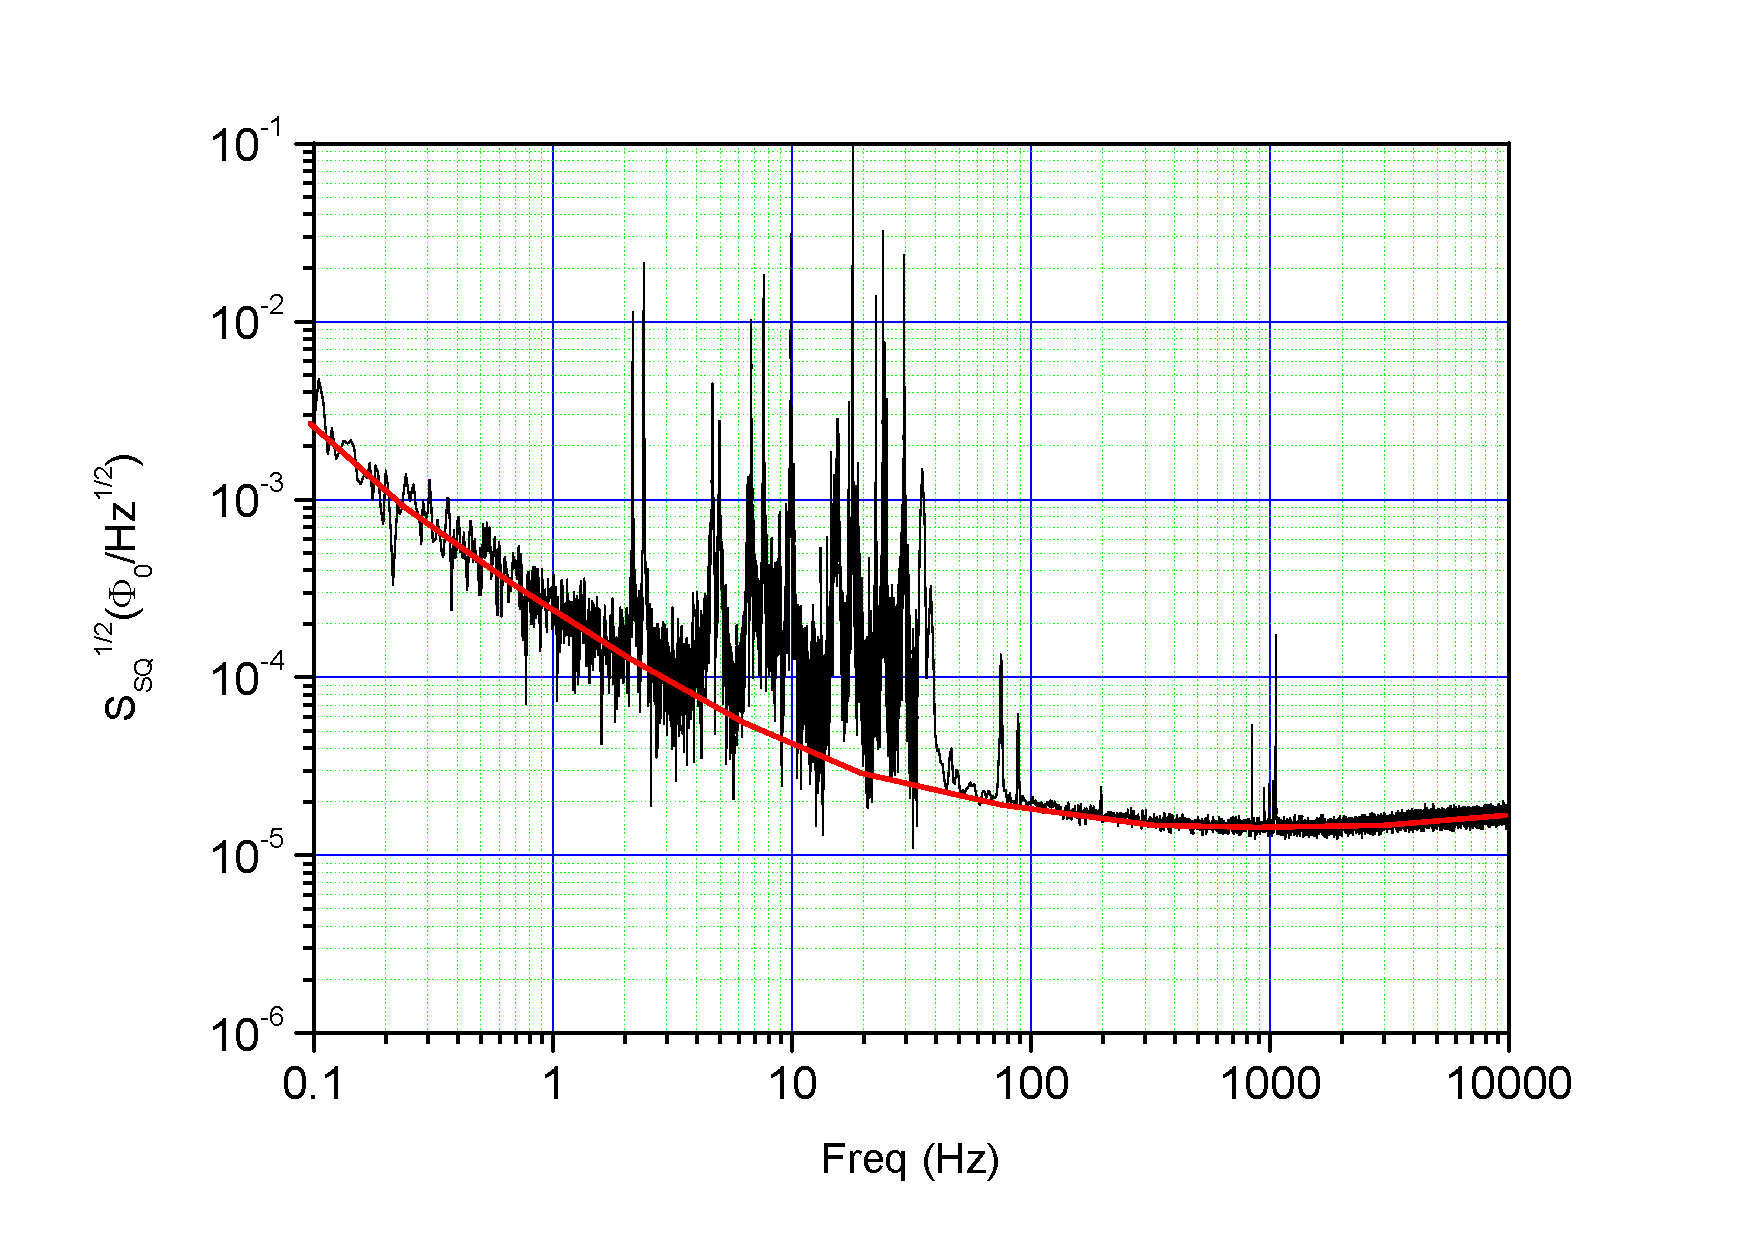
\includegraphics[width=80mm]{Sec_Suspensions/Figures/SQUID_spectrum.pdf}
\caption{The magnetic flux noise spectrum produced by the SmCo magnet and referred at the SQUID loop. The spectrum is obtained by combining two spectra taken with different frequency range and averages.}
\label{fig:SQUID_spectrum}
\end{center}
\end{figure}


At frequencies higher than 200-300 Hz the noise is dominated by thermal magnetic noise that is magnetic field fluctuations arising from the thermally agitated motion of electric charges of the conductor (SmCo in this case). This noise can be related to the temperature of the metal via a Nyquist type relation. A similar noise level has been obtained with the stainless steel cylinder.
Vibrational peaks are present between 2 e 100 Hz (as expected, suspensions are effective between 100 and 1000 Hz).
Between 0.1 and 4\,Hz the noise, of the $1/f$-type, is due to the magnet and tends to decrease with time.

We have also measured the noise produced by the magnet when it is subjected to a dc or low frequency (0.1\,Hz) magnetic field with magnitude comparable to that needed to produce a force of the order of 1 mN.  All the tests have shown that the application of magnetic field does not change the noise of the magnet.

The frequency range 2--100\,Hz is dominated by vibrational peaks but the shape of the magnet intrinsic noise can be easily guessed and is described by the red curve in figure~\ref{fig:SQUID_spectrum} that we consider as reference noise level for the following calculation of the force noise acting on the mirror. 

As the force of the actuator is proportional to the magnetic moment of the magnet and this is proportional to the magnetic flux picked-up by the pick-up coil connected to the SQUID, we have

\begin{equation}
\frac { {S_{\Phi p}}^ {1/2} } { \Phi_p } = \frac  {{S_{F}}^{1/2}} {F}	
\label{eq:Flux_1}
\end{equation}

\noindent
where ${{S_{\Phi p}}^ {1/2}}$ is the flux noise at the pick-up in $\mathrm{Wb/\sqrt{Hz}}$, $\Phi_p$ is the DC flux at the pick-up in Wb, ${S_F}^{1/2}$ is the maximum force noise of the actuator in $\mathrm{N/ \sqrt{Hz}}$ when the maximum force $F$ is generated.

Then, from the noise spectrum of figure~\ref{fig:SQUID_spectrum} expressed as the equivalent flux noise at the pick-up ${{S_{\Phi p}}^ {1/2}}$, the dc flux that crosses the pick-up $\Phi_p$, and the maximum force $F$ needed, the force noise that the actuator exerts on the mirror (or the marionette) can be estimated.

For example, considering one of the mirror actuators with a maximum force needed of 0.1\,mN and the mirror (200\,kg) as a free mass one can calculate, from the force noise, the displacement noise spectrum and then the equivalent strain noise spectrum on the basis of the 10\,km arm length ET-D LF model. The comparison with the ET-D LF total noise is shown in figure \ref{fig:actuator_magnetic_noise_contribution}.

\begin{figure}[htbp]
\begin{center}
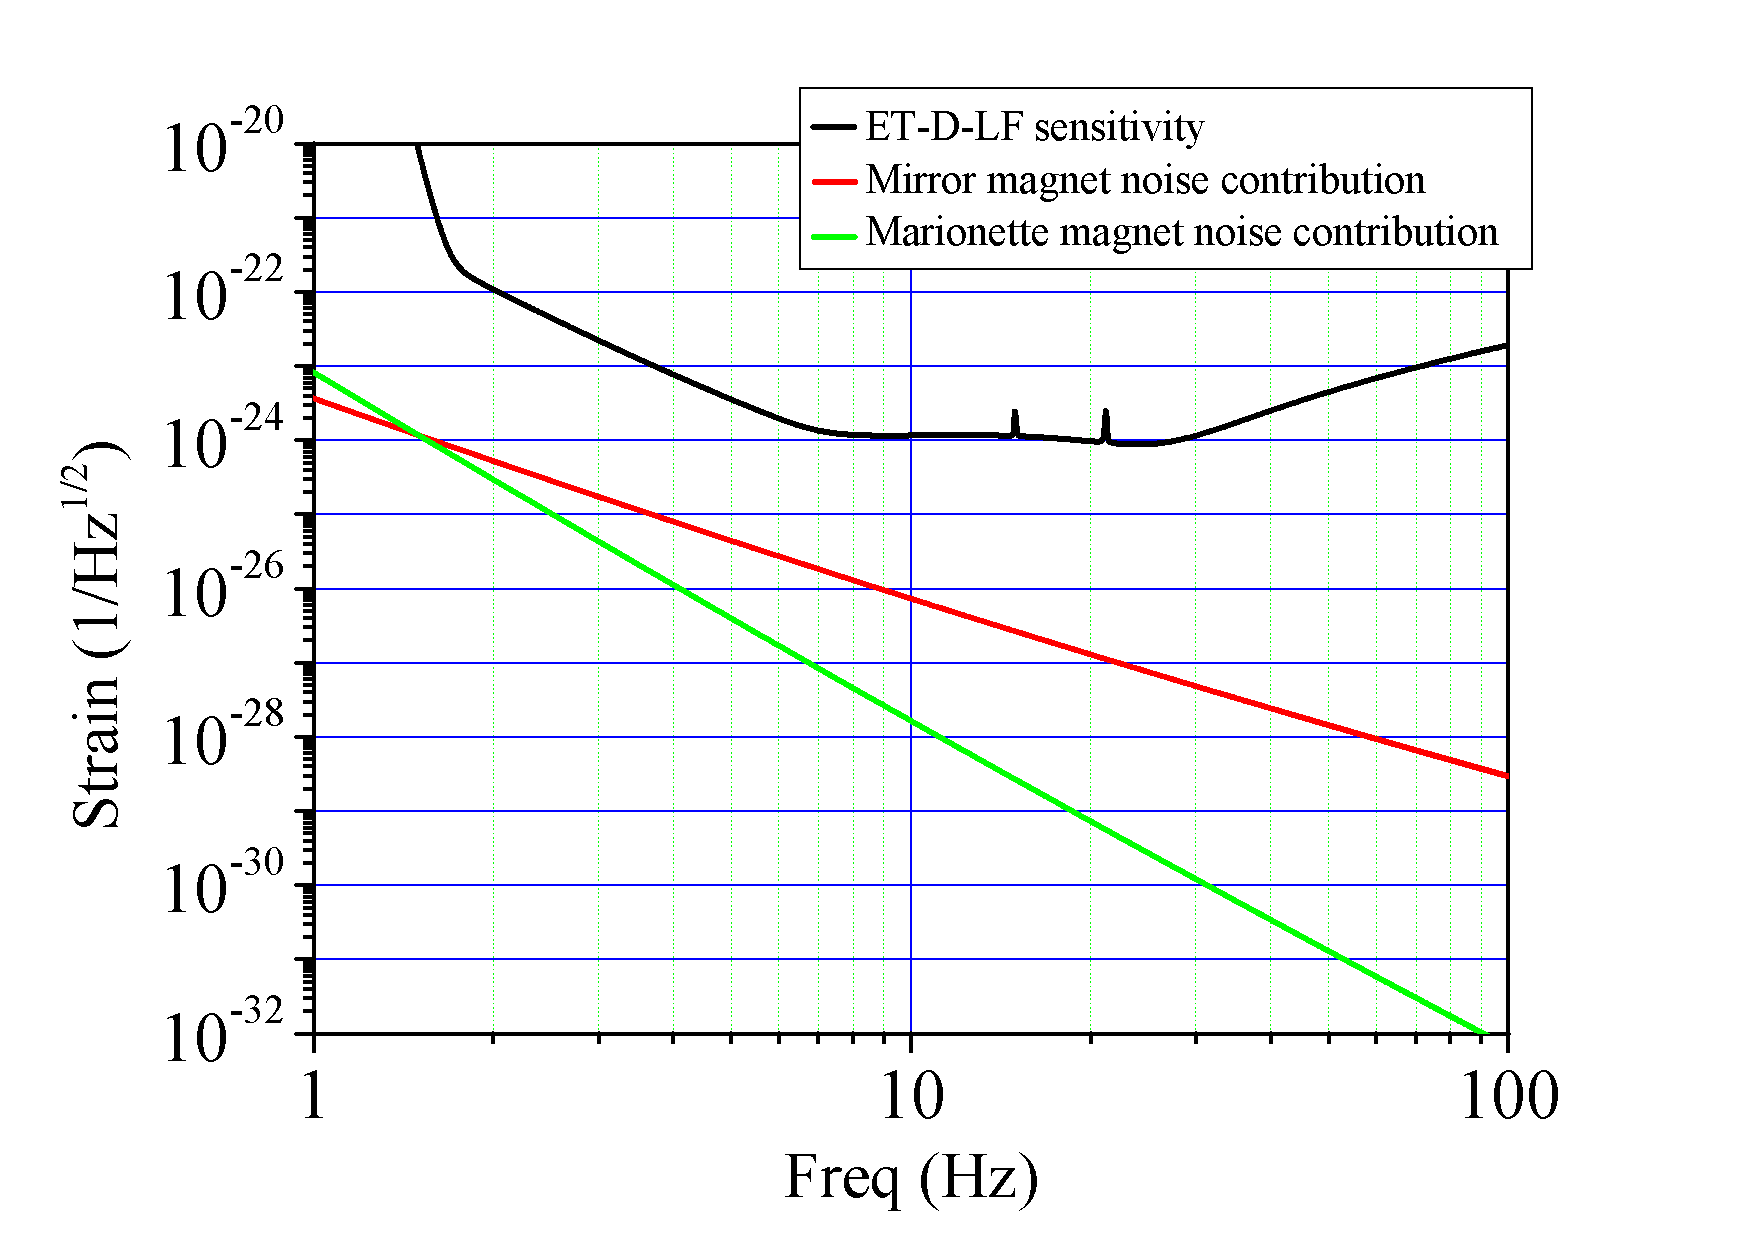
\includegraphics[width=10cm]{Sec_Suspensions/Figures/actuator_magnetic_noise_contribution.pdf}
\caption{Magnetic noise contribution to the strain sensitivity in the case of maximum force of 0.1 and 0.5\,mN  compared to the ET D sensitivity curve.}
\label{fig:actuator_magnetic_noise_contribution}
\end{center}
\end{figure}

In the same figure it is also shown the strain noise contribution considering one of the marionette actuators with a maximum force needed of 5\,mN. This rough estimation has been obtained by assuming the marionette as a free mass and the resonance frequency of the mirror pendulum (about 0.3\,Hz) much less than the considered noise frequencies.

As is evident from this figure we can conclude that the displacement noise at the mirror level, induced by the coil-magnet actuators of the marionette and mirror, is negligible.

To design the actuators acting directly on the mirror a further constraint, related to the thermal noise of the mirror pendulum mode, has to be considered. 
The random magnetic force exerted by the actuators has to be kept below the intrinsic noise limit of the system, i.e.\ the mirror thermal noise force
 ${S_f}_T $ :
\begin{equation}
{S_f}_T = 4 k_B T Re\Big[ Z (\omega) \Big] = 4 k_B  T \frac{ \Phi M {\omega_o}^2}{\omega} 
\label{eq:thermal_noise_force}
\end{equation}
where $Z ( \omega )$ is the mechanical impedance of the suspended mass and $\Phi$ is the loss angle of the mechanical system assumed to be frequency independent. Here, the second equality holds in the simplified case of a simple pendulum. 

The e.m.\ actuators are used in the digital control loop to keep the interferometer locked.  During the operation, these kinds of actuators have to adjust the mirror position along a 1\,$\mu$m range.
As the force acting on the mirror is a linear function of the current $I$ flowing in the coils, we have introduced the actuation factor $\alpha_m = F^{(m)} / I$.	The	control loop, which concerns these magnetic actuators, is conceived to compensate the fast changes in the mirror position and orientation. The quantised electronic noise of the digital feedback loop drives the random motion of the mirror. The noise spectral density of the current driving the reaction mass coils is intrinsically related to the noise injected into the control loop by the readout. The simplest readout scheme is a system of two components: a photodiode and a mixer. This second element is needed to demodulate the signal of the interferometer. To characterise the noise figure of the photodiode we can introduce the  parameter $D^2$  defined as 

\begin{equation}
 D^2= \frac {\langle i_d \rangle ^2} {{S_i}_n} 
 \label{eq:D}
 \end{equation}
 
where $\rangle i_d \rangle$ is the mean current flowing into the mixer which follows the photodiode readout and the current noise spectral density of the photodiode:
 \begin{equation}
 {{S_i}_n} = 4 e^2 D^2
\label{eq:current_noise}
\end{equation}
Using  the two previous equations (\ref{eq:thermal_noise_force}), (\ref{eq:current_noise}) and  imposing the inequality  $ 4 e^2 D^2  {\alpha_m}^2 \ll {S_f}_T  $, 
we get the  upper limit for the actuation factor
\begin{equation}
\alpha_m \ll \frac{1}{e~D}\sqrt{ k_B T M \frac{ {\omega_o}^2 \Phi}{\omega }  } 
\label{eq:alpha}
\end{equation}

\noindent
A typical figure of the ET parameters  is:
 $\Phi \sim  10^{-8}$, $M \sim 200$\,kg, $\omega_0/ 2 \pi \sim 0.3$\,Hz, $D\sim 10^8 \, \sqrt{\mathrm{Hz}}$, and $T \sim 10$\,K. Then, from equation~(\ref{eq:alpha}) we derive the upper limit at $\omega/2\pi \sim 1$\,Hz:

\begin{equation}
 {\alpha_m}^{(max)} \simeq 4 \times 10^{-4} \, \mathrm{N/A} 
 \label{eq:alpha_m}
 \end{equation}

The typical driving current of the actuators compatible with the low  noise regime of the electronic drivers is in the range of few mA. It follows that the maximum force exerted on the mirror will be in the range of 10 $\mu$N providing to use   magnets of  small magnetic moment  in order to limit the viscous dissipation effect due to the eddy currents on marionette and  reaction mass. However, in order to achieve the condition in which, at low frequency, the ET  sensitivity is limited by the internal friction of the mirror pendulum mode, we must use a dielectric material both for the reaction mass and the marionette arms.

\etbox{r}{box:Joule_dissipation}{The need of low dissipative actuators for ET-LF payload}{ 
We have to point out that in a cryogenic apparatus we need to limit  the  power dissipated in vacuum by  the current flowing into the actuator coil.  It useful to report here the observation done on a prototype of cryogenic payload cooled at 10\,K. The payload  has the typical dimensions of the Virgo and  it holds a fake 20\,kg mirror made of silicon.  It is equipped with actuator coils made of copper, by means of which we measured  the electro-mechanical transfer function of system at low temperature. To do that  we need to drive the actuators with   an electric  current of few mA. Despite of the significant decrease of the copper resistivity with temperature, the heat radiated  in vacuum  cause a large drift of the temperature of silicon mass as it is shown in figure~\ref{fig;cryo_payload_temp_drift}. These measurements  suggested us  to design the ET coils made  of NbTi with the core made of copper. In this way at cryogenic temperatures we  will take advantage of the superconducting transition of the metallic alloy. 
\begin{figure}[H]
\begin{center}
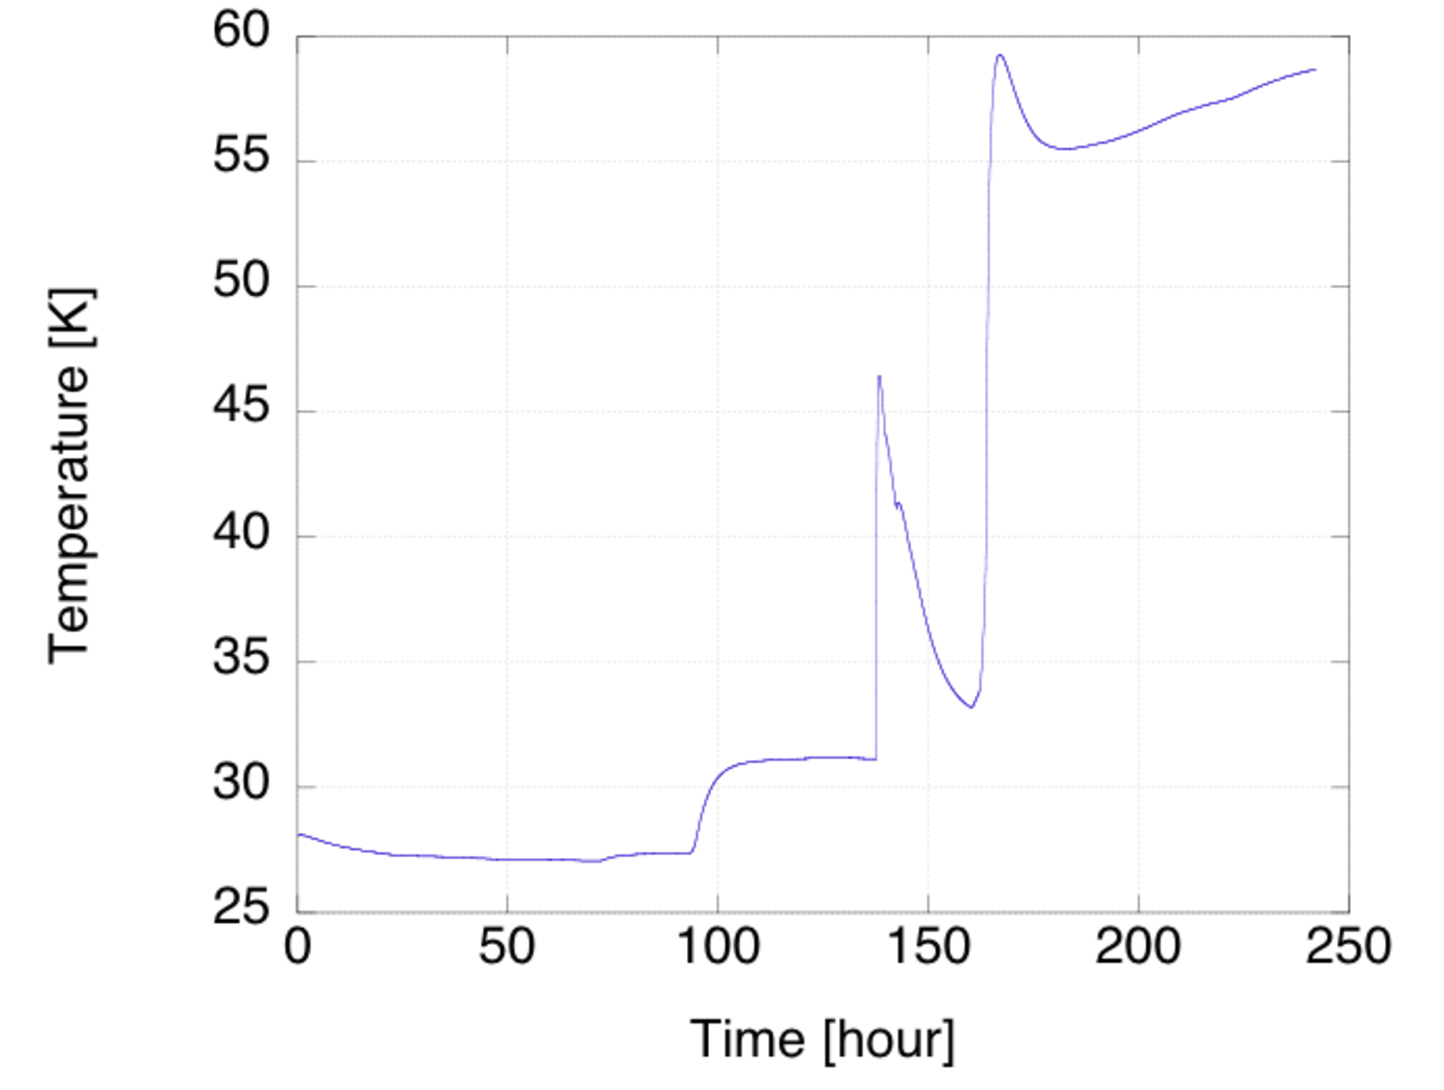
\includegraphics[width=7cm]{Sec_Suspensions/Figures/temperature_drift.pdf}
\caption{The temperature drift of the 20 kg silicon mirror hold in a prototype of cryogenic payload   during the mechanical transfer measurements.}
\label{fig;cryo_payload_temp_drift}
\end{center}
\end{figure}
}





\FloatBarrier
\subsubsection{The electrostatic actuators}
\label{sec:electrostatic}
%\emph{
%Author: R.\ De Rosa}


Electrostatic Actuators (EA) are an interesting alternative for the control of the test masses, respect to the widely used coil-magnet pairs.

Such solution was already applied for the GEO 600 detector~\cite{GeoCal} and it is under study also for other detectors, currently adopting coil-magnet pair actuators. The use of EA offers several advantages. The first one is the possibility to keep the mirrors under control without the need of gluing the magnets on the mirror bulk, saving, in this way, the mechanical quality of the test masses and, as a consequence, reducing the final thermal noise~\cite{Amico}. Another advantage is the strong reduction of the coupling with external magnetic fields, that is an important issue for magnetic actuators, since no direct coupling is anymore possible in the case of EA. Another possible advantage, mainly for third generation detectors, is linked to the possibility to control the suspended test mass, in science mode, only from the previous suspension stage, avoiding the need of a reference mass. In this case an electrostatic actuator, fixed on ground, represents the simplest way for the lock acquisition without adding any extra noise when the control is transferred to the upper stage.

The working principle of an electrostatic actuator is simply described by standard electrostatic, giving, for a device of capacitance $C$, polarized at fixed voltage $V$, a resulting force along the $x$ axis equal to:
\begin{equation}
\label{eqn:force_base}
F_x = - \frac{1}{2} \left| \frac{\mathrm{d} C}{\mathrm{d} x} \right| V^2=-\alpha V^2
\end{equation}
where the capacitance is supposed to vary by changing the system characteristics along the $x$ axis while the minus sign is due to the characteristic of such forces, that are always attractive.
In the case of actuator for suspended dielectric mirrors, such devices mainly consist in a set of close conductive strips, arranged in a suitable geometry, alternately polarised at two different voltages.
The strips, together with the dielectric suspended test mass, placed at distance a $x$ with respect to the actuator plane, constitute a capacitor, with a capacitance variable by changing the distance of the test mass with respect to the actuator.

The deduction of the theoretical expression of the capacitance, for such system, is described in \cite{Grasso}. It can be written as:
For the simplest geometry, i.e.\ a set of $N$ parallel conductive strips with period $b$, rectangular in shape, of length $L$ and width $a$, laying on a substrate with relative dielectric constant $\epsilon_{s}$, placed at distance $x$ from the test mass having a relative dielectric constant $\epsilon_{m}$, the capacitance can be written as:
\begin{equation}
\label{eqn:c_exp}
C(x)=C_\infty \alpha_m\left(\tilde{a},\tilde{x},\epsilon_m\right)
\end{equation}
where $\tilde{a}=a/b$ is the normalised strip width, $\tilde{x}=x/b$ is the normalised distance, $\alpha_m$ is a function of the listed parameters describing the effect of the mirror at distance $x$, and $C_\infty$ is the capacitance of the isolated actuator (i.e.\ with $x\rightarrow+\infty$).
This expression is calculated in the approximation of infinitely long strips and taking into account only the contribution of the first image charges, both for the substrate and for the mirror. As a consequence the capacitance of real devices become different from the this value for small values of $x$ with respect to $b$ due to the increasing weight of border effects and image charges as the distance decreases \cite{Grasso}. 

The force expression (\ref{eqn:force_base}) has to be modified to consider also the presence of a stray electric charge $q$ on the dielectric mass. In this case, by making the simple approximation that the electric field is proportional to the polarisation voltage applied to the actuator, it is possible to write:
\begin{equation}
\label{eqn:total_force}
F_x = -\alpha V^2 +\beta V
\end{equation}
where the factor $\beta$ is, in general, a function of the charge $q$, the distance $x$ and the geometry of the actuator.
The effects of this term were already observed on a similar set-up \cite{Mortonson}, and some techniques for its mitigation were already developed \cite{GeoCharge}. To reduce the effect of the stray charges, it is also possible to modulate the driving signal, to obtain a zero averaged contribution of the linear term of the  actuation force even in presence of charges on the test masses \cite{ElDrive}. This driving technique was already successfully experimented in the control of a bench top Michelson interferometer with a suspended mirror controlled by a such EA \cite{ElAct}.

To clarify this approach, let $A(t)$ be the driving signal we want to apply on the test mass, $A_{DC}$ the voltage bias and $f_M=\omega_M/2\pi$ the modulation frequency of the full driving signal. The square root is computed and sent, with the modulation, to the actuator driver. In this way the voltage applied to the actuator is:
\begin{equation}
\label{eqn:voltage}
V=G\sqrt{A_{DC}+A(t)}\cos{\omega_M t}
\end{equation}
where $G$ is the gain of the EA driver. With this voltage, the force exerted on the test mass becomes:
\begin{equation}
\label{eqn:elac_force}
F=-\frac{1}{2}\alpha G^2\left( A_{DC}+A(t)\right)\left(1+\cos{2\omega_M t}\right)+\beta G \sqrt{A_{DC}+A(t)}\cos{\omega_M t}
\end{equation}
If the modulation frequency is chosen at enough high frequency to have negligible effects on the test mass motion and the frequency content of the driving signal is much smaller with respect to $f_M$, the main contribution of the force (\ref{eqn:elac_force}) only consists of a DC bias term plus a term proportional to the driving signal $A(t)$. This is the required behaviour for such actuator.

The characterization of an EA with such driving technique is described in \cite{ElDrive}.
\begin{figure}
\begin{minipage}{0.47\textwidth}
\begin{center}
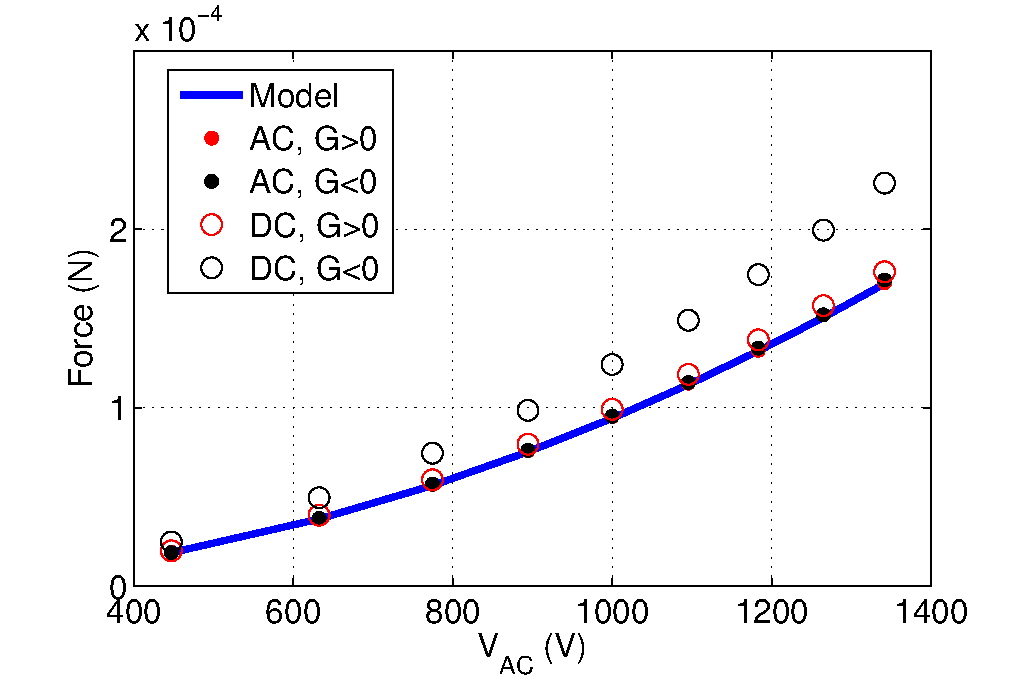
\includegraphics[width=\textwidth]{Sec_Suspensions/Figures/Measure1.pdf}   
\caption{\label{fig:measure1} Comparison between the model and the force measured, in different bias conditions, for a excitation with $f=0.1$\,Hz.}
\end{center}
\end{minipage}
\hspace{0.5cm}
\begin{minipage}{0.47\textwidth}
\begin{center}
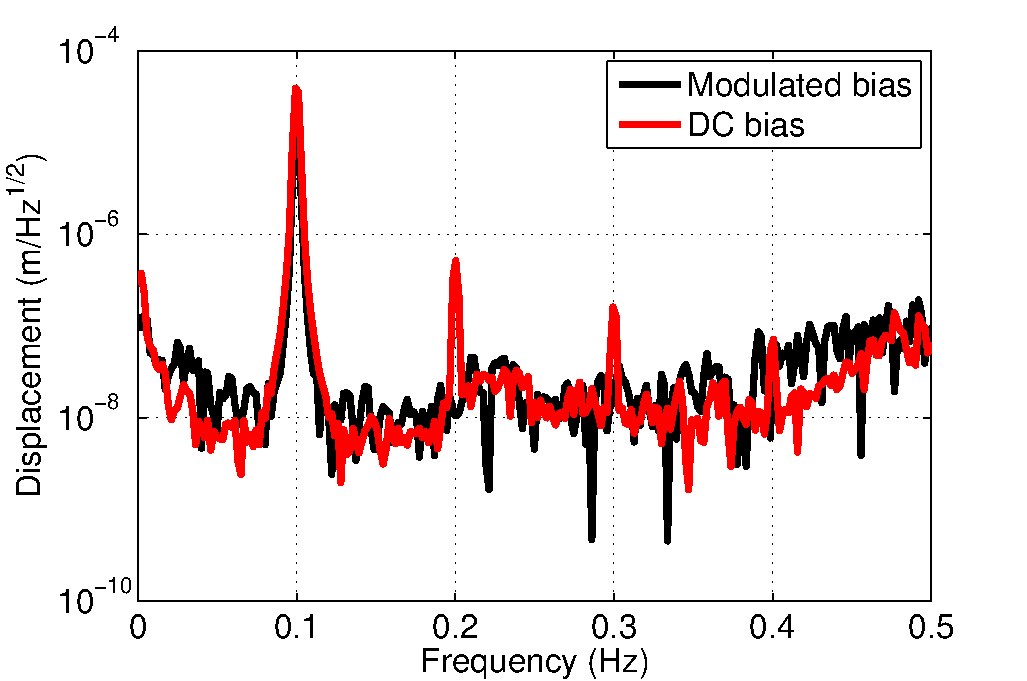
\includegraphics[width=\textwidth]{Sec_Suspensions/Figures/Charge.pdf}
\caption{\label{fig:charge} Spectra of the test mass displacement with the same actuation force, at $f=0.1$\,Hz in two different bias conditions.}
\end{center}
\end{minipage}
\end{figure}
The most interesting results are related to some observed deviation from the theoretical model. The measurements are shown in figure~\ref{fig:measure1}. The filled dots represent the force measured in AC bias, both with positive or negative $G$, while the open circles are the force measured in DC bias with different sign of $G$. The deviation from the foreseen behaviour, clearly visible for all the points in DC bias, in particular in the case of negative $G$, is due to the presence of spurious charges on the dielectric suspended mass. In fact in this case, equation (\ref{eqn:elac_force}) becomes:
\begin{equation}
\label{eqn:dc_force}
F=-\alpha G^2\left( A_{DC}+A_{AC}\cos{\omega t}\right)+\beta G \sqrt{A_{DC}+A_{AC}\cos{\omega t}}
\end{equation}
and a not negligible contribution could arise from the last term. Moreover this contribution depends on $G$ as confirmed by the results. The two opposite polarisation, for the AC bias, give instead the same results, as the experimental measurements are practically overlapped. This confirms the effectiveness of the alternate bias technique that is insensitive to any static stray charge present on the test mass.

Following the (\ref{eqn:dc_force}) a larger disagreement would be expected also for the case of DC bias with positive $G$, but  one should consider that the description of the electrical field between the EA and the test mass is very roughly approximated in the model; moreover a slight dependence of $\beta$ from the sing of $G$ is expected. More investigations are need in this direction which also require some upgrade in the experimental set-up, as the possibility to change the distance between the EA and the test mass without opening the chamber and changing, in this way, the amount of charges on the mass.
The displacement spectra, in case of measurements in DC bias conditions, also show additional lines placed at multiple frequency respect to the one injected by the signal. These lines disappear if the measurement is performed in AC bias as shown in figure~\ref{fig:charge}.

Starting from theoretical model, and on the basis of the previous results, it not too difficult to effectively design the electrostatic actuation system for ET. By assuming a mirror mass of 200 Kg (it is slightly higher for LF-ET, but the difference is not very relevant), a wire length of the last stage of 2\,m and a conservative residual motion of the test mass  $x \sim10 \, \mu$m, the minimum force required for damping the mirror motion is:
\begin{equation}
F \sim m\omega_0^2 x = 250 \, \mu\textrm{N}
\end{equation}
Since the beam radius is about 9 cm and the mirror diameter is 45 cm (in the worst case) the maximum reasonable residual space useful for the EA is about 10 cm. Moreover the distance between the test mass and the actuator has to be at least 5 mm, in order to reduce the damping from the residual pressure, and this also fix the period of the electrodes strip, that has to be close to the mirror-actuator distance to enhance the field fringes.
From these figures it results that each actuator can be composed by 5 strips large 4 mm arranged in concentric arches. For such pattern the model provide $\alpha=1.8\cdot10^{-10}$ N/V$^2$. By using equation~(\ref{eqn:force_base}) it results that the required force, using 4 pattern, can be achieved with a maximum voltage of about 600\,V, that is a good value for voltage amplifiers with low electronic noise and large bandwidth.
After the lock acquisition the actuation noise can be easily reduced by reducing the voltage bias of the actuator, hence by reducing the noise of two order of magnitude. Of course, in case of full locking reallocation at the marionette level the electrostatic actuator can even be switched off and no actuation noise is introduced.


\FloatBarrier
\subsection{Technologies to be developed}
\label{sec:technologies}
%\emph{
%Author(s):  M.\ Lorenzini, S.\ Reid, R.\ Nawrodt
%}


\FloatBarrier
\subsubsection{R\&D on the production of high purity silicon crystal fibre for the LF interferometer}
\label{sec:crystal-production} 
%\emph{ Author(s):  M.\ Lorenzini,
%S.\ Reid}

In designing the ET low frequency
    cryogenic interferometer, fused silica  monolithic suspensions are no longer
    suitable, due to a broad dissipation peak in silica around 40 K which spoils its performances. Among the suggested materials,
    silicon is very promising due to its very low intrinsic
    mechanical loss~\cite{lam}~\cite{McGuigan1978} and thanks to
    the high thermal conductivity, suitable to remove the heat
    deposited into mirrors by the laser.

Suspension elements must therefore be realised starting from
pure silicon material. A study~\cite{articolofibresil} has been
carried out on crystalline silicon fibres grown starting from a
melt of pure silicon and
 using the $\mu$-pulling down technique, to investigate the possibility of employing this technique in the realisation of silicon suspension elements
  in a cryogenic interferometer. The interest in this
  technique is manyfold. Besides of mechanical applications,
  silicon is a very important material for many  technological fields,
  such as electronics, photovoltaic industry, and integrated photonics.
  Let see some aspects in more details. The photovoltaic industry for solar
   cell production is  a rapidly expanding market. Many efforts are spent
   worldwide in order to increase the efficiency of solar cells or to diminish
   the production costs. In both respects the production of silicon fibres
    can play an important role because new geometrical schemes can be tested
    and the silicon fibres are produced directly in a ready-to-use  shape,
    thus cutting the processing costs and loss of material.
Another important potential application of Silicon fibres is
for the transmission and processing of signals in integrated
photonic circuits. Silicon has important optoelectronic
properties, such as its high thermal conductivity, high optical
damage threshold, and low losses in a wide spectral range from
1.2 to 6.6 $\mu$m. Recently Stimulated Raman Scattering (SRS)
has been used to demonstrate Raman laser in integrated
wave-guides in the near infrared (NIR) or for image amplifiers
in the mid infrared (MWIR). The production of optical fibres
with a silicon core would be an important complement to this
emerging research field, but up to now silicon fibres have had
a limited success due to the low crystal quality of the fibres.
In fact a new production technique that has recently been
presented is not capable to produce single crystal silicon-core
fibres~\cite{toncelli1} and the presence of several domains and
interfaces increase the transmission losses of the optical
device. The availability of single-crystal Silicon fibres would
be a great advance in this field, too.


The method of production consists in placing the melt in a
vitreous carbon crucible, heated with a radio frequency
generator. A seed of crystalline silicon is then inserted in an
orifice at the bottom of the crucible and pulled downward. The
melt cools down in a controlled way passing through the nozzle
and a fibre is grown (figure~\ref{camerasilfib.pdf}). About 15
crystalline silicon fibres have been grown
 with thickness ranging from 0.3 to 3 mm and length up to 310 mm (figure~\ref{fibressilfib.pdf}). Produced fibres showed a good diameter regularity for most of
 their length, except for some abrupt change in thickness probably due to instabilities in the RF generator. The crystalline
  orientation was determined using the Laue X-ray diffraction method: as a result, the fibres were not single crystals, but
  are composed of several single crystal parts.


\begin{figure}[h]
\begin{center}
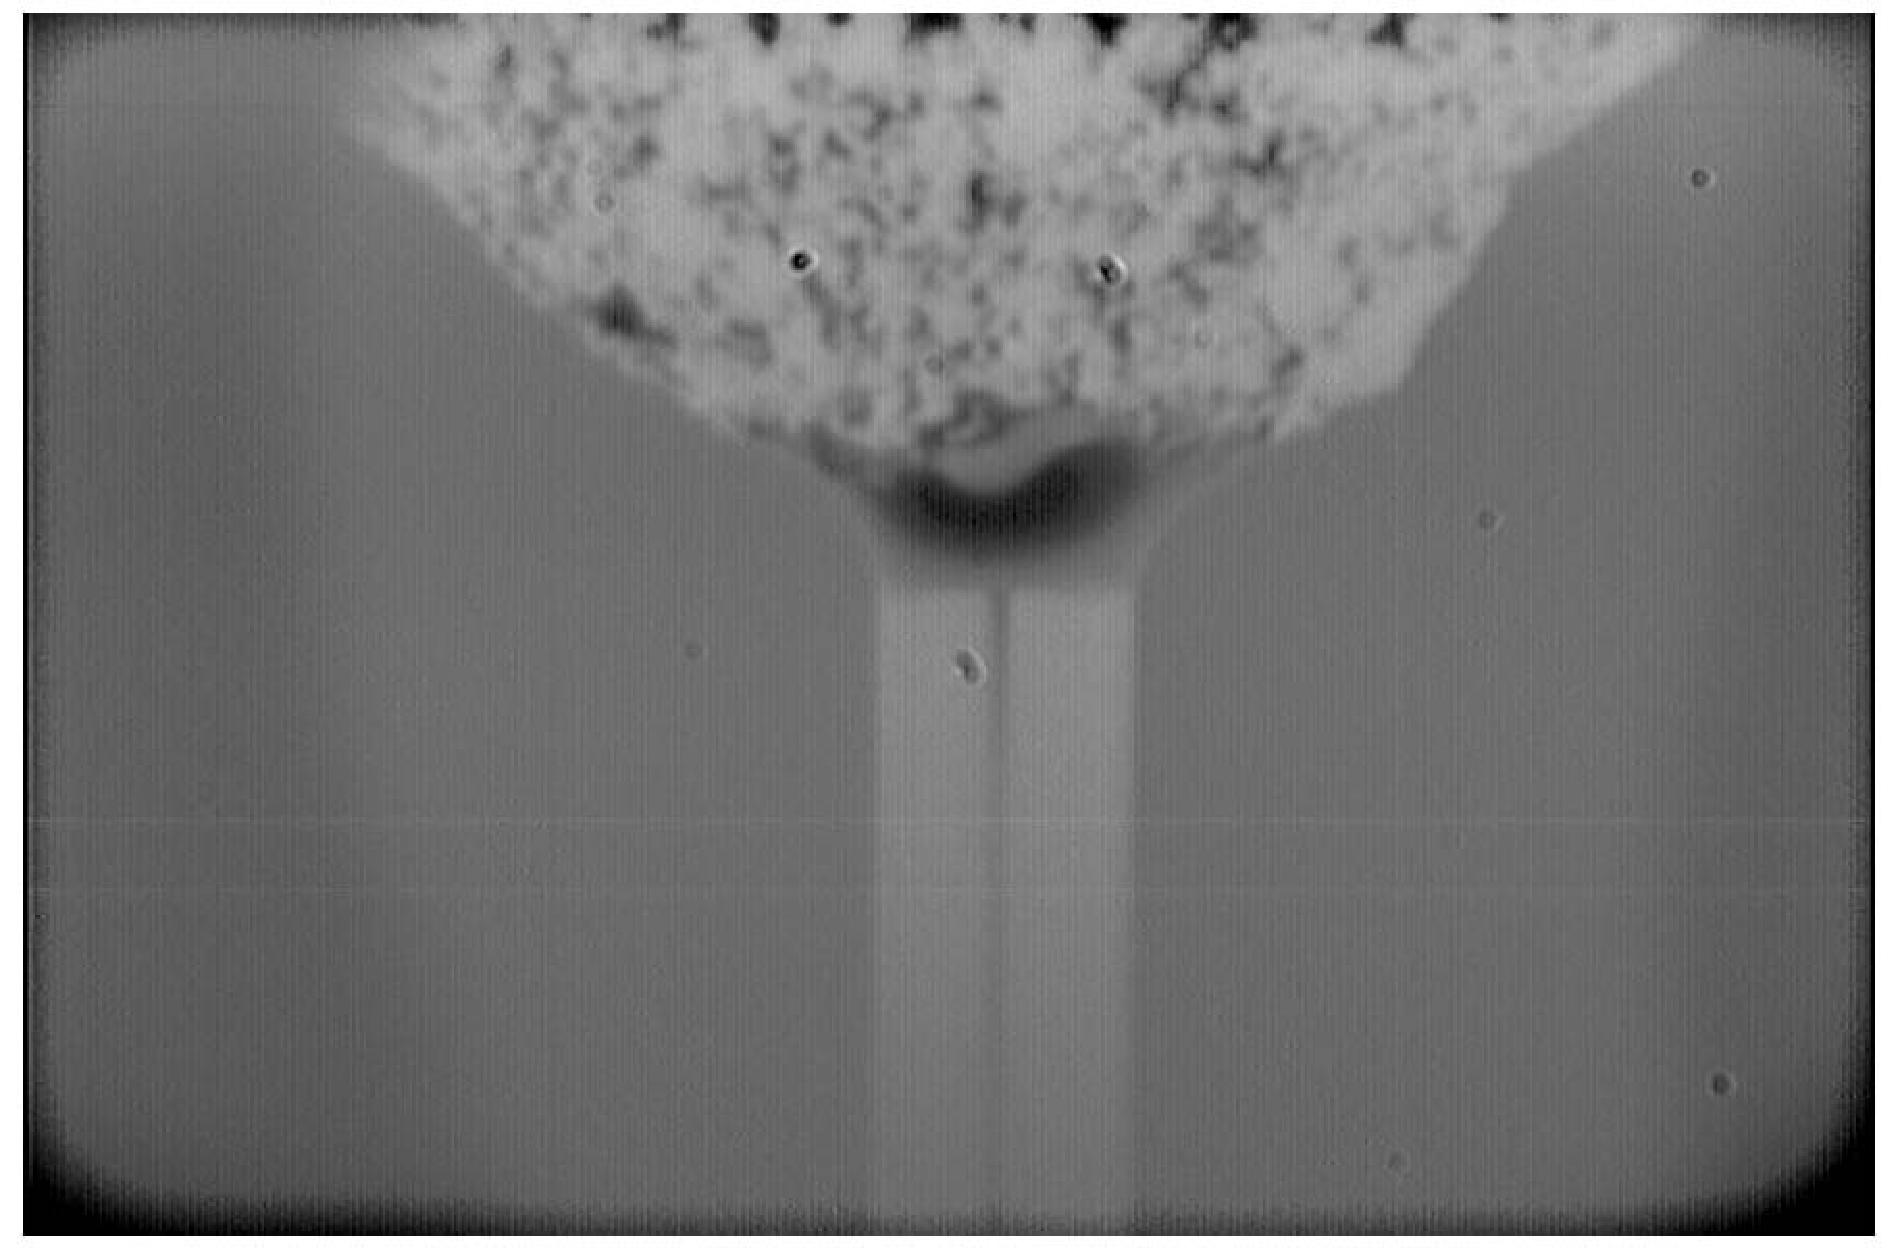
\includegraphics[width=20pc]{./Sec_Suspensions/Figures/camerasilfib.pdf}\hspace{2pc}%
\caption{A closeup view of the crucible nozzle during the production of a fibre.}\label{camerasilfib.pdf}
\end{center}
\end{figure}


 The loss angle of the fibres was evaluated at room temperature using a ring-down technique, and was dominated by the thermoelastic contribution.
 The thermoelastic loss peak allowed to experimentally measure the
 thermo-mechanical parameters of the realised fibres (see table~\ref{table1}). In order to get rid of surface
 contaminants (mainly SiC) the produced fibres were
 superficially etched before the measurements, using a HNA
 isotropic etching (in a 75\%HNO$_3$, 20\%HF, 5\%CH$_3$COOH
 solution).


\begin{figure}[h]
\begin{center}
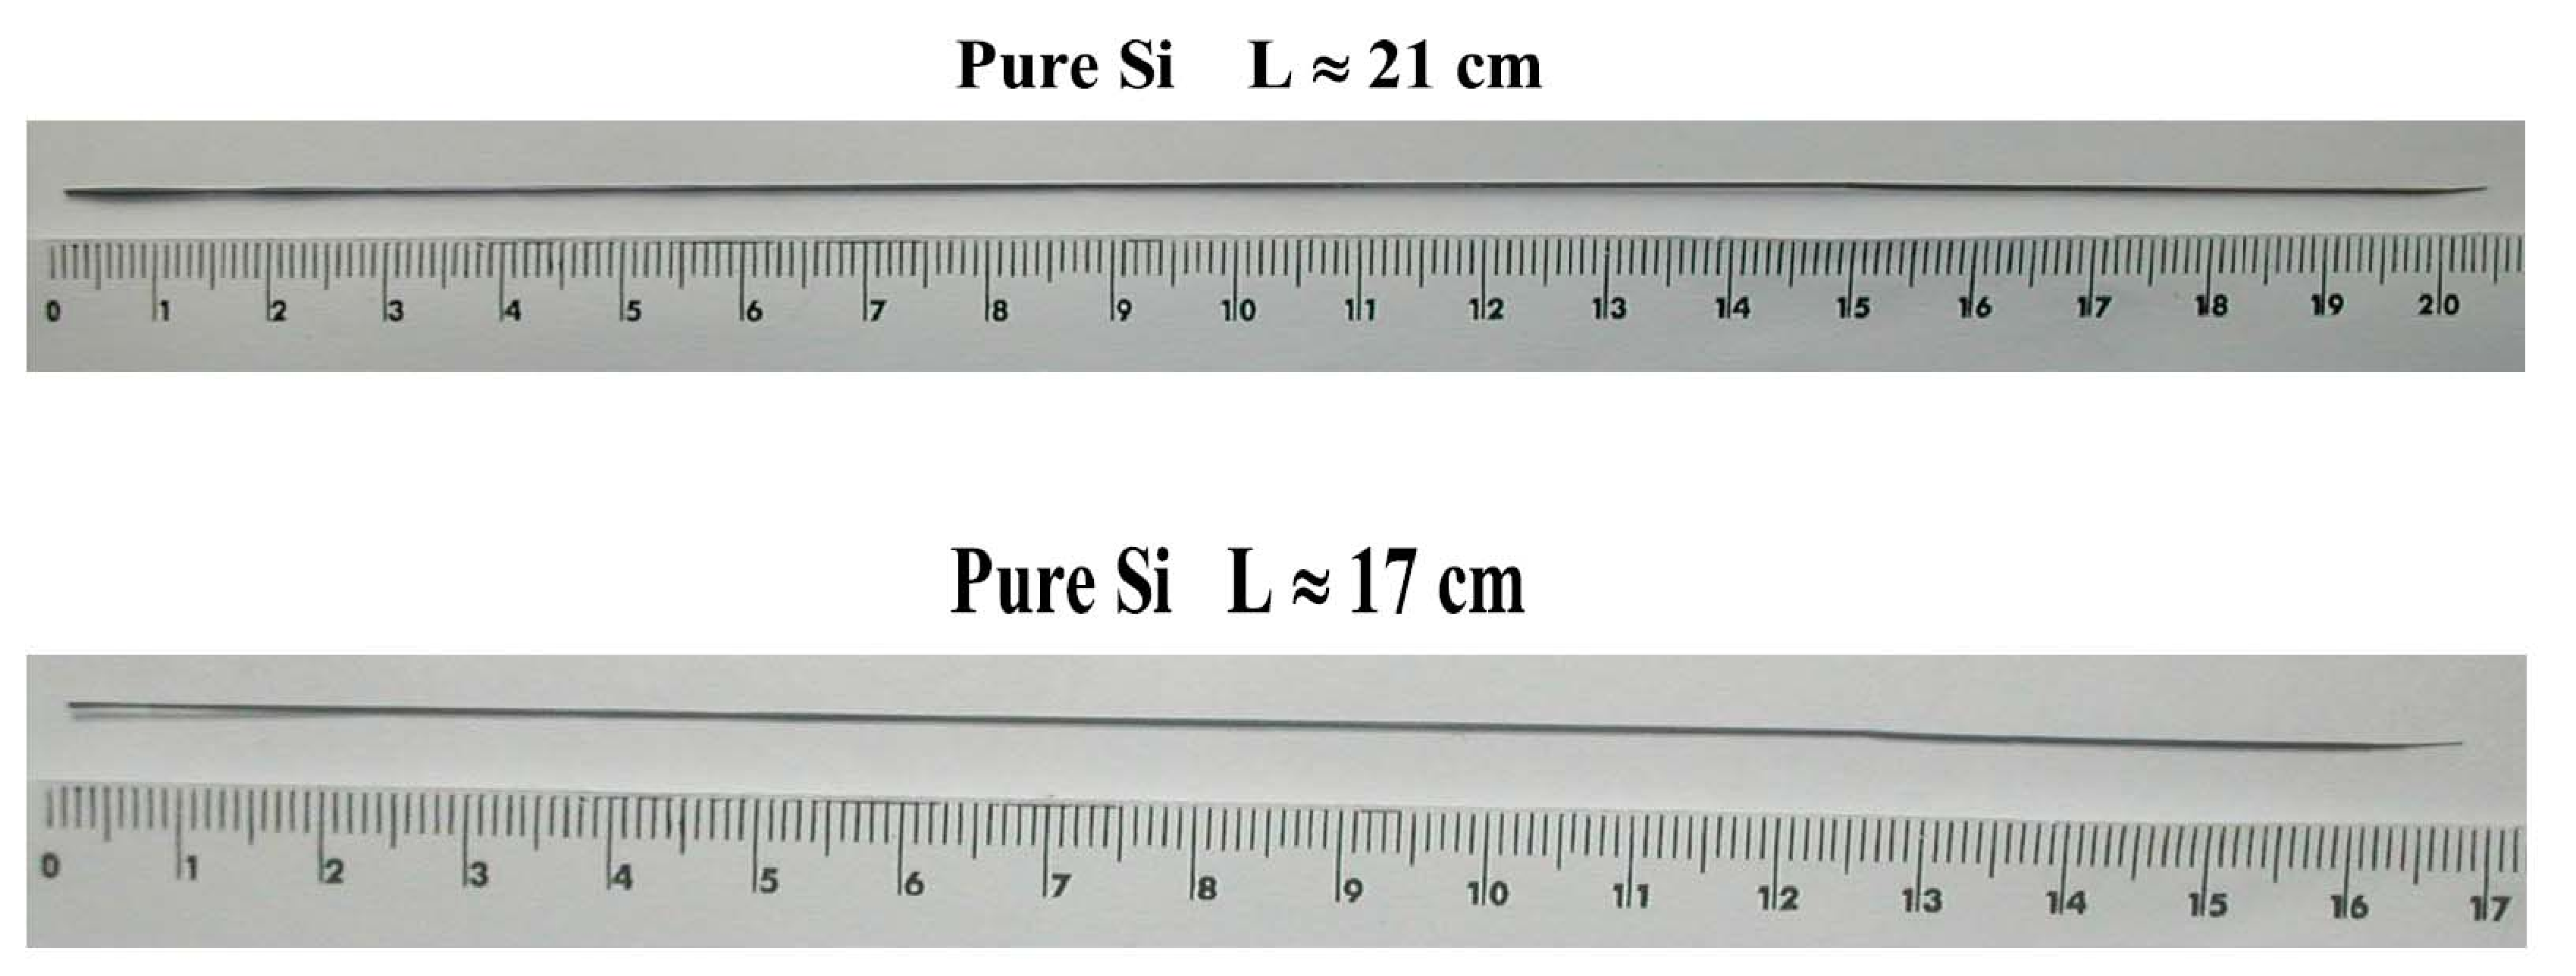
\includegraphics[width=28pc]{./Sec_Suspensions/Figures/fibressilfib.pdf}\hspace{2pc}%
\caption{Two silicon crystalline fibres produced using the $\mu$-pulling down technique.}\label{fibressilfib.pdf}
\end{center}
\end{figure}


The longest fibre among the produced ones was 310 mm long.
After this study, the technique has been improved and new
unpublished results have been obtained~\cite{toncellipers}.
They recently succeeded in growing single-crystal Silicon
fibres up to 10 cm long. In all cases the diameter is around 3
mm with small fluctuations (around 0.1 mm) along the whole
length of the fibre. A successive X-ray analysis confirmed the
single-crystal character of the fibres, and the only crystal
phase detected is that of pure Si. Moreover a SEM analysis did
not detect the presence of any impurity in the crystal material
within the sensitivity of the instrument. It is presumably
feasible to grow Si fibres with diameter from 0.5 mm up to 5-10
mm and virtually unlimited length. In the used facility the
maximum length possible is limited to 40 cm by the dimensions
of the pulling machine.


A problem was highlighted in the cited study, concerning the
welding of the produced fibres to other parts. Due to the very
high thermal conductivity, it turned out to be very hard to
weld the fibres tip to silicon pieces. The alternative to the
welding consists in using the parts to be welded as seeds for
the growth of the fibre. Similarly, the crucible can be removed
at the end of the pulling, leaving intact the contained
material: in this way, a fibre with a thick head can be
obtained. This procedure seems to be promising to realise a
monolithic silicon suspension and needs to be investigated
experimentally.



\begin{table}
\begin{center}
\end{center}
  \caption{Measured room temperature parameters for two crystalline Si fibres. Values are pretty close to the ones reported in literature for  silicon.}
  \label{table1}
  \begin{tabular}{cccc}
    \hline
    length [mm]& $E$ [GPa] & $\alpha$ [K$^{-1}$] & $\kappa$ [W m$^{-1}$ K$^{-1}$] \\
    \hline
    $111.5\pm0.5$ & $150\pm11$ & $(2.54\pm0.13)\times10^{-6}$ & $146\pm13$ \\
    $308.0\pm0.5$ & $174\pm12$ & $(2.56\pm0.11)\times10^{-6}$ & $138\pm11$ \\
    \hline
  \end{tabular}
\end{table}


This study proved the feasibility of thin silicon crystalline
fibres suitable to be employed as suspensions for a cryogenic
silicon mirror. The investigation of the loss and
thermomechanical behaviour of these fibres is an important step
in the technical development of the optimal suspension design.
More studies are needed to evaluate the fibres parameters in
cryogenic conditions.

\FloatBarrier
\subsubsection{R\&D on the bonding of silicon for the production of quasi-monolithic silicon suspensions}
\label{sec:bonding}
%\emph{
%Author: S.\ Reid
%}

%[perhaps necessary to plot thermal conductivity simulations for typical suspension geometries to above section?]

It will be necessary to identify the optimum method by which the silicon suspension elements may be attached to the silicon mirrors, whilst maintaining high thermal conductivity (for cryogenic operation) and low mechanical loss (to minimise thermal noise).  The technique of hydroxide-catalysis bonding [ref Gwo patent] was implemented in the GEO600 gravitational wave detector in order to create quasi-monolithic suspensions of the fused silica mirrors and is being used in the upgrades for Advanced LIGO and Advanced Virgo.  The resultant bonding material has been demonstrated to have very low mechanical losses [ref Sneddon, Smith, Cunningham] in addition to mechanical strength (shear) being reported being $>27$~MPa.  Studies also suggest that hydroxide catalysis bonding is unaffected by temperature cycling [ref Elliffe], which will also be crucial for the long-term operation of ET-LF, where the use of cryogenics is required to achieve the desired displacement sensitivity at low frequency.

Various studies have already been carried out to investigate the use of hydroxide catalysis bonding for jointing silicon components \cite{Veggel2009, Beveridge2011}.  This includes a detailed study of the mechanical strength of bonds at both room temperature and cryogenic temperature (77 K) \cite{Beveridge2011}, which is summarised in Figure~\ref{fig:silicon-bond-strengths}. The average bond strength at cryogenic temperature is similar to that at room temperature, albeit with a slightly larger dispersion. No correlation was observed between oxide layer thickness and bond strength above $\sim 50$~nm, therefore the oxide layer thickness should be minimised to this level to minimise potential thermal noise.

\begin{figure}[htbp]
\begin{center}
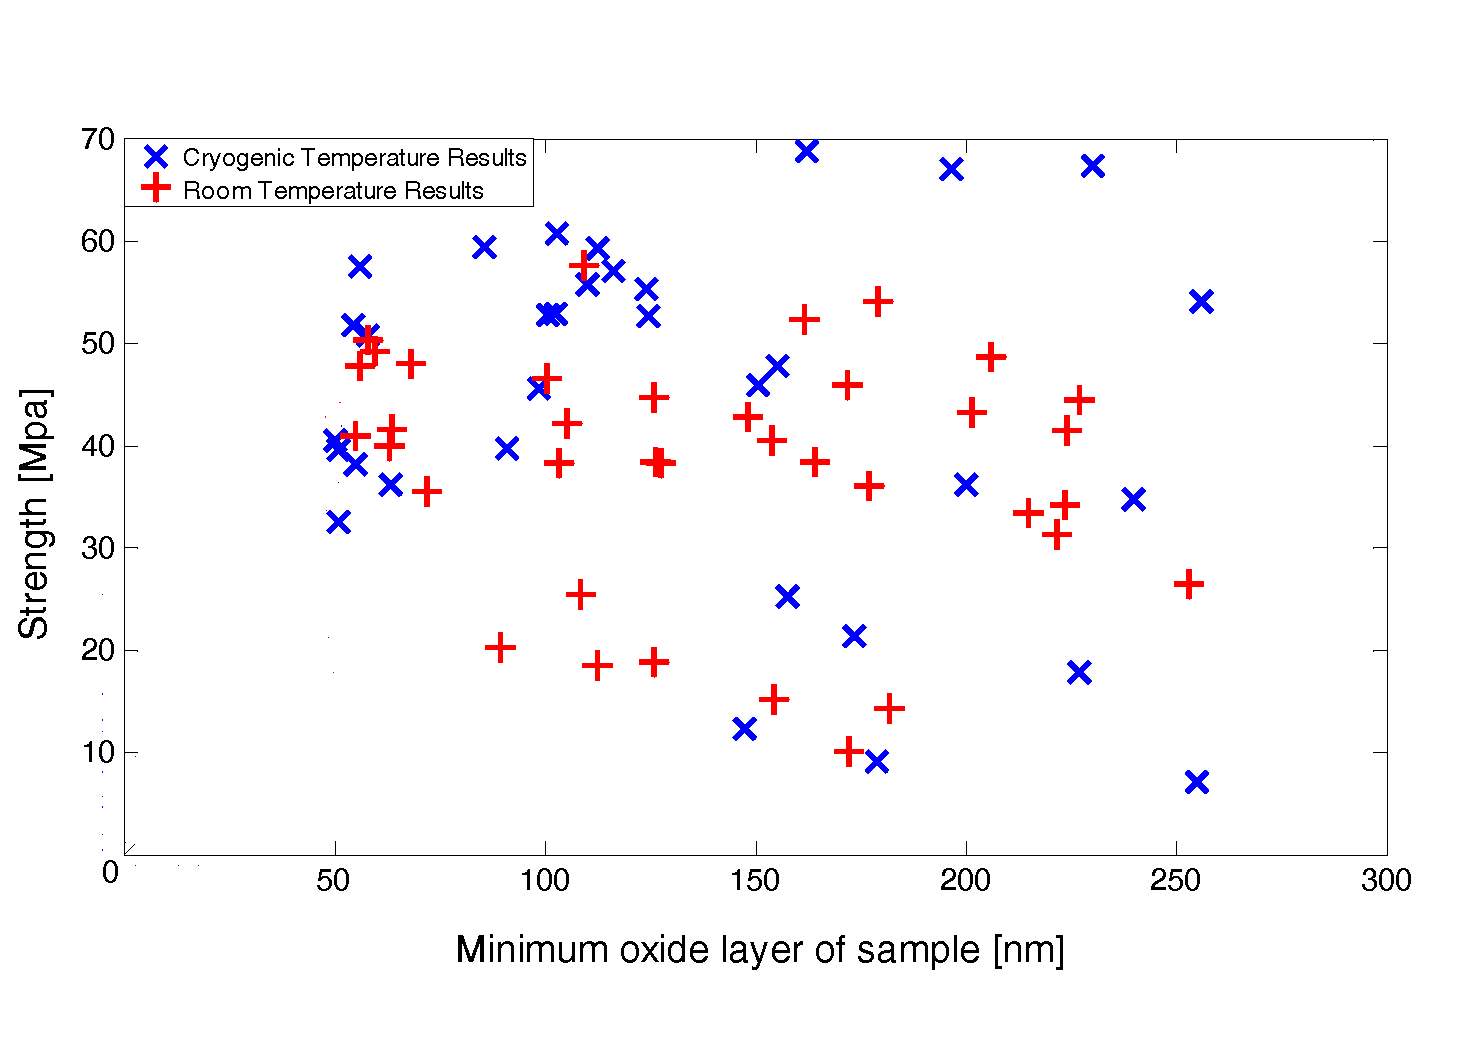
\includegraphics[width=100mm]{Sec_Suspensions/Figures/silicon-bond-strengths.pdf}
\caption{Plotted strength results for various silicon-silicon bonds at room and cryogenic (77 K) temperatures.}
\label{fig:silicon-bond-strengths}
\end{center}
\end{figure}

Studies are also ongoing into quantifying the thermal conductivity of bonded silicon components at low temperatures. Measurements of the thermal conductivity suggest that bonded silicon components at low temperature can be modelled as pure silicon with an thin ($\sim 700$ nm) interfacing glass-like layer. These results, as shown in Figure~\ref{fig:silicon-bond-thermal-conductivity}, suggest that hydroxide catalysis bonding can facilitate the necessary extraction of heat, deposited on the mirrors by the incident laser beam, through to the silicon suspensions elements and towards the cooled upper-stage.

[we need to choose a bond area and calculate actual heat flow expected - and compare to heat flow through typical fibre geometry as a function of temperature]
\begin{figure}[htbp]
\begin{center}
		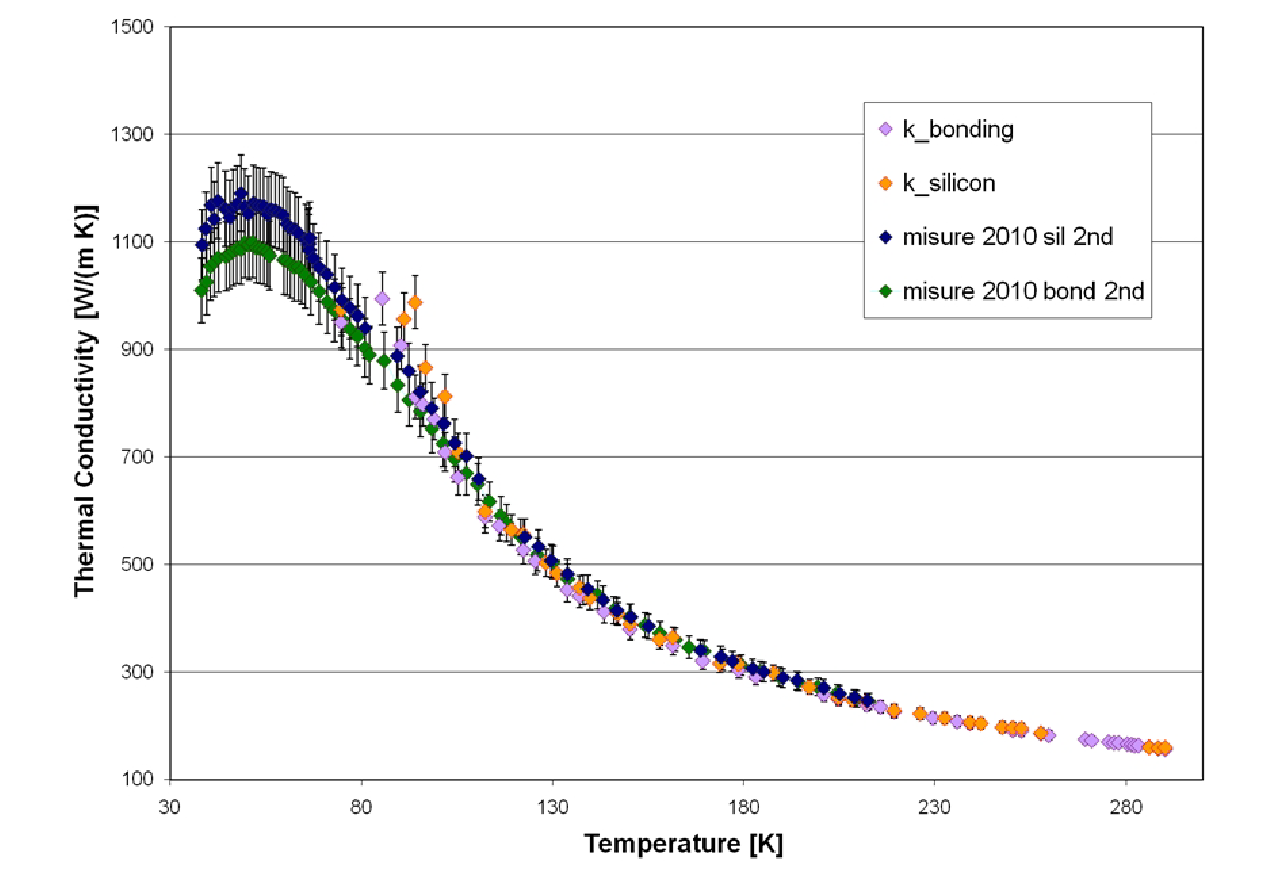
\includegraphics[width=100mm]{Sec_Suspensions/Figures/silicon-bond-thermal-conductivity.pdf}
			\caption{Measured thermal conductivity through silicon rods (1'' diameter, 28 and 48 mm lengths) carried out in Florence.  Bonded samples fabricated in Glasgow.}
\label{fig:silicon-bond-thermal-conductivity}
	\end{center}
\end{figure}

\FloatBarrier
\subsubsection{R\&D on surface losses in silicon}
\label{sec:si_surface_loss}

At cryogenic temperatures the performance of the fibres or  ribbons used as suspension elements will be limited by surface loss (see Fig.\,\ref{fig:susp_loss}). Thus, the study of  the surface loss mechanism is of great interest to minimise the suspension thermal noise.
The wide field of micro-mechanical systems investigated surfaces losses in silicon (see e.g. \cite{Yang2000,Yasumura2000,Yang2002}). However, a systematic and general modelling of surface losses has not been made. The origin of surface losses is still unclear and needs to be investigated.

\begin{figure}[htbp]
\begin{center}
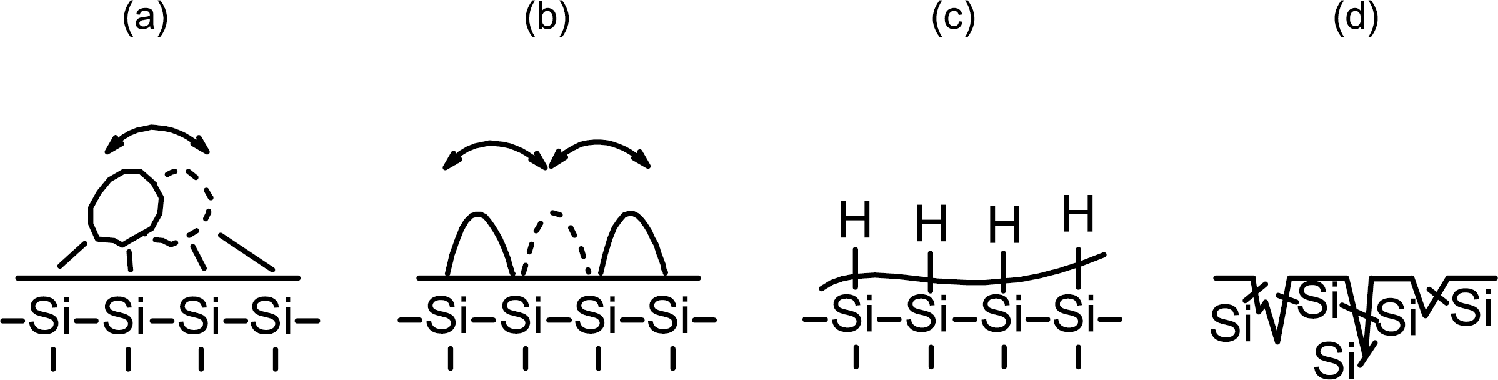
\includegraphics[width=0.75\linewidth]{Sec_Suspensions/Figures/surface_loss.pdf}
\caption{Possible sources of surface losses in silicon (explanation see text).}
\label{fig:surf_loss}
\end{center}
\end{figure}

So far, possible sources of surface losses in silicon have been identified to be (see Fig.\,\ref{fig:surf_loss}):

\begin{itemize}
\item (a) particles on the surface,
\item (b) un-terminated (dangling) bonds,
\item (c) surface layers,
\item (d) micro-cracks in the surface layer due to mechanical treatments.
\end{itemize}

Different treatments of the surfaces lead to different levels of mechanical losses at low temperatures (see Fig.\,\ref{fig:flexure_loss}). A possible correlation with the residual micro-roughness and/or the treatment method is currently under investigation \cite{Nawrodt_2010_arXiv}. Different treatment techniques like wet chemical etching or dry-etching (ion etching) is under investigation and the surface loss parameters are extracted.

For the ET design study a very conservative value of the surface loss has been used. However, any further improvement of surface losses will lead to a lower suspension thermal noise and thus will improve the performance of the detector.



\FloatBarrier
\subsubsection{R\&D on a new generation of monolithic accelerometer for the suspension control.}
\label{sec:accelerometers}
%\emph{
%Author(s): F.\ Acernese, F.\ Barone}

The development of inertial sensors, with high sensitivity and large measurement band is a key point for the inertial damping to perform on the suspension system of third generation interferometric detectors.

In particular we developed a low noise high resolution horizontal monolithic folded pendulum (FP) sensor~\cite{BLAIR-1,FIDECARO-1}. The design is based on the use of micro-machining techniques (to reduce the sensor size to dimensions suitable for placing it in sea floors or in boreholes) and the application of laser optics techniques for the implementation of the sensor readout system (to improve the sensitivity and the  immunity to environmental noises)~\cite{SMART10-1,RSI-1}.

\medskip

%\subsubsection{Mechanical Model}

An accurate description of the dynamics of a Folded Pendulum (FP)  is given by the simplified Lagrangian model developed by J.Liu et al.~\cite{BLAIR-1}, based on the mechanical scheme shown in Figure~\ref{fig:FP_Scheme}. The FP model consists of two  vertical beams of lengths $l_1$ and $l_2$ and masses $m_{a_1}$ and $m_{a_2}$, respectively. The central mass is modelled with two equivalent masses, $m_{p_1}$ and $m_{p_2}$, located near the hinge points at distances $l_{p_1}$ and $l_{p_2}$ with respect to the pivot points of the pendulum arm and of the hinging point of the oscillating mass.
\begin{figure}[h!t]
	\centering
  	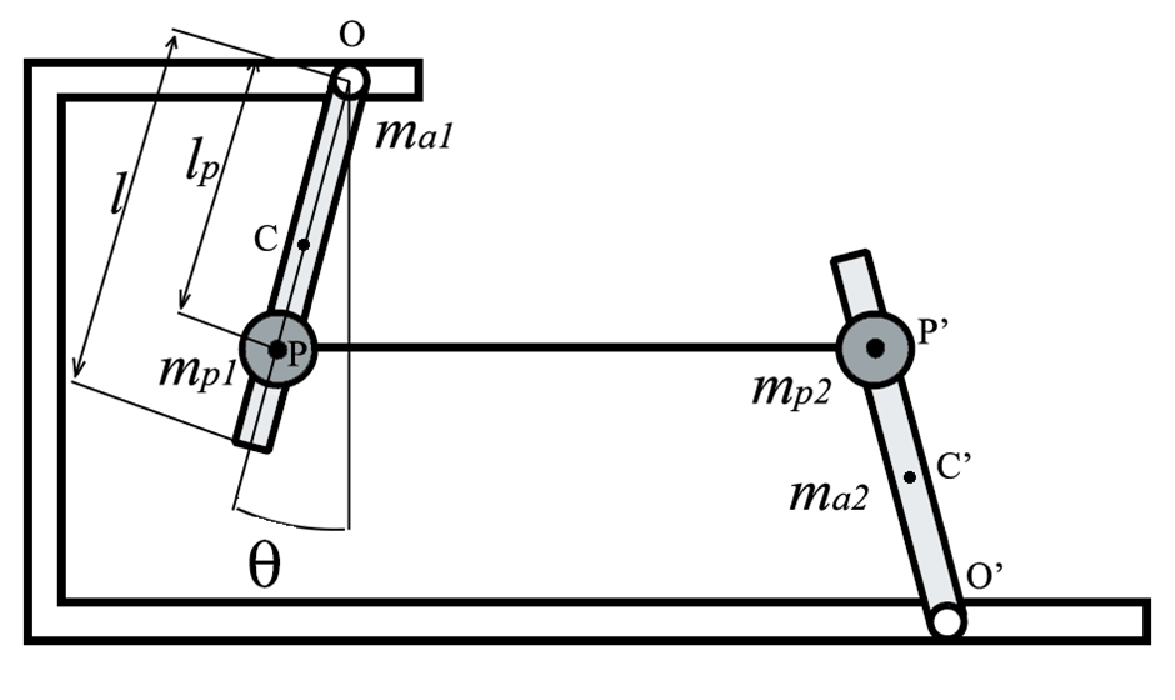
\includegraphics[width=8.5cm]{Sec_Suspensions/Figures/FP_Scheme.pdf}
	\caption{\label{fig:FP_Scheme}Folded Pendulum Mechanical Model}
\end{figure}

Assuming that the centre of mass of the pendula is in $l_{i}/2$ and using the approximation of small deflection angles, then the FP Transfer Function can be easily obtained by solving the Lagrange Equations. Defining the coordinate of the pendulum frame (fixed to the ground) as $x_s$ and the coordinate of the FP central mass as $x_p$ (see Figure~\ref{fig:FP_Scheme}), then the FP transfer function is
\begin{equation}
\label{eq:FP_Transfer_Function}
\frac{x_p(\omega)}{x_s(\omega)} = \frac{\omega_0^2 -A_c \omega^2}{\omega_0^2 - \omega^2} = 1 + \frac{(1-A_c)\omega^2}{\omega_0^2 - \omega^2}
\end{equation}
\noindent
where 
\begin{equation}
\label{eq:FP_Resonant_Frequency}
\omega_0^2 =  \left( \frac{g}{l_p} \right) \cdot \frac{(m_{a_1} - m_{a_2})\frac{l}{2 l_p} + (m_{p_1} - m_{p_2})+ \frac{k}{g l_p}} {(m_{a_1} + m_{a_2})\frac{l^2}{3 l_p^2} + (m_{p_1} + m_{p_2})} 
\end{equation}
is the square of FP resonant angular frequency and 
\begin{equation}
\label{eq:Centre_of_Percussion}
A_c = \frac{\left(\frac{l}{3 l_p} - \frac{1}{2} \right) (m_{a_1} - m_{a_2}) }{(m_{a_1} + m_{a_2}) \frac{l^2}{3 l_p^2} + (m_{p_1} + m_{p_2})}
\end{equation}
is the parameter related to the center of percussion effects~\cite{BLAIR-1}. 

The tuning can be obtained changing the values of the masses $m_{p_1}$ and $m_{p_2}$, adding a tuning mass, $M_l$, at a distance $D$ from the pendulum suspension point.

A better physical interpretation of the dependence of the FP resonant frequency from its physical and geometrical parameters, can be obtained if Equation~\ref{eq:FP_Resonant_Frequency} is rewritten as
\begin{equation}
\omega_0^2 = \frac{(m_{a_1}-m_{a_2})\frac{g l}{2l^2_p} + (m_{p_1}-m_{p_2})\frac{g}{l_p} + \frac{k}{l_p^2}}
{(m_{a_1}+m_{a_2})\frac{l^2}{3 l_p^2} + (m_{p_1}+m_{p_2})} 
\end{equation}
\noindent
Defining the equivalent gravitational constant, $K_{g}$, as
\begin{equation}
K_{g} = (m_{a_1}-m_{a_2})\frac{g l}{2 l^2_p} + (m_{p_1}-m_{p_2})\frac{g}{l_p}
\end{equation}
\noindent
the equivalent elastic constant, $K_{e}$, as
\begin{equation}
K_{e} = \frac{k}{l_p^2}
\end{equation}
\noindent
and the equivalent mass, $M_e$, as
\begin{equation}
M_e = (m_{a_1}+m_{a_2})\frac{l^2}{3 l_p^2} + (m_{p_1}+m_{p_2}) 
\end{equation}
\noindent
then the FP resonant frequency, $f_{o} = \frac{\omega_{o}}{2 \pi}$, can be rewritten as
\begin{equation}
\label{eq:newf0FP}
f_0 = \frac{1}{2 \pi} \sqrt{\frac{K_{g}+K_{e}}{M_e}}
\end{equation}
It is easy to recognize in Equation~\ref{eq:newf0FP} the classic expression of the resonant frequency of a spring-mass oscillator with an equivalent elastic constant $ K = K_{g} + K_{e} $.

\medskip

%\subsubsection{Measurements on the prototype}

The FP mechanical prototype is a monolithic system, shaped with precision machining and electric discharge machining (EDM)~\cite{RSI-1, SMART10-1}. In fact, the monolithic mechanical design has the great advantage of avoiding the shear effects at the contact surface among mechanical parts that can generate hysteresis and dissipation in a non monolithic structure~\cite{BLAIR-1}. The result is a very compact sensor, with a high Q-factor (the Q factor of the material) and a good thermal sensitivity that guarantees a very good sensor directivity: coupling factors of less than $10^{-4}$ among the different degrees of freedom have been obtained in monolithic structures~\cite{FIDECARO-1}.

The four torsional flexures, connecting the pendulum arms to the central mass and to the frame, have an elliptical profile with $100\,\mu m$ minimum thickness with ellipticity ratio of $\epsilon = 16/5$. The pendula arms are designed to minimise the mass and the moment of inertia without reducing rigidity and symmetry. The values of the masses of the pendulum arm, of the inverted pendulum arm and of the central mass are $m_{a_1} \approx 40\,g$, $m_{a_2} \approx 50\,g$ and $(m_{p_1}+m_{p_2}) \approx 600\,g$, respectively. 

The tunability of the monolithic FP natural frequency was obtained machining several drilled holes for fixing suitable shaped and positioned tuning masses, as predicted by Equation~\ref{eq:FP_Resonant_Frequency}. In fact, tuning the FP at its lowest possible natural frequency maximises the sensor measurement band at low frequencies. But, the lower is the natural resonance frequency, the lower is the restoring force of the pendulum to external perturbations. Furthermore, a lower natural resonant frequency permits to relax the specifications of the control system for force feedback sensor configuration. The drawback of soft restoring forces is that the test mass easily touches the frame, saturating the sensor. Therefore, the gaps between the central mass-arms and arms-frame was set at  2\,mm. In this way the dynamics of the monolithic FP sensor is  quite large, but still far from the elastic limit of the material. These large gaps have another vantage when the FP works in air. In fact, the $Q$ of the instrument in air is strongly influenced by the damping effect of the air present in these gaps, that largely reduces its value. This effect reduced the value of $Q$ from $Q = 3000$ in vacuum to values of $Q=3$ in air~\cite{FIDECARO-1}. Our technical choice allowed us to obtaining a measured value of $Q = 140$ in air, perfectly acceptable for an use of monolithic FP as sensor.

The measurement of the transfer function was made using a standard measurement procedure used in control theory to obtain the transfer function of a linear system using white noise. For this task the central mass, $m_{p}$, was excited with white noise (input signal) through the coil-magnet actuator while the output signal, that quantifies the central mass motion, was read with the optical lever readout. Then the transfer function of the monolithic FP is obtained by simply dividing the output spectrum by the input one. The results of this first test are shown in Figure~\ref{fig:TF}, where both the theoretical model and the experimental points are reported. We notice the very good agreement between  the data and the predictions, which supports our confidence in the  theoretical model. The analysis of these data show the natural \emph{design} resonance frequency of the monolithic FP is $720 \pm 5$\,mHz with a $Q \approx 140$ in air.

\begin{figure}[h!tb]
	\centering
		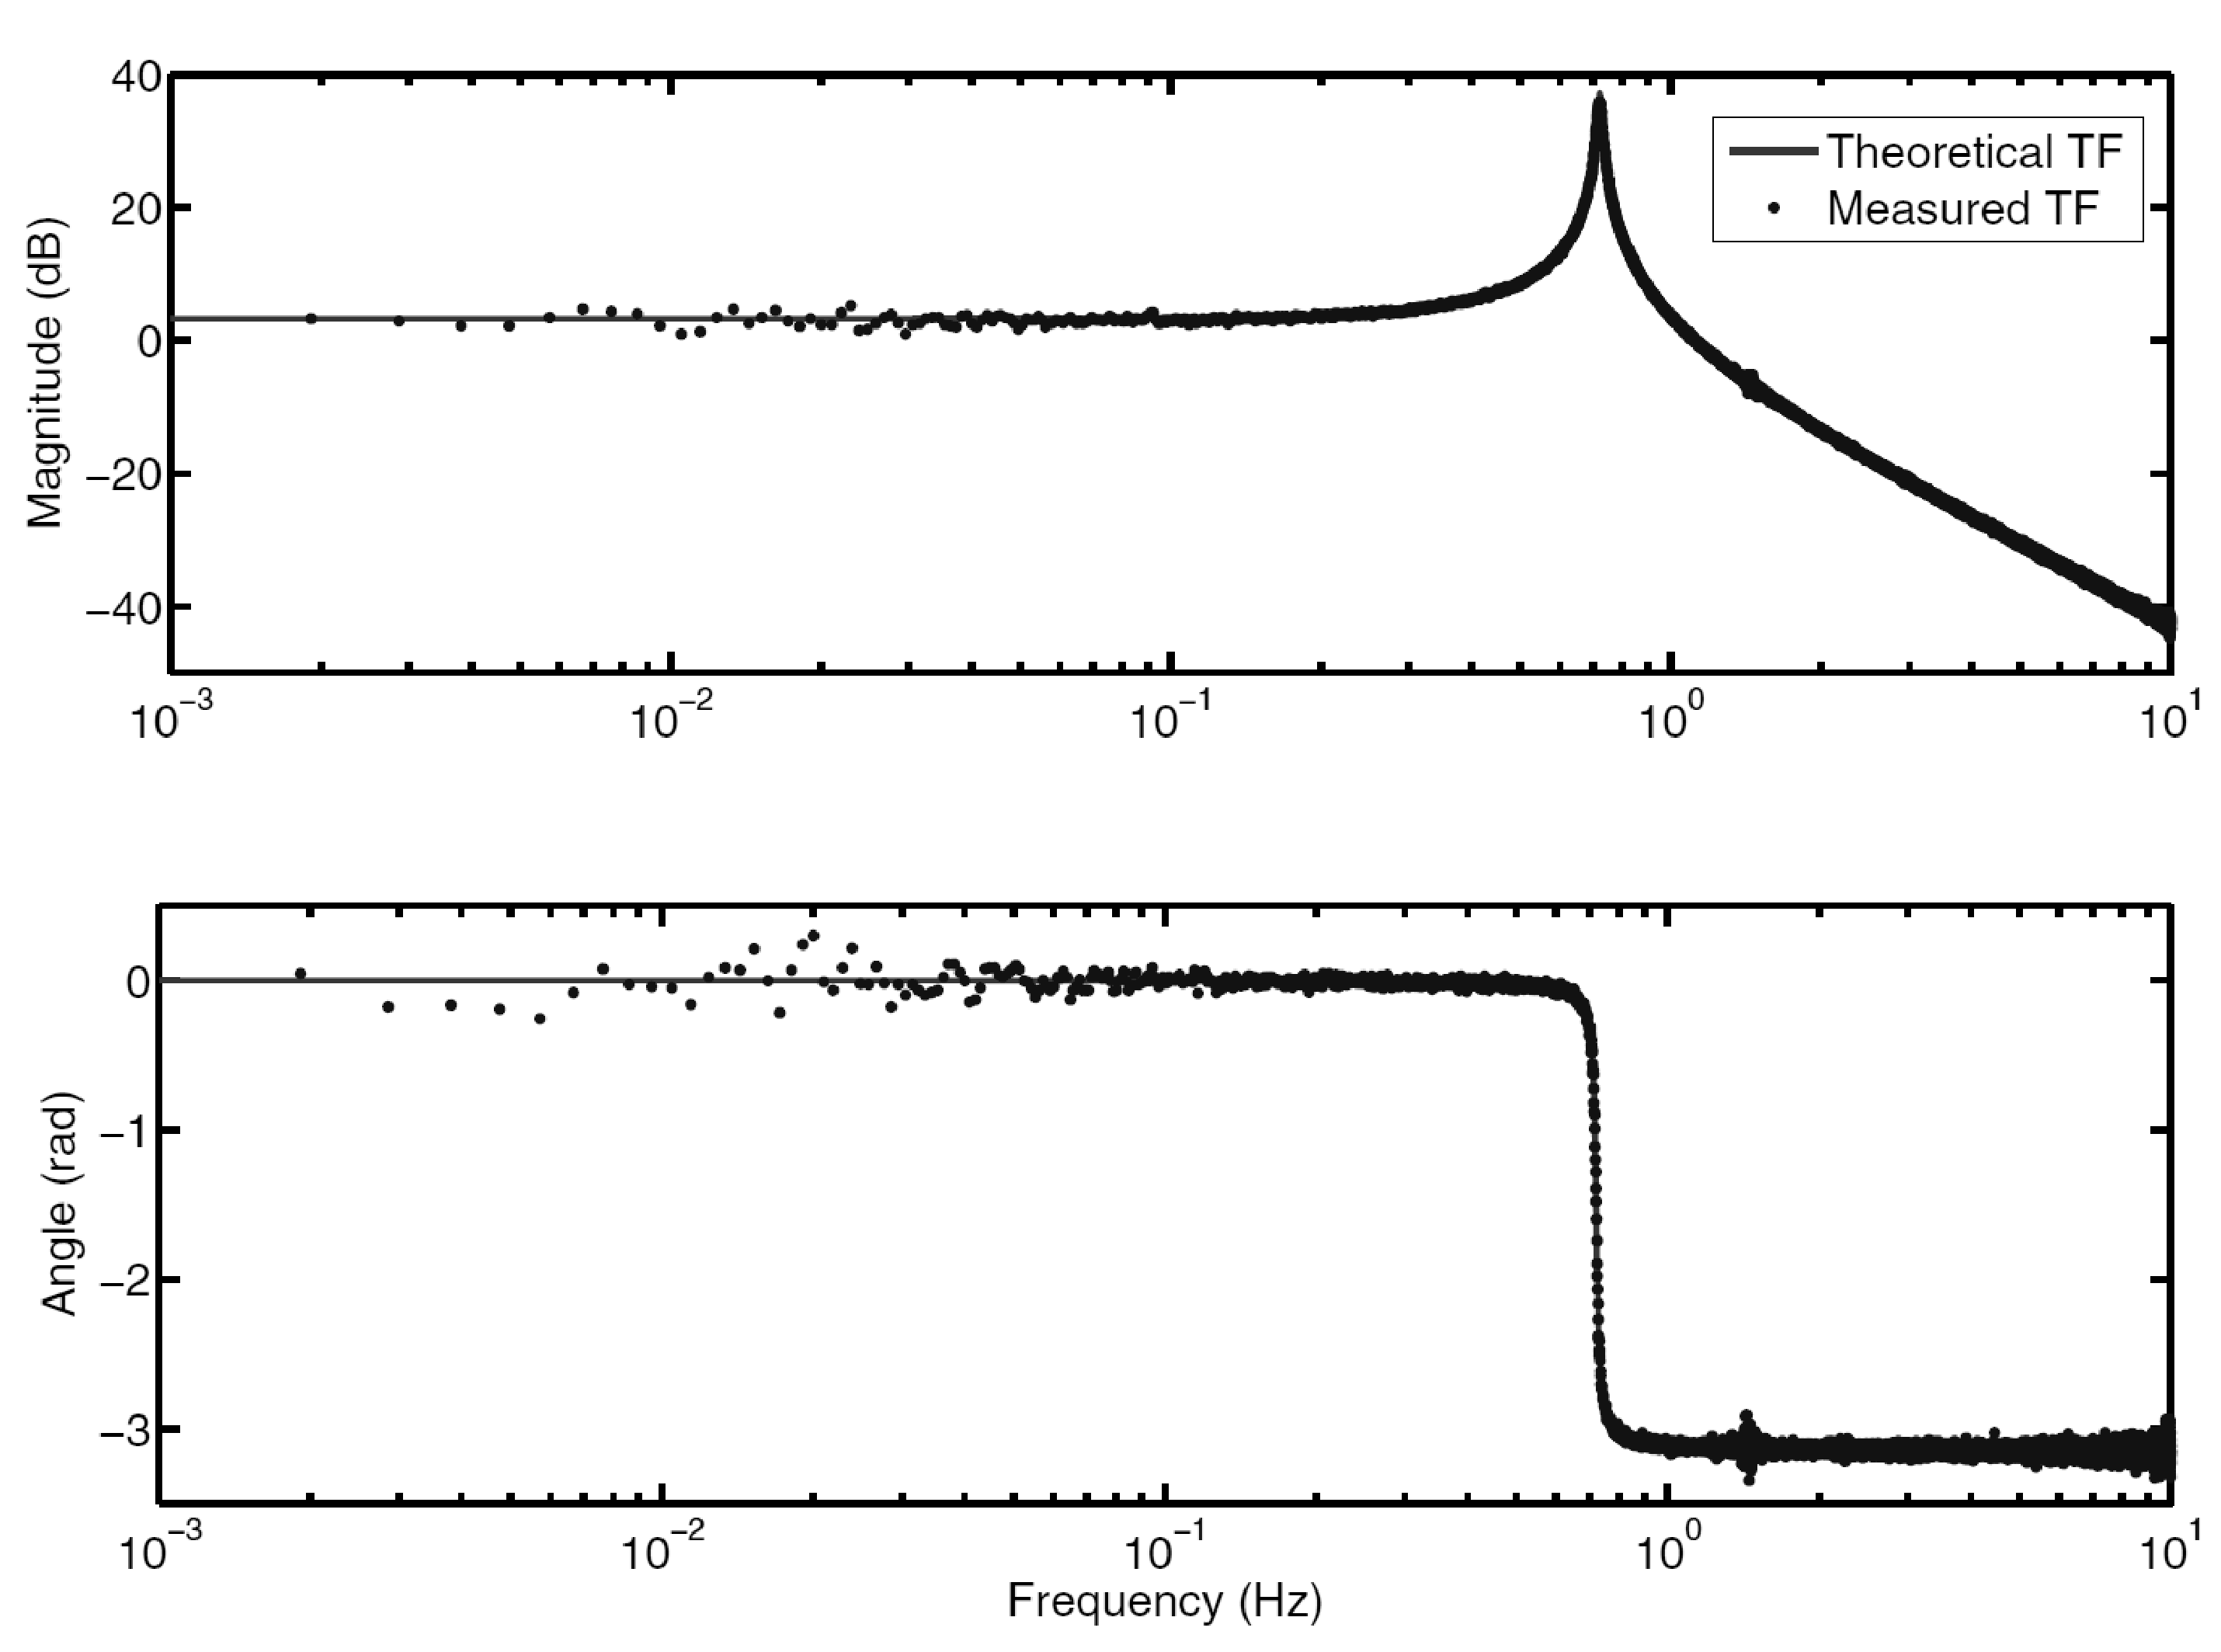
\includegraphics[width=8.5 cm]{Sec_Suspensions/Figures/FP_TF.pdf}		
   	\caption{Theoretical and experimental Transfer Function of the horizontal monolithic FP.}
	  \label{fig:TF}
\end{figure}

To test the tuning procedure, we used tuning masses of different weights, in order to implement a rough or fine calibration, positioned in the opening of the test mass. The FP sensor was positioned on a platform for levelling. The tuning masses were moved in small steps, of less than 1\,mm. 
\begin{figure}[!htb]
  \centering
	   \includegraphics[width=8.5 cm]{Sec_Suspensions/Figures/FP_Frequency.pdf}
	   \caption{\label{fig:FP_Experimental_Frequency_Tuning} Measured resonance frequencies of the horizontal monolithic Folded Pendulum sensor. The best measured frequency, $f_{r} = 70$\,mHz, is circled.}
\end{figure}

We made different sets of measurement to evaluate the stability of the measurement procedure. In Figure~\ref{fig:FP_Experimental_Frequency_Tuning} the measured frequency versus the tuning mass position is shown. The data were interpolated using Equation~\ref{eq:FP_Resonant_Frequency} with adaptive parameters $(m_{p_1}+m_{p_2})$ and $k$. Figure~\ref{fig:FP_Experimental_Frequency_Tuning} shows the very good agreement between the experimental data and the $3 \sigma$ error bars of the theoretical model. The three sets of measurements performed over 10 days fall on the same curve within errors. The interpolation parameters with an error bar with a level of significance $\alpha=0.05$ are in good agreement with the experimental ones, such as the distributed masses and the angular stiffness interpolated are in good agreement with the measured ones in this case, too.

The second step was a direct measurement of the $Q$ of the monolithic FP sensor. For this task we performed a set of measurements in air in order to obtain an experimental curve expressing $Q$ as function of the monolithic FP resonance frequency, $f_{o}$. We are well aware that these measurements are largely dependent also on the environmental conditions, but they are important to obtain an empirical physical law for our prototype, useful to predict the values of $Q$ at different resonance frequencies. For this task we used a tuning mass of $M_{l} = 120 \, g$.
The results of this set of measurement are reported in Figure~\ref{fig:Q}, where it appears evident that all the measurements follow a linear law. In fact fitting the data we obtained a confidence factor equal to $R=0,95$.

\begin{figure}[h!tb]
	\centering
		\includegraphics[width=8.5 cm]{Sec_Suspensions/Figures/Q2.pdf}		
   	\caption{Mechanical quality factor versus resonant frequency for FP sensor in air.}
	  \label{fig:Q}
\end{figure}




\FloatBarrier
\subsection{The cost evaluation of the suspension system}
\label{sec:suspension_cost}
%\emph{
%Author(s): F.\ Frasconi, E.\ Majorana, M.\ Lorenzini, R.\ Nawrodt , P.\ Puppo, S.\ Reid, F.\ Ricci}

The cost of the various items are reported in the final chapter of this book. Here we summarize just the guidelines for its evaluation.
The suspensions system has a relevant impact on infrastructure: it constraints the cavern dimensions and  requires auxiliary installation on site for the assembly. Items listed below  have to be  included in the infrastructure budget.

\begin{itemize}
\item {Clean rooms for payload assembly}
\item{Payload washing machine}
\item{Facility for the construction of the silica fibres}
\item {Facility for the construction of the silicon fibres}
\item {Low vibration electric vehicle for payload transport}
\item{ Vacuum oven for thermal treatments}
\end{itemize}

 The evaluation of the suspension cost for the ET-HF interferometer  is based on the Virgo investment updated for the Euro currency  inflation. It concerns:

\begin{itemize}

\item {Superattenuator filters}
\item{Inverted pendulum}
\item{Cables and wires}
\item{Suspension electronics}
\item{Safety structure}
\item {Payload mechanics}
\item {Assembly tools}
\item{Sensors and actuators}
\item{Local system control}
\end{itemize}

The ET-LF case includes extra cost to the respect of the ET-HF case. In particular we have to consider
  

\begin{itemize}
\item{ The mechanics for  the interface separating the upper and lower suspension system}
\item {The reviewed cost estimation for the longer Superattenuator}
\item { The Superattenuators hosted in the ancillary towers}
\item {The active vibration dumping included in the cryogenic solution based on the pulse tube }
\item {The reviewed cost estimation for the cryogenic payload}
\item{Temperature monitor and control}
\item{ The reviewed cost of the local system control for the mirror at low temperature}
\end{itemize}

For the cryogenic payload cost we based the evaluation on the experience gained on  the system  set up for the R \& D FP6 - ILIAS- STREGA  project \cite{cryo_payload}.
